\documentclass[a4paper,11pt,oneside,openany]{book}
\usepackage[left=1.5in, right=1in, top=1in, bottom=1in, includefoot, headheight=13.6pt]{geometry}
%\documentclass{octavo}
%\usepackage[DIV=9,a4paper,pagesize]{typearea}
\usepackage{fancyhdr}
\usepackage[toc,page]{appendix}
\usepackage{amsfonts,amssymb,amsmath,mathrsfs,nccmath}
\usepackage{float,graphicx}
\usepackage{todonotes}
\usepackage[bottom]{footmisc}
\usepackage{pdfpages}
%\usepackage{media9}
\usepackage[breaklinks=true]{hyperref}
\usepackage{verbatim}
\usepackage{pgf}
\usepackage{verbatimbox}
\usepackage{xcolor}
\usepackage{import}
\usepackage{cleveref}
\usepackage{makecell}
\usepackage[normalem]{ulem}
\usepackage{tabu}
\usepackage{gensymb}
\usepackage{tikz}

\usepackage{tzplot}
\usepackage[makeroom]{cancel}
\usepackage{multirow}
\usetikzlibrary{math} %needed tikz library
\usetikzlibrary{shadings,shapes,arrows,patterns,calc,intersections}
\usetikzlibrary{arrows.meta}
\usepackage{subfig}
%\usepackage[inkscape={C:/Program Files/Inkscape/bin/inkscape}]{svg}

%%%%% bibliography
\usepackage[round,sectionbib]{natbib}
\usepackage{chapterbib}    
%\usepackage{filecontents}
\usepackage{empheq}
\usepackage[many]{tcolorbox}
\usepackage{booktabs}% http://ctan.org/pkg/booktabs
%%%%%%%%%%% commands
\newcommand{\ag}[1]{\textcolor{blue}{#1}} 
\newcommand{\mb}[1]{\textcolor{green}{#1}}
\newcommand{\dlv}[1]{\textcolor{red}{#1}}
\newcommand{\ud}{\mathrm{d}}
\newcommand{\de}[2]{\frac{\ud #1}{\ud #2}}
\newcommand{\diag}{\mathrm{diag}}
\newcommand{\bra}[1]{\langle #1|}
\newcommand{\ket}[1]{|#1\rangle}
\newcommand{\braket}[2]{\langle#1|#2\rangle}
\DeclareMathOperator{\Tr}{Tr}
\newcommand{\sech}{\mathrm{sech}}
\newcommand{\sgn}[1]{\mathrm{sgn} #1}
\newcommand{\pdern}[3]{\frac{\partial^#3#1}{\partial#2^#3}}
\newcommand{\pder}[2]{\frac{\partial#1}{\partial#2}}
\newcommand{\Res}{\operatorname{Re}}
\let\Eps\varepsilon
\newcommand{\la}{\lambda}
\newcommand{\lag}{\mathrm{Lag}}
%%%%% colors for the metrics chapters from  Paul Tor's site.
\definecolor{col1}{RGB}{221,170,51}
\definecolor{col2}{RGB}{187,85,102}
\definecolor{col3}{RGB}{0,68,136}
\definecolor{matlaborange}{HTML}{D95319}
%%%%opening 
\title{EWS report}
%\author{ Gomel, Alexis }

\begin{document}
	
	%\include{Chapters/cover1}
	
	\newpage
	\pagenumbering{roman}
	%	\include{titlepage}
	
	%	\include{certificate}
	%	
	%	\include{dedication}
	
	%	
	%	\frontmatter
	%		
	%	\maketitle
	%	
	\maketitle
	\newpage
	\clearpage

	%	
	\newpage
	
	\tableofcontents{}
	%	\mainmatter
	\clearpage
	\pagenumbering{arabic}  % start arabic page numbering
	\setcounter{page}{1}
	
	\pagestyle{headings}
	
	\newpage
		\newpage
	\pagestyle{fancy}
	\fancyhead{}
	\fancyhf{}
	\fancyhf[HR]{\thepage}
	\renewcommand{\chaptermark}[1]{%
		\markboth{\thechapter.\ #1}{}}
	\fancyhead[L]{\textsl{\leftmark}}
	


\chapter{Introduction}

%\fancyhf[EHC]{Introduction}


%\fancyhead[CE]{Introduction}

One of the big challenges of studying and modeling dynamical systems is their nonlinear behavior. 
As an example on how nonlinearities might arise, we can look at a simple pendulum like the one in \cref{fig:pendulum} where a mass is linked to a fixed pivot point, by a mass-less inextensible wire.
It is a first year physics exercise  to show that, for a small perturbation, this pendulum will oscillate around its equilibrium point with a constant amplitude, since the motion depends on the length of the wire and the gravitational constant. 
\begin{figure}[htb]
	\centering
	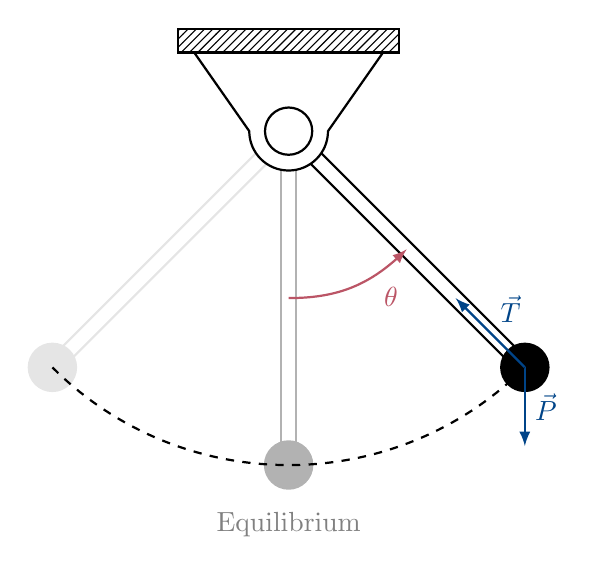
\begin{tikzpicture}[thick,>=latex]
		
		\begin{scope}
			\coordinate (l) at (-3,-3);
			\coordinate (m) at (0,-4.24);
			\coordinate (r) at (3,-3);
			\coordinate (o) at (0,0);
			% left
			\draw[double distance=1.6mm,color=black!10] (o) -- (l);
			\draw[draw=black!10,fill=black!10]  (l) circle (.3cm) node [] (cl) {};
%			(l) node[circle,fill=red!20] (cl) {third node}
			%	\draw let \p1=(l) in (\x1,-5) node {left};

			% middle
			\draw[double distance=1.6mm,color=black!30] (o) -- (m);
			\draw [draw=black!30,fill=black!30] (m)  circle (.3cm);
		%	\node[draw=black!30,circle,fill=black!30,inner sep=0.3] (cm) at (m) {};
%			    \draw (p2) circle (\radius) node [] {};
			\draw[draw=black!30] let \p1=(m) in (\x1,-5) node {\textcolor{gray}{Equilibrium}};
			
			% right
			\draw[double distance=1.6mm] (o) -- (r);
			\draw[draw=black,fill=black] (r) circle (.3cm) node [] (cr) {};
			%	\draw let \p1=(r) in (\x1,-5) node {right};
			\draw[-latex,color=col3] (r) -- node[right]{\textcolor{col3}{$\vec{P}$}}++(0,-1);
			\draw[-latex,color=col3] (r) -- node[above right]{\textcolor{col3}{$\vec{T}$}}(-45:3);
			
%			\draw[dashed,->] (cl.east) to [bend right=45] (cr.west);
%			\draw[dashed,->,left color=black!10, right color=black,shading angle=90,anchor=east] (l.east) to [bend right=45] (r.west);	
			\draw[dashed,->,anchor=east] (l) to [bend right=45] (r);
			\coordinate (lest) at ($(m.east)!0.5!(o.east)$);
			\draw[->,color=col2] (lest) to [bend right=22.5] ($(r.west)!0.5!(o.west)$);
			\node at (1.3,-2.1) {\textcolor{col2}{$\theta$}};   
			
			\draw[fill=white] (-1.2,1.0) -- (-.5,0) arc(180:360:0.5) -- (1.2,1.0) -- cycle;
			\draw[draw=black,fill=white] (o) circle (.3cm);
			\draw[pattern=north east lines] (-1.4,1.3) rectangle (1.4,1);
			
		\end{scope}
		
	\end{tikzpicture}
	\caption{Scheme of a simple pendulum where a mass oscillates around a stable equilibrium due to its own weight \textcolor{col3}{$\vec{P}$}, and a constraint force given by the tension \textcolor{col3}{$\vec{T}$}. The angle \textcolor{col2}{$\theta(t)$} measure the displacement from the equilibrium.}
	\label{fig:pendulum}
\end{figure}

This simple result allowed Christian Huygens in 1656 to make the first pendulum clock, being able to measure time  accumulating an error of something less than a minute per day. 
However, this periodicity stems from an approximation and if the oscillations are large enough, or we want to estimate the error we are accumulating, we would have to consider a more complex approximation or the full nonlinear expression of the restoring force. 


If we want to go further and  describe the oscillation in a as precise as possible manner,  we  need to  consider that the wire is not an ideal object and will stretch and contract due to the changes in the tension of the pendulum, a model which can display chaotic behavior \citep{Cencini2009}. 
Moreover, the system can be complicated by including the effect of friction on the pivot point, the air resistance, or the fact that, being at a given temperature, there are radiative losses due to its black body radiation.
%If we want to know how long and this system can continue oscillating losses due to friction in the pivot point, and if we take it to the extreme we could describe the whole system at a given temperature and therefore will have losses due to its black body radiation.

In general, the degree of complexity of our model will depend on the question we want to answer. Are we interested in making a time measuring device which is accurate at the scale of minutes and only needs maintenance at the scale of months or years?  Do we need a time keeping device that can work for decades? Do we need to resolve time scales smaller than a second? Can we put our device in any environment? What happens if we include some external forcing?


% when there is no stable equilibrium but the systems stays bounded in phase space by a strange attractor,
	
%\begin{figure}
%	\centering
%	\includegraphics[width=0.5\linewidth]{Images/Introduction/backbone_curve.png}
%	\caption{Resonance or backbone curve or a nonlinear system as shown in \citep{Londono2015}. }
%	\label{fig:backbone}
%\end{figure}



Lots of problems are nonlinear because the level of description we want in our model requires them to be so.
In general, the systems of interest in the real-world can be complex and be comprised of several interacting pieces making their study too hard to be understood from first principles (biological systems, complex networks, models of disease spread), inapplicable (finance, network dynamics), or not needed (social dynamics). 
In these cases, nonlinear models are developed to capture the dynamics of such systems to some degree of accuracy. 


%\begin{tikzpicture}[font=\footnotesize]
%	
%	% Support
%	\fill (-1.5,0) rectangle(1.5,0.1);
%	
%	% Bob's trajectory
%	\draw[dashed] (-60:4) arc(-60:-120:4);
%	
%	% Rod + Bob
%	\draw (0,0) -- (-60:4) node[fill,circle](m){};
%	
%	% Weight Force
%	\draw[-latex] (m) -- node[right]{$\vec{P}$}++(0,-1) ;
%	
%	% Tension Force
%	\draw [-latex] (m) -- node[right]{$\vec{T}$}(-60:3);
%	
%	% Light gray pendulum
%	\draw[black!10] (0,0) -- (-90:4) node[fill,circle]{};
%	\draw[black!10] (0,0) -- (-120:4) node[fill,circle]{};
%	
%\end{tikzpicture}


Known nonlinear models like the physics of birdsong \citep{Mindlin2005}, or models for population dynamics, chemical reactions, light propagation, can recover global behavior like epidemics \citep{Southall2021}, population extinctions \citep{Jackson2001}, nonlinear oscillations \citep{Diz-Pita2021}, light self-focusing \citep{Bejot2011}, etc.. 

While systems near equilibrium  or steady state can usually be approximated by linear equations, this approach is no longer applicable when far from the equilibrium, for example under the action of a large forcing \citep{Londono2015}.% amplitudes, or they might no even be linearizable in the first place, like chaotic systems. 
Other systems are  intrinsically nonlinear, like the fluid motion described by the Navier-Stokes equation or the gravitational field described by the Einstein theory of general relativity.% even when deduced by first principles, most notably the Navier-stokes which describe the behavior of fluids, and  the Einstein field equations in general relativity.


These non-linear systems are seldom solvable in an analytical form, and exhibit several behaviors not present in linear systems. Even simple one-dimensional continuous systems can display bifurcations, hysteresis, multi-stability, and in three or more dimensions can display chaos like the non-autonomous pendulum, with high sensitivity to initial conditions,  arbitrary close trajectories becoming exponentially different as time evolves. 


Stanislaw Ulam, a Polish-American mathematician and physicist who participated to the Manhattan Project, reportedly once remarked:- "Using a term like nonlinear science is like referring to the bulk of zoology as the study of non-elephant animals.” -.
This is to say, nature, more often than not,  is nonlinear.
Given this \textbf{zoo} of behaviors it is clear that a key problem when studying nonlinear systems is the capacity to predict their behavior, in particular when they  display big fluctuations, but also when they can suddenly change their state. 

There are mathematical tools, such as normal forms, that allow one to infer similarities between different nonlinear systems and understand some of their universal properties\footnote{Normal forms \citep{Strogatz2000} are a tool to rewrite the nonlinear models in terms of new variables that are more 'natural' for the dynamics. In general, if one can prove that two models of different systems have the same normal form within a range of parameters, then  there is a mathematical path to understand one system in terms of the other.}. 
Of particular importance for this thesis is the nonlinear Schrödinger equation (NLS), which appears  in a wide variety of nonlinear systems and allows researchers in different areas to be inspired by results in other fields, as well shown in works where analogies between light intensity in fiber optics and the envelopes of surface gravity waves are made \citep{Solli2007}.

The prediction of rare and large deviations\footnote{Here, large deviations  also include extremely low values with respect to the normal.\ag{correct by maura 8/1. NOrmal refers to the expected distribution, not just the mean.}} from the normal events, or extreme events, is of particular interest for areas like finance where market crashes are big disruptive events with huge consequences on social systems. 
But such events can be found  as well in natural systems, like in earth tectonics, ocean waves, and other processes that involve interacting structures at different scales, transitions towards critical points \citep{Sornette2002}, sudden chaotic explorations \citep{Gomel2019}, or nonlinear self amplification \citep{Onorato2021}.
Following a definition originally coined in finance, rare events are sometimes classified as 'black swans' when they are statistically expected given a normal\footnote{In the sense of being explained by only one stochastic mechanism that results in a power law tail distribution, and are scale-invariant and self-similar.} behavior of the system and cannot be predicted, and 'dragon kings' when the extreme events need a particular deterministic mechanism to occur and thus might be predicted \citep{Sornette2009a}.

For surface gravity waves, extreme events or "rogue waves'' can occur both through random linear superposition \citep{Fedele2016},  in this case being analogous to 'black swans'.
However some rogue waves need nonlinear mechanisms to be explained \citep{Onorato2021,2013PhR...528...47O}, where the wave modes can exchange energy between each other, in this case being analogous to 'dragon kings'. %\ag{I don't feel 100\% sure about this analogy, if some of you know Sornette's papers i'd like to have a second opinion. Here is a lighter read \url{https://en.wikipedia.org/wiki/Dragon_king_theory}. I might be cornering myself into something that is not valid just for the sake of making a fun analogy.}
%\color{red}
Prediction of a sudden, big, change in behavior due to a small change is a problem of interest in many fields, from engineering, ecology, climate science, psychology, physics, finance, economics, medicine, etc..  
%
This Critical transitions have received different names in different fields, in physics this are usually called 'phase transition', in climate science this are called 'tipping points', while in ecology are referred as 'regime shifts' while in economics have been described as 'economic catastrophes' \citep{Kopp2016, Feudel2018}.
%
The phrase “tipping point” appears to have originated in industry, where it referred literally to the point at which an engineered system, such as a rail wagon of coal in a Yorkshire foundry \cite{burnley1871} or a cup in a tilting water meter \cite{Hoadley1883}, tipped over and emptied its contents. The earliest use of the term in academic research occurred in the social sciences. In a Scientific American article on racial segregation, the political scientist Morton Grodzins applied the phrase “tipping point” to a critical proportion of non-whites in a neighborhood, above which the fraction of whites precipitously declines to zero.
%
in particular this is a high priority problem given the challenges we face due to climate change. Indeed, it has been shown that several ecological and climate systems can change drastically due to either a big perturbation that might move the system to another stable solution or due to a bifurcation by a slow change of some parameter \cite{Clements2018a, Bathiany2016, Lenton2011, McKay2022}. 
%\color{black}

%
%\color{red}
%Finally, in chapter \ref{ch: ews}  we change to explore the possibility of predicting changes in the qualitative behavior of dynamical systems. 
%There we will give a summary on tipping point, a subject which we have started exploring, and show some preliminary explorations and results
%\color{black}

%
%\subsubsection{resources}
%
%The importance of tipping point in our climate and bioms has lead to the creation of several organizations that keep track of historical data and possible tippings in many systems. 
%Such as the fishery crisis website, \url{http://fisherycrisis.com/}, which tracks sea life abundance for several species all over the globe. 
%\url{https://www.thetippingpoints.com/} ... 
	%	\input{Chapters/Extreme_events.tex}
	\clearpage
	
	\newpage
	%
%
%\definecolor{color_s}{rgb}{0.3922, 0.7059,   0.6667} 
%\definecolor{color_Ns}{rgb}{0.9765,  0.4431,   0.4431} 
%\definecolor{color_utr}{rgb}{0.631,0.733,0.333} %blue main frequency
%\definecolor{color_main}{rgb}{0.141,0.118,0.306} %blue main frequency
%\definecolor{color_sideband}{rgb}{0.855,0.675,0}  %yellow 1st sideband
%\definecolor{color_2sideband}{rgb}{0.525,0.20,0.435} %purple 2nd sideband
%\definecolor{newblue}{rgb}{0, 0.4470, 0.7410} %dispersion
%\definecolor{newred}{rgb}{0.6350, 0.0780, 0.1840} %nonlinearity
%\definecolor{scolor}{rgb}{0.18824, 0.45882 0.8759} %start
%\definecolor{ecolor}{rgb}{0.87451, 0.30588, 0.75294} %end



\chapter{Tipping mechanisms, and early warning signals.}
\label{ch: ews}
%
In the previous chapters, we focused on a nonlinear mechanism by which the system can shift from on state to another by changing an external parameter (the bathymetry) in a deterministic manner.


%a system might display extreme evens, in particular how to develop reduced models that allow us to gain insight on how nonlinearity plays a role in the modulation of wave packets in surface gravity waves.

In this chapter, we will focus on another  problem specific to nonlinear systems: the prediction of regime  changes.

Dynamical systems can, not only change their stability or periodicity, but they can also have the property of having several stable states (attractors) which can coexist for a given set of parameters and/or forcings.
This property is referred as multi-stability; which means a system might also change, or flip, state between multi-stable solutions.

The field of early warning signals (EWS) studies the methods to predict systems going through sudden changes in behavior when they change from one state to another.
A system abruptly changes its behavior, due to a small change in some parameter. 

One of the ways in which a system can move from one stable state to another is trough a critical transition. 
\Cref{fig: stability_example} exemplifies this effect with a system where a change of sign of the parameter $\la$ changes abruptly the stable solutions of the system.  Therefore, any small change in the parameter that leads to a change of sign has big implications for the state of the system. 



\begin{figure}[htb]
	\begin{center}
		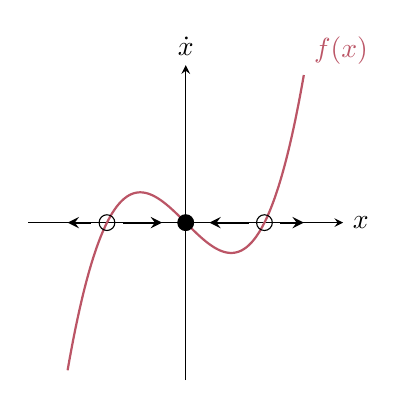
\begin{tikzpicture}
			\tzaxes(-2,-2)(2,2){$x$}{$\dot{x}$}
			\tzfn[col2,thick]{(\x)*(\x-1)*(\x+1)}[-1.5:1.5]{$f(x)$}[ar]
			\draw [->,thick](0.8,0) -- (0.3,0);
			\draw [->,thick](-0.8,0) -- (-0.3,0);
			\draw [->,thick](1.2,0) -- (1.5,0);
			\draw [->,thick](-1.2,0) -- (-1.5,0);
			\node (a) at (0,0) {};
			\filldraw (a.center) circle [radius=0.1cm];
			\draw (a)+(1,0) circle [radius=0.1cm];
			\draw (a)+(-1,0) circle [radius=0.1cm];
		\end{tikzpicture}  \qquad \qquad
		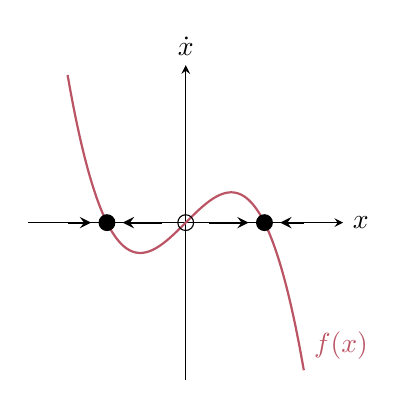
\begin{tikzpicture}
			\tzaxes(-2,-2)(2,2){$x$}{$\dot{x}$}
			\tzfn[col2,thick]{-(\x)*(\x-1)*(\x+1)}[-1.5:1.5]{$f(x)$}[ar]
			\draw [->,thick](0.3,0) -- (0.8,0);
			\draw [->,thick](-0.3,0) -- (-0.8,0) ;
			\draw [->,thick](1.5,0) -- (1.2,0) ;
			\draw [->,thick](-1.5,0) -- (-1.2,0) ;
			\node (a) at (0,0) {};
			%	\node[circle,draw,minimum size=10cm] (a) at (0,0) {};
			\draw (a.center) circle [radius=0.1cm];
			\filldraw (a)+(1,0) circle [radius=0.1cm];
			\filldraw (a)+(-1,0) circle [radius=0.1cm];
			%	\tzfn'[red,thick]{(\x)^2}[-1:2]{$f^{-1}(x)$}\\[ar] % inverse
		\end{tikzpicture}
	\end{center}
	\caption{Stability of $\dot{x}=\lambda (x+1)x(x-1)$. If $\lambda >0$(left) then the only stable solution is $x=0$; for $\la<0$(right) the system has two stable solutions $x={-1,1}$. $\la=0$ marks a critical transition for this system.}
	\label{fig: stability_example}
\end{figure}



Tipping points have been identified or are suspected in many systems, from climate \citep{Cai2016,Lenton2011,Boers2017}, phase transitions \citep{Fullsack2022}, fluid dynamics \citep{Lucarini2014,Yang2021}, to seizures \citep{no_cls_epileptic}, population dynamics \citep{10.1086/681573,Bathiany2016} as exemplified in (\cref{fig: climate_bistability}), social dynamics \citep{SCHEFFER2020a}, disease outbreaks \citep{doi:10.1098/rsbl.2019.0713}, cell-death \citep{Sarkar2019}.



\begin{figure}[bhtp]
	\centering
	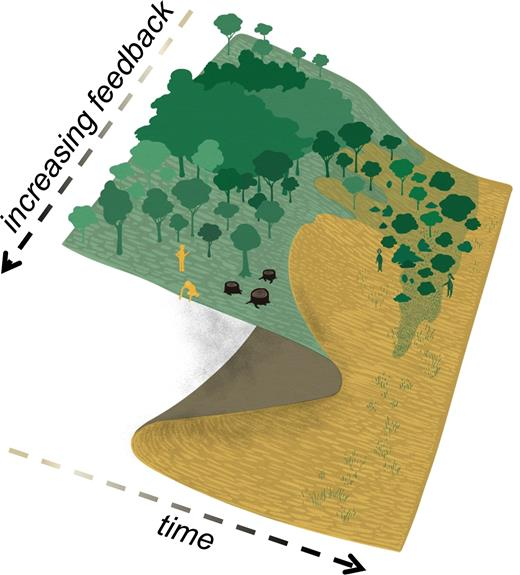
\includegraphics[width=0.4\columnwidth]{Images/Metrics/sahel_multistable}
	\caption{Stability landscape of the Green Sahara and desert. The larger the atmosphere–vegetation feedback (i.e. moving towards the lower left of the figure), the sharper the transition between the two states. (Modified from Model Calendar 2015, designed by Elsa Wikander at Azote, funded by the Beijer Institute of Ecological Economics and the Stockholm Resilience Centre.) Taken from \cite{Bathiany2016}.}
	%	\caption{Events per ms}
	\label{fig: climate_bistability}
\end{figure}



%To provide an early warning to such transitions, dynamical approaches have been proposed, in particular critical-slowing-down  \cite{Scheffer2009,Scheffer344,doi:10.1111/j.1600-0706.2012.20838.x}. However these dynamical approaches impose to observe the system evolution over time after a perturbation. 

%
%%%% this can go somewhere else %%%%           

%Predicting this transitions can be very challenging, in real systems it is often difficult to distinguish between bi-stable and abrupt transition situations, where the noise blurs the observed phase diagram. 
%However, in both cases the management of technical, human or natural systems calls for EWS for the transition.

%\section{Bifurcations, Tipping points and catastrophes.}





%Tipping points are situations where a system suddenly flips between two stable states, one becoming unstable (end of branch in phase diagram) \ref{fig: supercritical pithfork}. 




%Abrupt transitions can also occur in systems where the output depends linearly, but with a high (or even infinite) slope\cite{..}.


\section{Critical slowing down and resilience}


To provide an EWS to such transitions, dynamical or model-based approaches have been proposed, in particular related to the effect of critical slowing down \citep{Scheffer2009,Scheffer344,doi:10.1111/j.1600-0706.2012.20838.x}, where the time to recover the stable state of a system after a perturbation increases near a transition.



%However these dynamical approaches impose to observe the system evolution over time after a perturbation. 
%Coupled to the emergency to take decision, this may make forecast unpractical and can be very sensitive to noise. 
%Also, this is very sensitive to noise. 


In general, a dynamical system is described by a system of first order differential equations (ODE's):

\begin{equation}
\dot{\vec x}=\vec f(\vec x,\vec\la,t)
\label{eq: ODES}
\end{equation}

where $\vec x=(x_1,\dots,x_n)$ and $\vec f=(f_1(\vec x,\vec \la ,t),\dots,f_n(\vec x,\vec \la ,t))$ is at least a $C^1$  functions\footnote{\textcolor{red}{Because i don't know how much of this holds for frictional systems. }We are not working with non-smooth ODES or discrete maps.}, $\vec\la$ a set of control parameters and $t$ is the evolution variable (time in this case).


\begin{figure}[htb]
	\begin{center}
		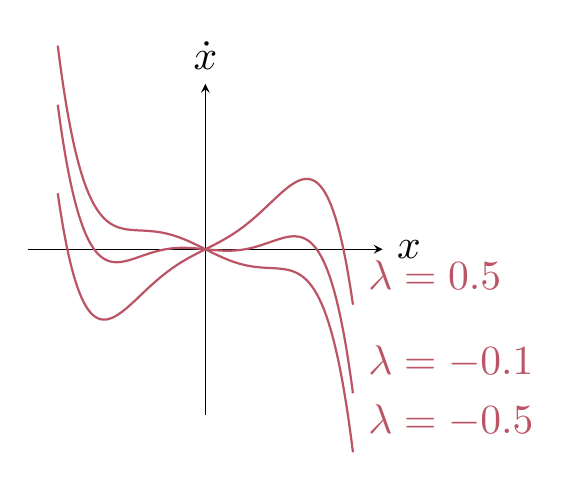
\begin{tikzpicture}[scale=1.5, every node/.style={scale=1.5}]
			\tzaxes(-1.5,-1.4)(1.5,1.4){$x$}{$\dot{x}$}
			\tzfn[col2,thick]{(0.5*\x+\x^3-\x^5)}[-1.25:1.25]{$\la=0.5$ }[ar]
			\tzfn[col2,thick]{(-0.5*\x+\x^3-\x^5)}[-1.25:1.25]{$\la=-0.5$ }[ar]
			\tzfn[col2,thick]{(-0.1*\x+\x^3-\x^5)}[-1.25:1.25]{$\la=-0.1$ }[ar]
			%	\draw [->,thick](0.8,0) -- (0.3,0);
			%	\draw [->,thick](-0.8,0) -- (-0.3,0);
			%	\draw [->,thick](1.2,0) -- (1.5,0);
			%	\draw [->,thick](-1.2,0) -- (-1.5,0);
			%	\node (a) at (0,0) {};
			%	\filldraw (a.center) circle [radius=0.1cm];
			%	\draw (a)+(1,0) circle [radius=0.1cm];
			%	\draw (a)+(-1,0) circle [radius=0.1cm];
		\end{tikzpicture}  \qquad \qquad
		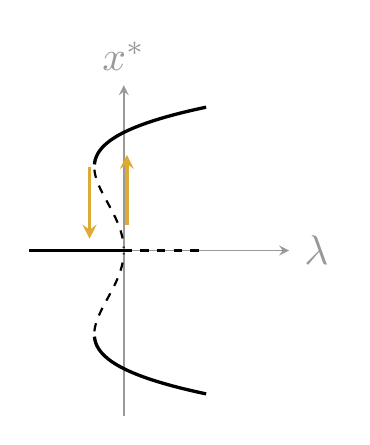
\begin{tikzpicture}[scale=1.5, every node/.style={scale=1.5}]
			%	\tzaxes(-0.5,-2)(2,2){$x$}{$r$}
			\tzfn[black,very thick]{sqrt(0.5)*sqrt(1+sqrt(1+4*\x))}[-0.249:0.7]{}[ar]	
			\tzfn[black, very thick]{-sqrt(0.5)*sqrt(1+sqrt(1+4*\x))}[-0.249:0.7]{}[ar]
			\tzfn[black,dashed,thick]{sqrt(0.5)*sqrt(1-sqrt(1+4*\x))}[-0.249:0]{}[ar]	
			\tzfn[black,dashed,thick]{-sqrt(0.5)*sqrt(1-sqrt(1+4*\x))}[-0.249:0]{}[ar]
			\draw [-,very thick](-0.8,0) -- (0,0);
			\draw [dashed,thick](0,0) -- (0.7,0);
			\draw [->,semithick,opacity=0.4](-0.5,0) -- (1.4,0)  node[right] {$\la$};
			\draw [->,semithick,opacity=0.4](0,-1.4) -- (0,1.4) node[above] {$x^*$} ;
			\draw [col1,->,very  thick](0.026, 0.22) -- (0.026, 0.71 + 0.1);
			\draw [col1,->,very  thick](-0.29, 0.71) -- (-0.29,0.1);
			%			\node (a) at (0,0) {};
			%	\node[circle,draw,minimum size=10cm] (a) at (0,0) {};
			%			\draw (a.center) circle [radius=0.1cm];
			%			\filldraw (a)+(1,0) circle [radius=0.1cm];
			%			\filldraw (a)+(-1,0) circle [radius=0.1cm];
			%	\tzfn'[red,thick]{(\x)^2}[-1:2]{$f^{-1}(x)$}\\[ar] % inverse
		\end{tikzpicture}
	\end{center}
	\caption{Stability of $\dot{x}=\la x+x^3-x^5$. Between $\la=-0.25$ and $\la=0$ the system has three stable branches, while, after $\la=0$ the branch at $x=0$ becomes unstable. This means that in the region  $\la=(-0.25,0)$ the system presents hysteresis. \textcolor{red}{maybe i shuold choose if i keep this or fig 4.2, not both} }
	\label{fig: supercritical pithfork}
\end{figure}


If eq.\eqref{eq: ODES} has a set of equilibria or fixed points \footnote{ $\vec{x}(t)=\vec{x}^*$ such that $\dot{\vec{x}}=0$.  }, $ \left\lbrace \vec{x}^*_1,\dots, \vec{x}^*_k \right\rbrace $, then a Taylor expansion around this points gives 

\begin{equation}
\dot{\vec x}(x\approx x^*,t)\approx \vec f(\vec{x}^*,t)+ \vec{\nabla}  \vec f(\vec{x}^*,t)(\vec{x}-\vec{x}^*)+ \frac{1}{2} \vec{\nabla} \vec{\nabla} \vec f(\vec{x}^*,t)(\vec{x}-\vec{x}^*)^2+\dots 
\label{eq: EWS_taylor}
\end{equation}
where $\vec{x}^*=(x^*_1,\dots,x^*_n)$ is an equilibrium; and  
\begin{equation}
	\vec{\nabla}  \vec f(\vec x^*,t)=M=
	\begin{bmatrix}
		\frac{d f_1}{d x_1}\hdots \frac{d f_1}{d x_n}  \\
		\vdots \\
		\frac{d f_n}{d x_1}\hdots \frac{d f_n}{d x_n}
	\end{bmatrix}
\end{equation}
is the Jacobian of $\vec f$, also called   the linear decay rate (LDR) when $\vec{x}^*(\la)$ is a stable state of the system.
Here we will call $m_j$ the eigenvalues of $M$, and we will call $||M||$  the maximum eigenvalue $m_{max}=\max \left\lbrace m_j \right\rbrace $.
If the system is near a stable equilibrium, and we assume there is a clear separation of scales, that is $||M||$ much larger than the other eigenvalues, then the system is dominated by the slowest timescale (the relaxation time) defined as   
\begin{equation}
	t^*=-\frac{1}{||M(x^*)||}.
\end{equation}

Under this assumptions the system behaves locally as a 1-dimensional system. Therefore we drop the vector notation from now on, unless needed, and we use $M$ and $||M||$ as the same \textcolor{red}{this is not the phrasing you are looking for} .

Since we are close to the stable equilibrium $x^*$, at first order we get 
\begin{equation}
	f|_{x^*}=\cancelto{0}{f(x^*)}+f'(x^*)(x-x^*) \rightarrow \dot{x}|_{x^*}=M(x^*)(x-x^*)
\end{equation}
where the prime denotes differentiation with respect to $x$.

This gives us a local behavior  
\begin{equation}
	x(x\approx x^*)=A e^{M(x^*)t}+x^*
\end{equation}
where $A$ is an integration constant depending on the initial condition. 

We call a co-dimension-1 critical transition, a bifurcation where, as the system approaches a bifurcation point defined by a single control parameter value $\la=\la_c$, the return rate approaches $0$.

\begin{figure}[htb]
	\begin{center}
		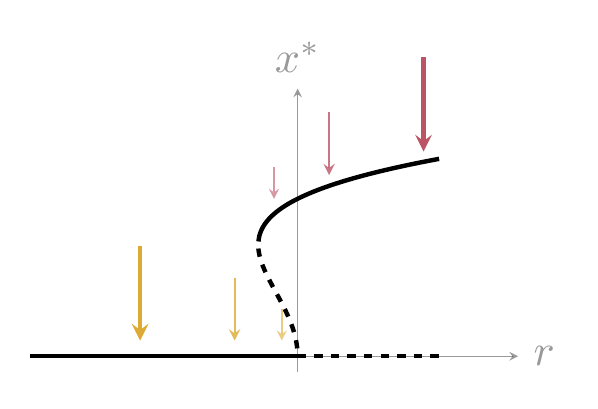
\begin{tikzpicture}[scale=2, every node/.style={scale=1.6}]
			%	\tzaxes(-0.5,-2)(2,2){$x$}{$r$}
			\tzfn[black,ultra thick]{sqrt(0.5)*sqrt(1+sqrt(1+4*\x))}[-0.249:0.9]{}[ar]	
			%		\tzfn[black,ultra thick]{-sqrt(0.5)*sqrt(1+sqrt(1+4*\x))}[-0.249:0.9]{}[ar]
			\tzfn[black,dashed, ultra thick]{sqrt(0.5)*sqrt(1-sqrt(1+4*\x))}[-0.249:0]{}[ar]	
			%	\tzfn[black,dashed,very thick]{-sqrt(0.5)*sqrt(1-sqrt(1+4*\x))}[-0.249:0]{}[ar]
			\draw [-,ultra thick](-1.7,0) -- (0,0);
			\draw [dashed, ultra thick](0,0) -- (0.9,0);
			\draw [->,thin,opacity=0.4](-0.5,0) -- (1.4,0)  node[right] {$r$};
			\draw [->,thin,opacity=0.4](0,-0.1) -- (0,1.7) node[above] {$x^*$} ;
			
			%		\coordinate (c1) at ((0.5^(0.5))*(1+(1+4*0.9)^(0.5))^(0.5));
			
			\draw [->,ultra thick,col1](-1, 0.7) -- (-1, 0.1);
			\draw [->,col1,thick, opacity=0.8](-0.4, 0.5) -- (-0.4,  0.1);
			\draw [->,col1,semithick, opacity=0.6](-0.1, 0.3) -- (-0.1,  0.1);
			
			\draw [->,ultra thick,col2](0.8, 1.9) -- (0.8,  1.9-0.6);
			\draw [->,col2,thick, opacity=0.8](0.2, 1.55) -- (0.2,  1.55-0.4);
			\draw [->,col2,semithick, opacity=0.6](-0.15, 1.2) -- (-0.15,  1.2-0.2);
			%			\node (a) at (0,0) {};
			%	\node[circle,draw,minimum size=10cm] (a) at (0,0) {};
			%			\draw (a.center) circle [radius=0.1cm];
			%			\filldraw (a)+(1,0) circle [radius=0.1cm];
			%			\filldraw (a)+(-1,0) circle [radius=0.1cm];
			%	\tzfn'[red,thick]{(\x)^2}[-1:2]{$f^{-1}(x)$}\\[ar] % inverse
		\end{tikzpicture}
	\end{center}
	\caption{Relaxation time changes approaching the bifurcation, pictured by the thickness of the arrows in each stable branch. \textcolor{red}{it would be better with a cool/warm colormap for stable/unstable and real values.} }
	\label{fig: relax time.}
\end{figure}

Critical slowing down (CSD) is the slowing down of relaxation times near a stable solution when the system is near a bifurcation. In other words, it is the loss of resilience of the stable manifold near a transition. 

This is usually pictured as the potential of a system with enough damping to have overdamped solutions, defined as $V=-\int dx\,f(x,\la)$. In this picture, as the system approaches the bifurcation, it looses stability (the potential well becomes more shallow \footnote{It might also become more narrow, in which case the tipping might also happen due to a change in the basin. Though we do not focus on this cases.} ) which means a perturbation might send the system to another stable state, as pictured in figure \ref{fig: resiliance_and_csl}.


\begin{figure}[htbp]
	\begin{center}
		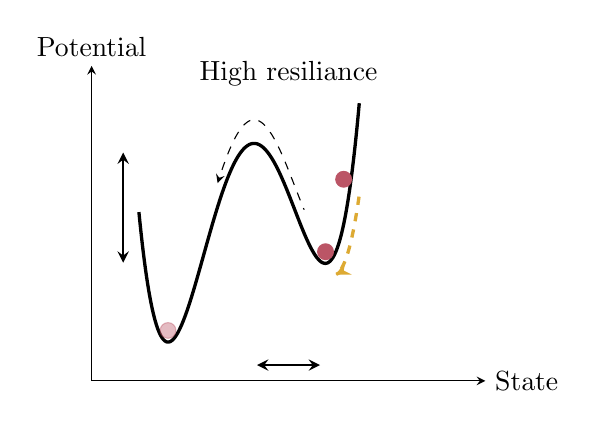
\begin{tikzpicture}
			\tzaxes(0,0)(5,4){State}{Potential}
			\tzfn[black,very thick]{2*(\x-1)^2*(\x-3)^2+0.5*\x}[0.6:3.4]{ }[ar]
			\tzfn[<-,black,dashed]{2*(\x-1)^2*(\x-3)^2+0.5*\x+0.3}[1.6:2.7]{ }[ar]
			\tzfn[<-,very thick,col1,dashed]{2*(\x-0.2-1)^2*(\x-0.1-3)^2+0.5*(\x-0.2)-0.1}[3.1:3.4]{ }[ar]
			%			\draw [->,thick](0.8,0) -- (0.3,0);
			%			\draw [->,thick](-0.8,0) -- (-0.3,0);
			%			\draw [->,thick](1.2,0) -- (1.5,0);
			%			\draw [->,thick](-1.2,0) -- (-1.5,0);
			\node (a) at (0,0) {};
			\filldraw [col2,opacity=0.4] (0.97,0.5+0.14) circle [radius=0.1cm];
			\filldraw [col2](2.97,1.5+0.14) circle [radius=0.1cm];
			\filldraw [col2](3.2, 2.06 + 0.5) circle [radius=0.1cm];
			\draw [<->,thick](0.4,1.5)--(0.4,2.9);
			\draw [<->,thick](2.1,0.2)--(2.9,0.2);
			\node (t) at (2.5,3.9) {High resiliance}[c];		
		\end{tikzpicture} 
		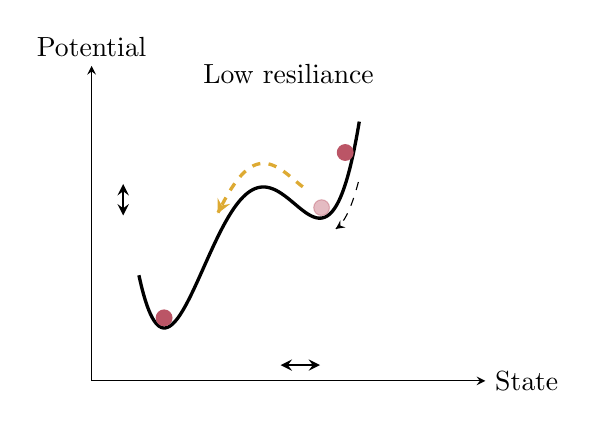
\begin{tikzpicture}
			\tzaxes(0,0)(5,4){State}{Potential}
			\tzfn[ black,very thick]{(\x-1)^2*(\x-3)^2+0.7*\x}[0.6:3.4]{ }[ar]
			\tzfn[<-,very thick,col1,dashed]{(\x-1)^2*(\x-3)^2+0.7*\x+0.3}[1.6:2.7]{ }[ar]
			\tzfn[<-,black,dashed]{(\x-0.2-1)^2*(\x-0.1-3)^2+0.7*(\x-0.2)-0.1}[3.1:3.4]{ }[ar]
			%			\draw [->,thick](0.8,0) -- (0.3,0);
			%			\draw [->,thick](-0.8,0) -- (-0.3,0);
			%			\draw [->,thick](1.2,0) -- (1.5,0);
			%			\draw [->,thick](-1.2,0) -- (-1.5,0);
			\node (a) at (0,0) {};
			\filldraw [col2] (0.92,0.7+0.1) circle [radius=0.1cm];
			\filldraw [col2,opacity=0.4](2.92,3*0.7+0.1) circle [radius=0.1cm];
			\filldraw [col2] (3.22, 2.4 + 0.5) circle [radius=0.1cm];
			\draw [<->,thick](0.4,2.1)--(0.4,2.5);
			\draw [<->,thick](2.4,0.2)--(2.9,0.2);
			\node (t) at (2.5,3.9) {Low resiliance}[c];		
		\end{tikzpicture}
	\end{center}
	\caption{As the system (left panel) moves closer to a tipping point, it losses resilience (right panel), and the system might change state (red circle) due to a perturbation that was not enough to force the system to tip to a new equilibrium when it had more resilience.    }
	\label{fig: resiliance_and_csl}
\end{figure}

At the same time as the LDR goes to $0$ as shown in figure \ref{fig: relax time.}, the relaxation time increases, which leads to a slowing down of the dynamics(critical slowing down). 
This means that, in the presence of noise (perturbations), the CSD is manifested as an increase of variance.  
%\begin{figure}
%	\centering
%\begin{tikzpicture}
%	\tzaxes(-0.4,-0.5)(2,3){$x$}{$\dot{x}$}
%	\tzfn[blue,thick]{2*(\x)*(\x-1)^2+0.3}[-0.3:1.5]{$f(x)$}[ar]
%	\draw [->,thick](-0.3,0) -- (-0.6,0);
%	\draw [->,thick](-0.3,0) -- (0.3,0) ;
%	\node (a) at (0,0) {};
%	%	\node[circle,draw,minimum size=10cm] (a) at (0,0) {};
%	\filldraw (a)+(-0.4,0) circle [radius=0.1cm];
%	%	\tzfn'[red,thick]{(\x)^2}[-1:2]{$f^{-1}(x)$}\\[ar] % inverse
%\end{tikzpicture}
%	\caption{Slowing down from ghosting. .. dunno if i should keep this. }
%\label{fig: ghosting}
%\end{figure}






\subsection{Estimation for linearly stable systems in critical bifurcations}
\textcolor{red}{by this i mean bifurcation where the eigenvalue is real}

In particular, if the system is linearly stable, then near the stable point, the system returns as

\begin{equation}
	x(t)=Ae^{-M t}+x^*
\end{equation}

For this, we have to ask for the determinant of the jacobian matrix to be non zero, 
\begin{equation}
	det(M(x^*,\lambda))\neq0
\end{equation}

with $\lambda\neq \lambda_c$. Then, we can do a Taylor expansion of the Jacobian near (before) the bifurcation. 
If the eigenvalues are real,  at the bifurcation the determinant becomes zero and we get:
\begin{equation}
	M(x^*,\la\approx \lambda_c)\approx \cancelto{0}{M(x^*,\lambda_c)}+\partial_\lambda M(x^*,\lambda_c) (\lambda-\lambda_c)+\frac{1}{2}\partial^2_\lambda M(x^*,\lambda_c) (\lambda-\lambda_c)^2+... 
\end{equation}

Thus, near a bifurcation we expect the return time to be 
\begin{equation}
	t^*=-\frac{1}{M}\approx \frac{\kappa_1}{(\lambda-\lambda_c)}+\frac{\kappa_2}{(\lambda-\lambda_c)^2}+\dots
\end{equation}
where $\kappa_j$ are constants related to the different derivatives $\partial^j_\lambda M(x^*,\lambda_c)$.

Therefore, before the bifurcation, the return rate goes as  $1/(\lambda-\lambda_c)$ and as the system gets closer to the bifurcation the higher order terms dominate the return time which diverges geometrically at the bifurcation\footnote{\textcolor{red}{I could think of an example where this coefficients are all $1$ and it gives an exponential series.}}.

% $1/(\lambda-\lambda_c)^n$ and the return time 

\section{Types of tipping}

If we say a system tips when it changes some aspect of its behavior, dynamical systems can display several kind of tipping\footnote{It should be noted that we do not explore bifurcations of the basins of attraction.}.

We can classify this changes according to the mechanism that forces the system to change. This could be because:
\begin{enumerate}
	\item the system crosses a dynamical bifurcation (B-tipping)
	\item   the noise is large enough for the system to be able to reach  the basin of another regime (N-tipping)
	 \item  a parameter is the system is also evolving in time, and this forces the system to either have a new dynamical equilibrium or to tip towards another regime depending on the rate of change of the parameter (R-tipping)
	 \item to external shocks that forces the system to another basin (S-tipping).
\end{enumerate} 

\begin{figure}[htb]
	\centering
	Tipping points
	\hline
	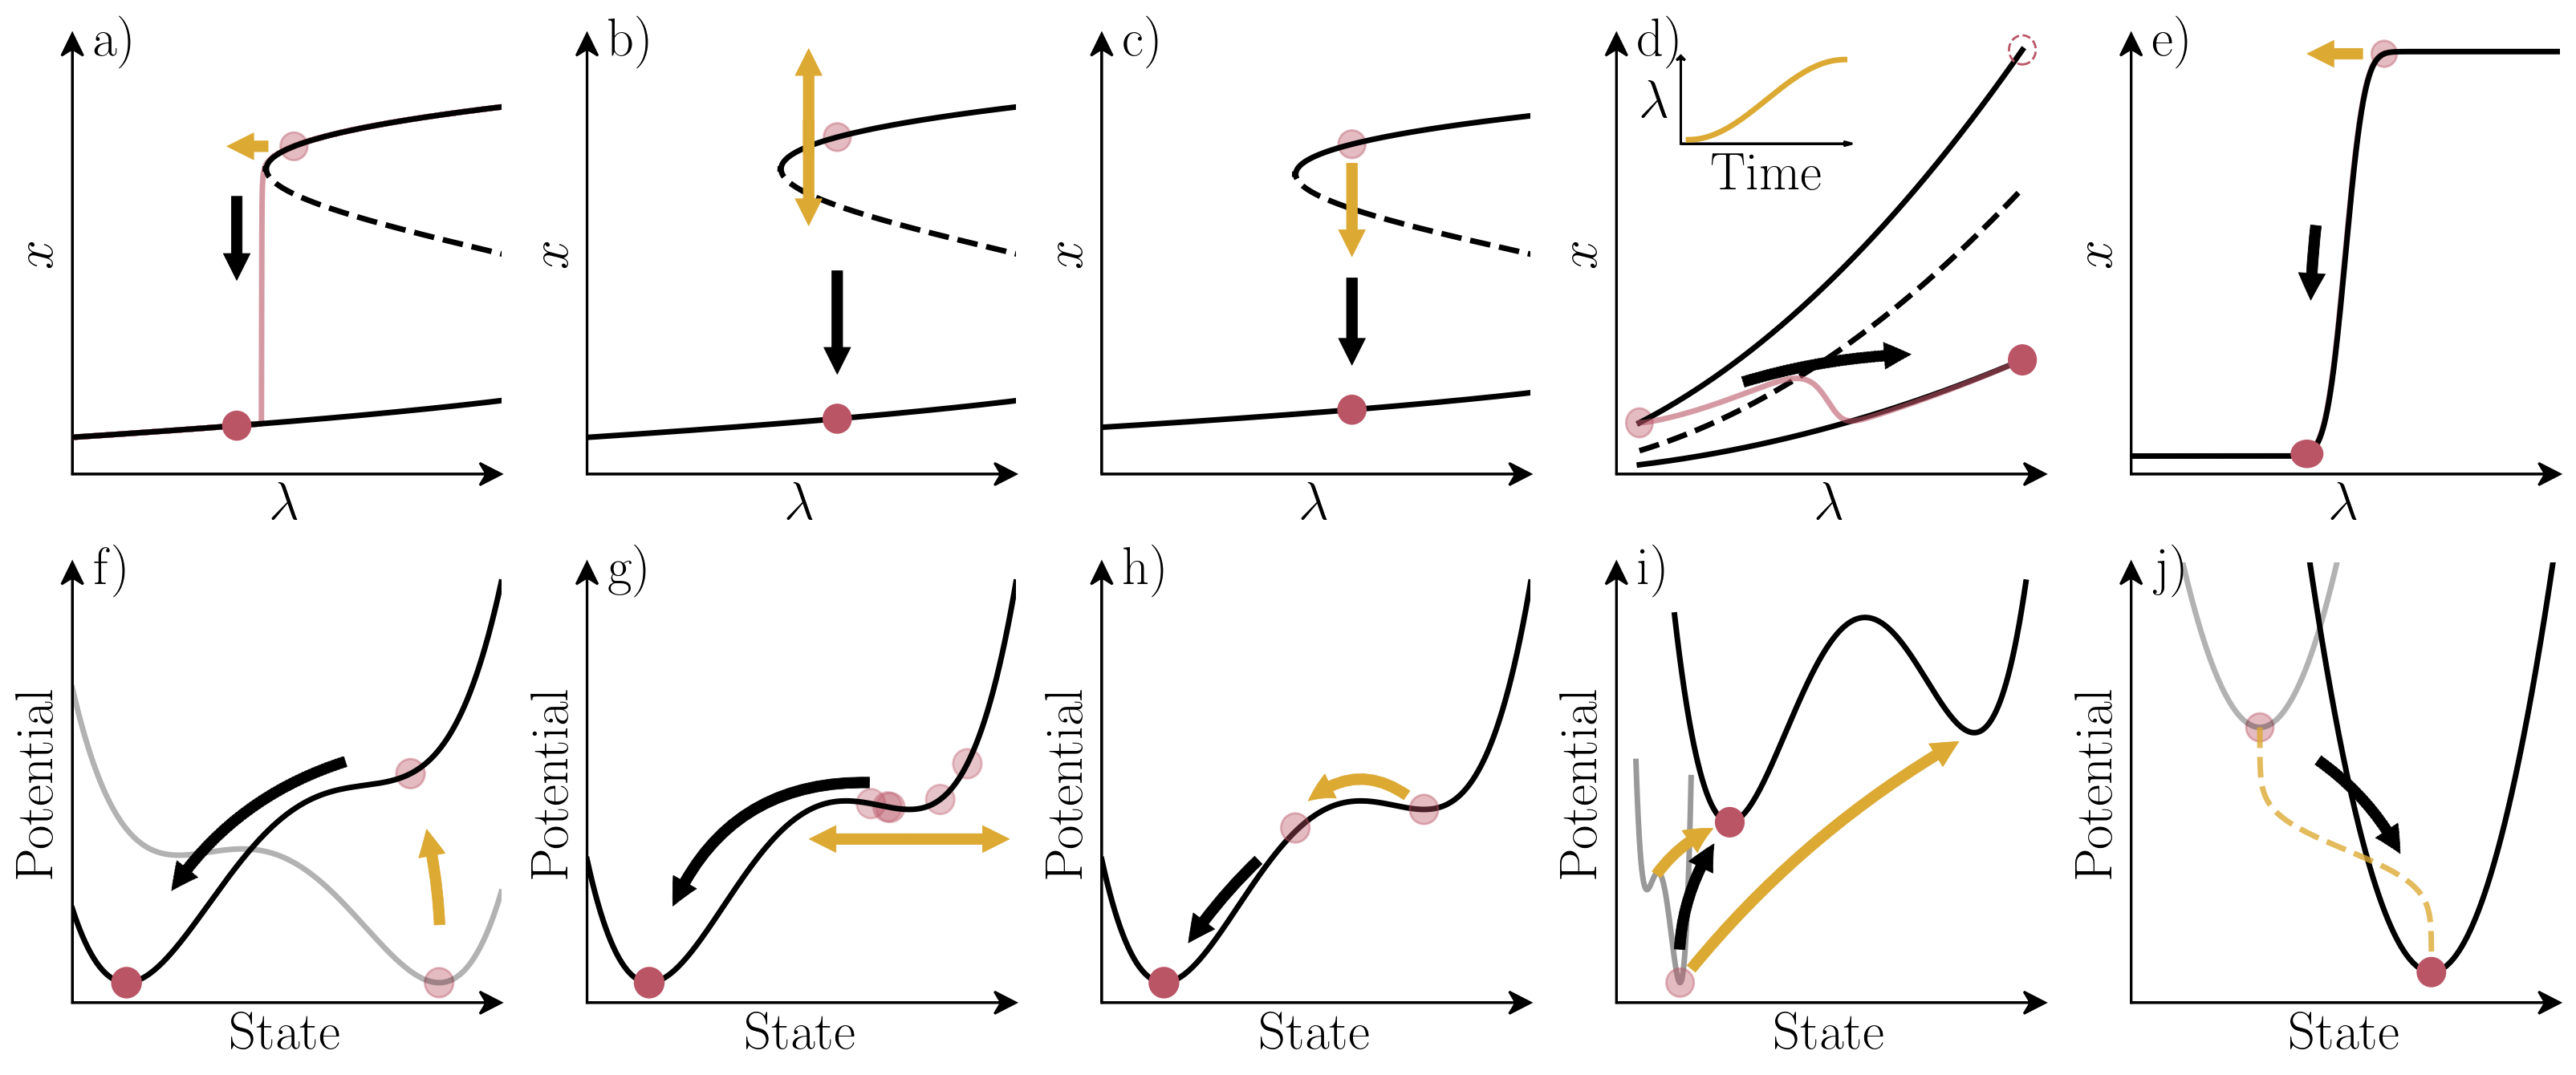
\includegraphics[width=1\linewidth]{Images/Metrics/tippings}
	\caption{Top row shows the effect of the tipping on the bifurcation diagram, while bottom row shows the corresponding potential picture. a, f) Tipping due to bifurcation (B-tipping). b, g) Tipping due to  noise (N-tipping). e, h) Tipping due to a single large perturbation (S-tipping). d, i) Tipping due to a quick change in control parameter (R-tipping). e, j) Tipping due to a fast change in the stable state (quick transition). }
	\label{fig:largetippingsscheffer}
\end{figure}


\subsection{Dynamical bifurcations, or B-tipping}
Following \cite{Thompson2011a}, we can classify codimension-1 bifurcations\footnote{Bifurcations that can be encountered when sweeping or scanning only one control parameter.} on how much the system changes and how hard it is to reverse the system to the previous regime. 
Taking this into account we can  classify them into safe (\cref{tab:safe_bifs}), dangerous (\cref{tab:explos_bifs}), and explosive bifurcations\footnote{Here there might be a few new bifurcations missing...}  (\cref{tab:dangerous_bifs}).


\begin{table}[H]
			\centering
		\begin{tabular}{ll}
			\hline
			\multicolumn{2}{c}{\textbf{Safe bifurcations}} \\
			\textbf{a) Local Supercritical bifurcations} & \\
				1. Supercritical Hopf & Point to cycle\\
				2. Supercritical Neimark-Sacker (secondary Hopf) & Cycle to torus \\				
				3. Supercritical Flip/period doubling & Cycle to cycle \\			
			\textbf{b) Global bifurcations} & \\
				1. Band Merging & Chaos to chaos\\
	& \\
		\multicolumn{2}{c}{Features}	\\
		\multicolumn{2}{l}{\textbf{Subtle:} continuous supercritical growth of the new attractor path}\\
		\multicolumn{2}{l}{	\textbf{Safe:} no fast jump or enlargement of the attracting set }	\\
		\multicolumn{2}{l}{	\textbf{Determinate:} single outcome even with small noise}	\\
		\multicolumn{2}{l}{	\textbf{No hysteresis:} path retraced on reversal of control sweep}	\\
		\multicolumn{2}{l}{	\textbf{No basin change:} basin boundary remote from attractors}\\
		\multicolumn{2}{l}{	\textbf{No intermittency:} in the responses of the attractors}	\\   
	\hline
			\end{tabular}
			\caption{Safe bifurcations. These include supercritical forms of the local bifurcations and the less well-known global 'band merging'. Taken from \cite{Thompson2011a}.  }
			\label{tab:safe_bifs}
\end{table}

It should be noted that the definition of \textit{safe} being ``no fast jump or enlargement of the attracting set'' where fast jump implies a discontinuity of the stable sets (like in a saddle-node bifurcation). Thus the case where the system performs a smooth yet large transition for a small shift on the parameters (as shown in figure \ref{fig:largetippingsscheffer} e,j)) is not excluded, which implies that there is also no critical slowing down to give warning. 
%Therefore this definition of safe is good regarding the universal mechanisms of the bifurcations (the normal forms close to the bifurcations, or the topology), but in particular applications this might still be considered dangerous. In particular if this big transition is not a real dynamical bifurcation but just an intense dependence con the control parameters as in this case 






\begin{table}[H]
				\centering
	\begin{tabular}{ll}
		\hline
		\multicolumn{2}{c}{\textbf{Dangerous bifurcations}} \\
		\textbf{a) Local saddle-node bifurcations} & \\
		1. Static Fold (saddle-node of fixed point) & From point\\
		2. Cyclic Fold (saddle-node of Cycle) & From Cycle\\				
		\textbf{a) Local subcritical bifurcations} & \\
		1. Subcritical Hopf  & From point\\
		2. Subcritical Neimark-Sacker (secondary Hopf)  & From Cycle\\		
		3. Subcritical flip (Period doubling)  & From Cycle\\				
		\textbf{c) Global bifurcations} & \\
		1. Saddle connection (homoclinic connection) &  From Cycle\\
		2. Regular-saddle catastrophe (boundary crisis) &  From Chaos\\
		3. Chaotic-saddle catastrophe (boundary crisis) &  From Chaos\\
		& \\
		\multicolumn{2}{c}{Features}	\\
		\multicolumn{2}{l}{\textbf{Catastrophic:} sudden disappearance of attractor}\\
		\multicolumn{2}{l}{	\textbf{Dangerous:} Sudden jump to new attractor }	\\
		\multicolumn{2}{l}{	\textbf{Indeterminacy:} outcome can depend on global topology}	\\
		\multicolumn{2}{l}{	\textbf{hysteresis:} path not reinstalled on reversal of control sweep}	\\
		\multicolumn{2}{l}{	\textbf{Basin change:} Tends to zero (b), attractor hits edge of residual basin (a,c)}\\
		\multicolumn{2}{l}{	\textbf{No intermittency:} but critical slowing in global events}	\\   
		\hline
	\end{tabular}
	\caption{Dangerous bifurcations. Taken from \cite{Thompson2011a}. }
	\label{tab:dangerous_bifs}
\end{table}



\begin{table}[H]
	\centering
	\begin{tabular}{ll}
		\hline
		\multicolumn{2}{c}{\textbf{Explosive bifurcations}} \\
		
		1. Flow explosion (omega explosion, SNIPER) & Point to cycle\\
		2. Map explosion (omega explosion, mode locking) & Cycle to torus \\				
		3. Intermittency explosion: Flow & Point to chaos \\			
		4. Intermittency explosion: Map (temporal intermittency) & Cycle to chaos \\	
		5. Regular-Saddle explosion (interior crisis) & Chaos to chaos \\	
		6. Chaotic-Saddle explosion (interior crisis) & Chaos to chaos \\	
		& \\
		\multicolumn{2}{c}{Features}	\\
		\multicolumn{2}{l}{\textbf{Catastrophic:} global events, abrupt enlargement of attracting set}\\
		\multicolumn{2}{l}{	\textbf{Explosive:} enlargement, but no jump to remote attractor}	\\
		\multicolumn{2}{l}{	\textbf{Determinate:} single outcome even with small noise}	\\
		\multicolumn{2}{l}{	\textbf{No hysteresis:} path retraced on reversal of control sweep}	\\
		\multicolumn{2}{l}{	\textbf{No basin change:} basin boundary remote from attractors}\\
		\multicolumn{2}{l}{	\textbf{Intermittency:} lingering in old domain, flashes through the new}	\\   
		\hline
	\end{tabular}
	\caption{Explosive bifurcations. Taken from \cite{Thompson2011a}.}
	\label{tab:explos_bifs}
\end{table}


For \textit{dangerous} bifurcations, a recent distinction by \cite{Ritchie2021} becomes relevant for some kinds of bifurcations where the control parameter is changed very fast. In this case, it is possible to avoid a full tipping of the system if the parameter is also reversed fast enough, as shown in  \cref{fig:overshootsaving}. 
This means that it would be relevant to distinguish fast and slow tippings to classify cases in which it is possible to 'save' the system from a dangerous bifurcation even after it happened. 

%\begin{figure}
%	\centering
%	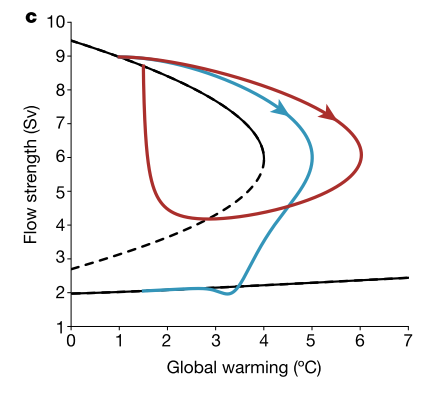
\includegraphics[width=0.7\linewidth]{Images/Metrics/overshoot_saving}
%	\caption{Example of a system avoiding full tipping, taken from \citep{Ritchie2021}. In this case the temperature grows very fast until $6$~C and then quickly goes back to $1.5$~C.As the temperature grows both the blue trajectory (slow forcing) and the red trajectory (fast forcing) go trough the bifurcation threshold. However the red trajectory manages to recover from the tipping thanks to the faster parameter change.}
%	\label{fig:overshootsaving}
%\end{figure}


\begin{figure}
	\centering
	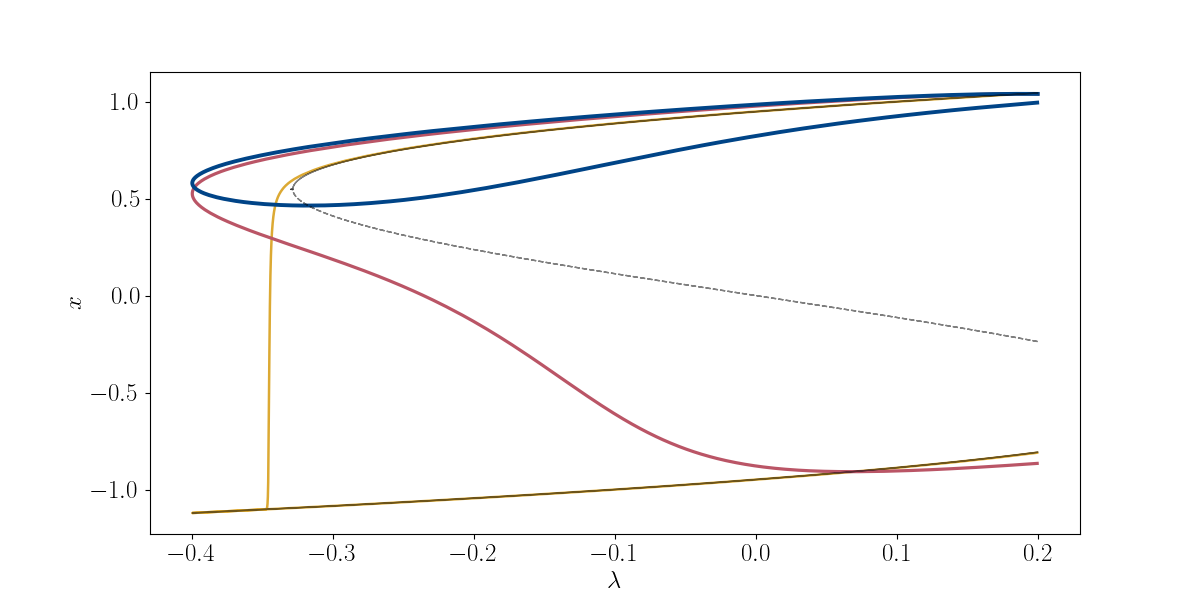
\includegraphics[width=0.9\linewidth]{Images/Metrics/overshoot2}
	\caption{Example of a system avoiding full tipping, inspired by \cite{Ritchie2021}, where a system's control parameter is swiped from an initial value, past a bifurcation value, and then is set back to the initial value.  In this case the yellow trajectory represents a slow sweeping of the control parameter, the red trajectory represents an intermediate sweeping speed where the system still tips, and the blue trajectory presents a fast sweep where the systems avoids tipping to the lower stable branch.   }
	\label{fig:overshootsaving}
\end{figure}



% 
%\begin{figure}[htp]
%	\centering
%	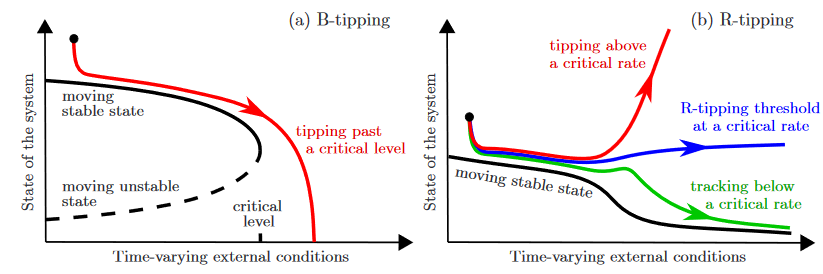
\includegraphics[width=0.9\linewidth]{Images/Metrics/exampl}
%	\caption{..}
%	\label{fig:exampl}
%\end{figure}

%
%\begin{figure}[htbp]
%	\begin{center}
%		\begin{tikzpicture}
%			\tzaxes(0,0)(5,4){State}{Potential}
%			\tzfn[black,line width=0.2mm,col1,opacity=0.4]{2*(\x-1)^2*(\x-3)^2+0.5*\x+0.03}[0.6:3.4]{ }[ar]
%			\tzfn[black, thick]{2*(\x-1)^2*(\x-3)^2+0.5*\x}[0.6:3.4]{ }[ar]
%		%	\tzfn[<-,black,dashed]{2*(\x-1)^2*(\x-3)^2+0.5*\x+0.3}[1.6:2.7]{ }[ar]
%		%	\tzfn[<-,very thick,col1,dashed]{2*(\x-0.2-1)^2*(\x-0.1-3)^2+0.5*(\x-0.2)-0.1}[3.1:3.4]{ }[ar]
%			%			\draw [->,thick](0.8,0) -- (0.3,0);
%			%			\draw [->,thick](-0.8,0) -- (-0.3,0);
%			%			\draw [->,thick](1.2,0) -- (1.5,0);
%			%			\draw [->,thick](-1.2,0) -- (-1.5,0);
%			\node (a) at (0,0) {};
%			\filldraw [col2,opacity=0.4] (0.97,0.5+0.14) circle [radius=0.1cm];
%			\filldraw [col2](2.97,1.5+0.14) circle [radius=0.1cm];
%			\filldraw [col2](3.2, 2.06 + 0.5) circle [radius=0.1cm];
%		%	\draw [<->,thick](0.4,1.5)--(0.4,2.9);
%		%	\draw [<->,thick](2.1,0.2)--(2.9,0.2);
%		%	\node (t) at (2.5,3.9) {High resiliance}[c];		
%		\end{tikzpicture} 
%		\begin{tikzpicture}
%			\tzaxes(0,0)(5,4){State}{Potential}
%
%			\tzfn[black,ultra thick,col1]{2*(\x-1)^2*(\x-3)^2+0.5*\x+0.01}[0.6:3.4]{ }[ar]
%			\tzfn[black, thick]{2*(\x-1)^2*(\x-3)^2+0.5*\x}[0.6:3.4]{ }[ar]
%			%			\draw [->,thick](0.8,0) -- (0.3,0);
%			%			\draw [->,thick](-0.8,0) -- (-0.3,0);
%			%			\draw [->,thick](1.2,0) -- (1.5,0);
%			%			\draw [->,thick](-1.2,0) -- (-1.5,0);
%			\node (a) at (0,0) {};
%			\filldraw [col2] (0.92,0.7+0.1) circle [radius=0.1cm];
%			\filldraw [col2,opacity=0.4](2.92,3*0.7+0.1) circle [radius=0.1cm];
%			\filldraw [col2] (3.22, 2.4 + 0.5) circle [radius=0.1cm];
%		%	\draw [<->,thick](0.4,2.1)--(0.4,2.5);
%		%	\draw [<->,thick](2.4,0.2)--(2.9,0.2);
%		%	\node (t) at (2.5,3.9) {Low resiliance}[c];		
%		\end{tikzpicture}
%	\end{center}
%	\caption{As the system(ball)  }
%	\label{fig: rate_intertial_picture}
%\end{figure}


%\input{Chapters/EWS_rate_tikz.tex}

%
%\begin{figure}[H]
%	\centering
%	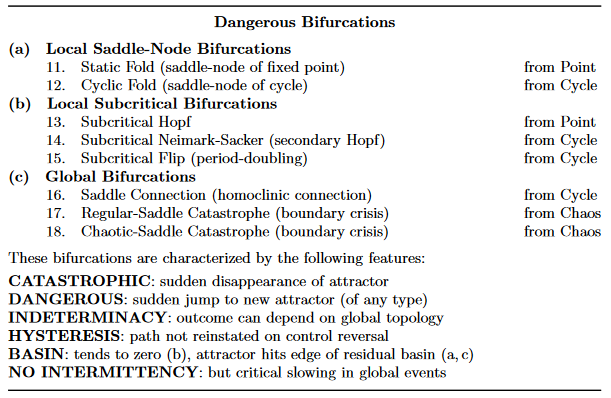
\includegraphics[width=0.9\columnwidth]{Images/Metrics/catastrofic_bifurc.png}
%	\caption{Dangerous bifurcations}
%	%	\caption{Events per ms}
%	\label{tab:dangerous_bifs}
%\end{figure}

Table \ref{tab:codim_1_prec} shows a list of possible precursors to  codimension-1 bifurcations. 

\begin{table}[H]
				\centering
	\begin{tabular}{lll}
		\hline
		\multicolumn{3}{c}{\textbf{Precursors of Codimension-1 Bifurcations }} \\
		Supercritical Hopf & S: point to cycle & LDR$\rightarrow 0$ linearly with control \\
		Supercritical Neimark & S: point to torus & LDR$\rightarrow 0$ linearly with control \\
		Supercritical flip & S: cycle to cycle & LDR$\rightarrow 0$ linearly with control \\
		Band merging & S: chaos to chaos & Separation decreases linearly \\
		Flow explosions & E: point to cycle & Path folds. LDR$\rightarrow 0$ linearly with control \\
		Map explosion & E: cycle to torus & Path folds. LDR$\rightarrow 0$ linearly with control \\
		Intermittency expl: flow & E: point to chaos & LDR$\rightarrow 0$ linearly with control \\
		Intermittency expl: map & E: cycle to chaos & LDR$\rightarrow 0$ as trigger \\
		Regular interior crisis & E: chaos to chaos & Lingering near impinging saddle cycle \\
		Chaotic interior crisis & E: chaos to chaos & Lingering near impinging saddle cycle \\
		Static fold & D: from point & Path folds. LDR$\rightarrow 0$ linearly with control  \\
		Cyclic fold & D: from cycle & Path folds. LDR$\rightarrow 0$ linearly with control \\
		Subcritical Hopf & D: from point & LDR$\rightarrow 0$ linearly with control \\
		Subcritical Neimark & D: from cycle & LDR$\rightarrow 0$ linearly with control \\
		Subcritical glip & D: from cycle & LDR$\rightarrow 0$ linearly with control \\
		Saddle connection & D: from cycle & Period of cycle tends to infinity \\
		Regular exterior crisis & D: from chaos & Lingering near impinging saddle cycle \\
		Chaotic exterior crisis & D: from chaos & Lingering near impinging accessible saddle \\
		\hline
	\end{tabular}
	\caption{Taken from \cite{Thompson2011a}.  }
	\label{tab:codim_1_prec}
\end{table}

%
%\begin{figure}[H]
%	\centering
%	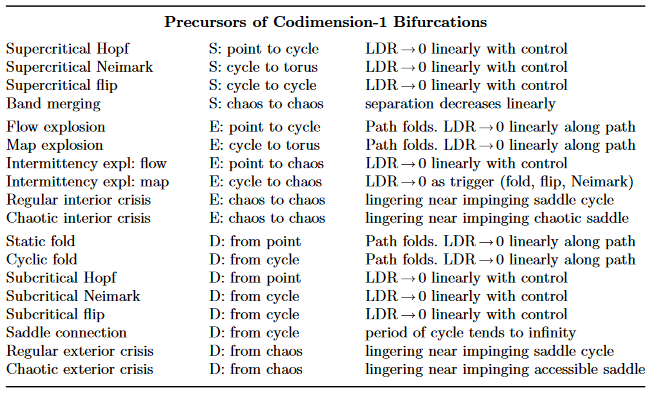
\includegraphics[width=0.9\columnwidth]{Images/Metrics/codim_1_precursors.png}
%	\caption{ safe bifurcations}
%	%	\caption{Events per ms}
%	\label{tab:codim_1_prec}
%\end{figure}

For now we will focus on codimension-1 parameters where the local Local Decay Rate (LDR) approaches 0, and situations where the system goes from a stable state to another. 




%\begin{figure}[hbtp]
%	\centering
%	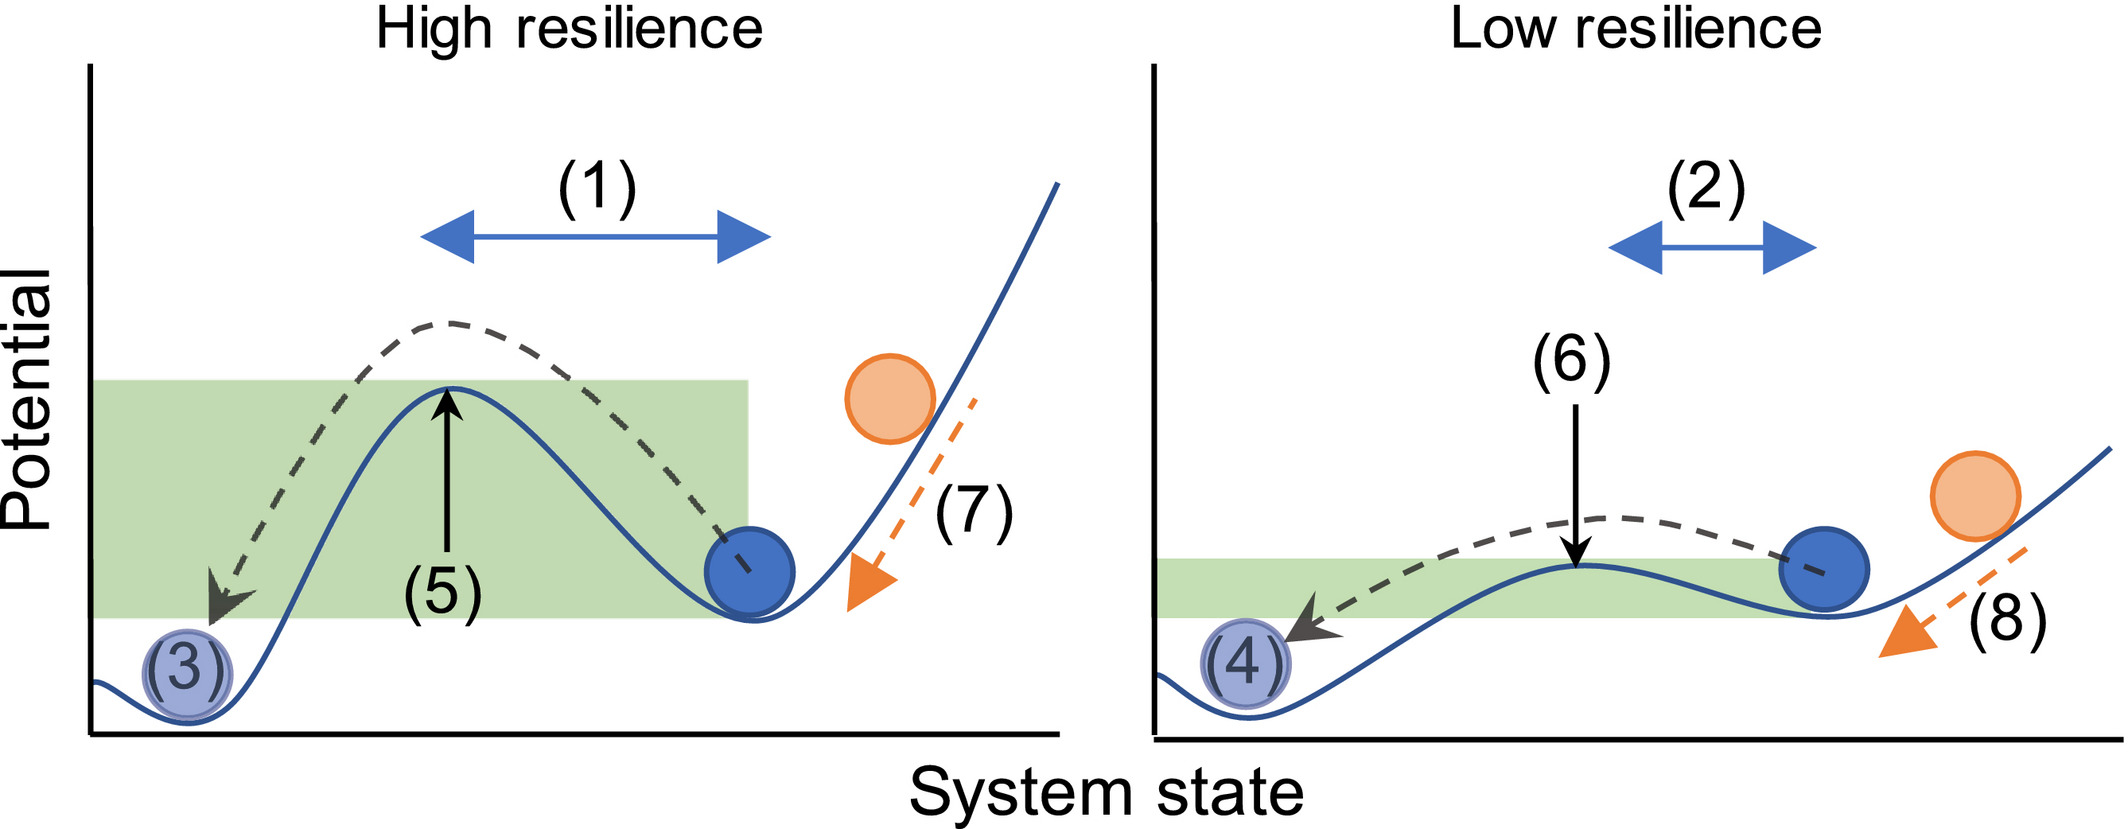
\includegraphics[width=.8\textwidth]{Images/Metrics/resiliance}
%	\caption{Resiliance figure from \cite{Clements2018a} }
%	\label{fig: resiliance}
%\end{figure}



%We can give an easy quantification of this for bifurcation where the eigenvalues are real and there is a change of sign\footnote{For complex valued bifurcations, like the Hopf bifurcation, a threshold timescale could be the slowest timescale of the cycle, or just the period}. 



%If the system is near en equilibrium and is perturbed by white noise with variance $\sigma$, then we can consider a perturbation of $2\sigma$, linearize about the stable state before the transition and estimate the relaxation time. 


%In this case $\dot{x}=f(x)=r(x-2)(x-1)(x-3)$, we linearize about $x=x^*=2$, and use an initial value $x_0=x^*\pm2\sigma=2\pm 2\sigma$.
%\begin{equation}
%	f|_{x^*}=f(x^*)+f'(x^*)(x-x^*) \rightarrow \dot{x}|_{x^*}=f(x^*)+f'(x^*)(x-x^*)
%\end{equation}
%then 
%
%\begin{equation}
%	x|_{x^*+2\sigma}=A e^{f'(x^*+2\sigma)t}+\frac{f(x^*+2\sigma)-f'(x^*+2\sigma)(x^*+2\sigma)}{f'(x^*+2\sigma)}
%\end{equation}
%
%so the characteristic timescale is $t^*=-\frac{1}{f'(x^*+2\sigma)}$.



%In this case the second term is related to the equilibrium, and it is exactly the equilibrium in the $\sigma\rightarrow 0$ limit. 
%This is irrelevant for our analysis, however is it worth noting that, if the analysis is valid, the equilibrium is decoupled (?) from the noise.


%
%Clearly this approximation breaks near the bifurcation since the system cannot be linearized, and the relaxation time goes diverges. However, according to this, the relaxation time is smaller with larger noise. 



%In general, in $n$ dimentions:

%\begin{equation}
%\begin{bmatrix}
%	x_1 \\
%	\vdots \\
%	x_n 
%\end{bmatrix}
%=
%\begin{bmatrix}
%	f_1(x_1, \hdots ,x_n) \\
%	\vdots \\
%	f_n(x_1, \hdots ,x_n)
%\end{bmatrix}
%\end{equation}

%Now we will have $n$ relaxation times given by the eigenvalues ($m_n$) of the Jacobian of the system.


%
%Then the relaxation time-scale is the slowest timescale, given by the dominant eigenvalue $m_{max}$.
%
%\begin{equation}
%	 t^*=-\frac{1}{m_{max}(\vec{x}^*)}
%\end{equation}

\subsection{Pure stochastic tipping, or N-tipping}

In this case there is no need for a changing parameter, we consider the system at a given value of the control $\la_0$, with stable equilibrium $x^*$  and respective basin of attraction ($\mathcal{B}(x^*)$). If this system has a noise with a standard deviation ($\mathrm{STD}(x)$), then there is a non zero probability for the system to escape the basin, or alternatively, an average escape time. 

%For additive noise, the system can be written as a Langevin equation 

If the local stable attractor has a local potential well with the smallest well height being $\Delta U$, then the  escape time is approximated by Kramers time: 
\begin{equation}
	t_k=c e^{2\Delta U/\mathrm{Var}^2}
\end{equation} 
Where Var denotes the variance of the system around $x^*$.

%There have been accounts \citep{bibid} where the importance of the noise to signal ratio is remarked for the performance of EWS. 
%This seems to point that this is not important and the relevant feature is the relation between the noise and the local landscape of the manifold, through the relaxation timescale. This is further evident when we consider we can translate the whole problem to whichever value we want\footnote{for example at $0$ ( $\dot{x}=f(x)=\la(x-1)(x)(x+1)$)}, then the signal to noise ratio for the stable point at the middle is infinite, but the normal form of the equation and all the dynamics remain the same. 

It should be noted that translations of the dynamical system work differently for additive or multiplicative noise.  
If a 1D system\footnote{Also true in higher dimension, but in 1D the states are ordered.} has two stable states for a given parameter ($x_+^*>x_-^*$) with additive noise of intensity $\sigma$ then all probabilities and dynamics are the same if translated\footnote{$dx=f(x,\la)\, dt+ \sigma dW$ and $dx=f(x+\mu,\la)\, dt+ \sigma dW$  have the same statistical properties.} to ($x_+^*+\mu>x_-^*+\mu$). 

However with multiplicative noise, translating the system not only changes the noise, but the probabilities of escaping from each well. A system with a state at $x_+=2$ has twice the noise of the state at  $x_-=1$, however it will have almost the same noise if translated to  $x_+=22$ and $x_-=21$.

Some works related to noise tipping can be found in \citep{Sharma2015}.

In this case the tipping cannot be predicted since it is the result of a purely random  process, however the probability of tipping can be studied.






\subsection{Rate induced bifurcations, or R-tipping}

Following the work done by \cite{Ashwin2012,Kees2017a,Kiers2020a}, if we consider a control parameter that changes with time $\la=\la(t)$ then the system of equations \eqref{eq: ODES} becomes a  non-autonomous system. 
Now the full dynamical system can be written as
\begin{equation}
	\begin{cases}
		d x&=f(x,\lambda) \, dt\\
		d \lambda&= c_\lambda(t,\la)\, dt
	\end{cases}
\label{eq:Aug1}
\end{equation}
which we call the augmented system of  equation \eqref{eq: ODES}.
 $c_\lambda(t,\la)$ is a $C^0$ function that does not depend on $x$. 
If $c_\lambda(t,\la) \neq 0$ this variable does not have a nullcline, therefore there  are no equilibria. However, we can study if the system can track the equilibrium of the autonomous system as the control parameter changes. 
In particular, we want to know for which parameter speeds the system can 'close track'  the autonomous equilibrium $x^*(\la)$. 

In this case, close tracking $x^*$ implies that the trajectories of the augmented system \cref{eq:Aug1}, also called pullback attractor $X(t)$,  are bounded around the expected equilibrium, that is $|X(t)-x^*(t)|<\epsilon$. 

In \cite{Ashwin2012} this deviation from $x^*$ is calculated assuming  a case where $M$ does not depend on the sweeped parameter
\begin{equation}
	X(t)=x^*(t)-\frac{1}{||M||}\frac{d x^*}{d\lambda}\frac{d\lambda}{d t }.
	\label{eq:r_equilibrium}
\end{equation}
where $\frac{1}{M}\frac{d x^*}{d\lambda}\frac{d\lambda}{d t }$ is  called the linear instantaneous lag ($L(t)$) and approximates the state of the pullback attractor $X$. 
They also develop a criterium for avoiding R-tipping in codimension-1 systems:
\begin{equation}
	\frac{1}{||M||} \left| \frac{d x^*}{d\lambda}\frac{d\lambda}{d t } \right| <R
\label{eq:Ashwin_track}
\end{equation}
where $\frac{d x^*}{d\lambda}\frac{d\lambda}{d t }=\frac{d x^*}{d t}$ and $R$ is an effective tipping radius, strictly smaller than the basin, that can depend not only on the basin volume but on the general shape of the potential, even far the stable point. 
For speeds $|\frac{d\lambda}{d t }|$ large enough, the system can R-tip to other behaviors by escaping the basin of attraction. 

In \cite{Kees2017a,Kiers2020a} a more relaxed notion of tracking is discussed, where the augmented systems only move the parameter from an initial value $\la_-$ on $x_-^*$ to a final value $\la_+$ on $x_+^*$. In this case if, after the change in the control parameter, the system relaxes to the same stable attractor ($x_+^*=x_-^*$ ), then we say it 'endpoint tracks' the initial attractor $x^*_-$, even if the system can  go through the autonomous basins of other attractors in  between. 
%In their work the notion of forward basin stability and forward inflowing stability are introduced to define constraints for endpoint tracking in special cases. 

In this sense, the red trajectory from \ref{fig:overshootsaving} could be said to endpoint track the original attractor, even if it does not close track. 

\cite{Pierini2021,Vanselow2019} also consider a temporary extreme excursion of the state far from the stable dynamics as an R-tipping effect.
It should be noted that this particular effect is only possible in more than 1 dimension since it is related to the shape of the potential,  being such that the path the system takes is not the shortest path to the equilibrium once the sweeping stops. 
In this case they refer to a loss of tracking to an evolution that has a transitory new behavior even if the end result is the same and no bifurcation separatrix is crossed.


\subsubsection{Intuitive interpretation}

A simple way to understand R-tipping is to think about the system as being in a surface similar to the potential of the system.
 
In the simple case where $M$ does not depend on the sweeping parameter we can think of a system as  

\begin{equation}
	\begin{cases}
		d x&=f(x-\lambda) \, dt\\
		d \lambda&= c_\lambda(t,\la)\, dt
	\end{cases}
	\label{eq:Aug2}
\end{equation}

Then the effect of  moving the parameter results in 'moving' the surface, so the equilibria (the local minima of the surface) moves as $\dot x^*$ and the system feels a non inertial force equal to  $\dot x^*/M$, as pictured in \cref{fig:slow}, where $c_\la=0$ at the initial and final time. 

\begin{figure}[bt]
	\centering
	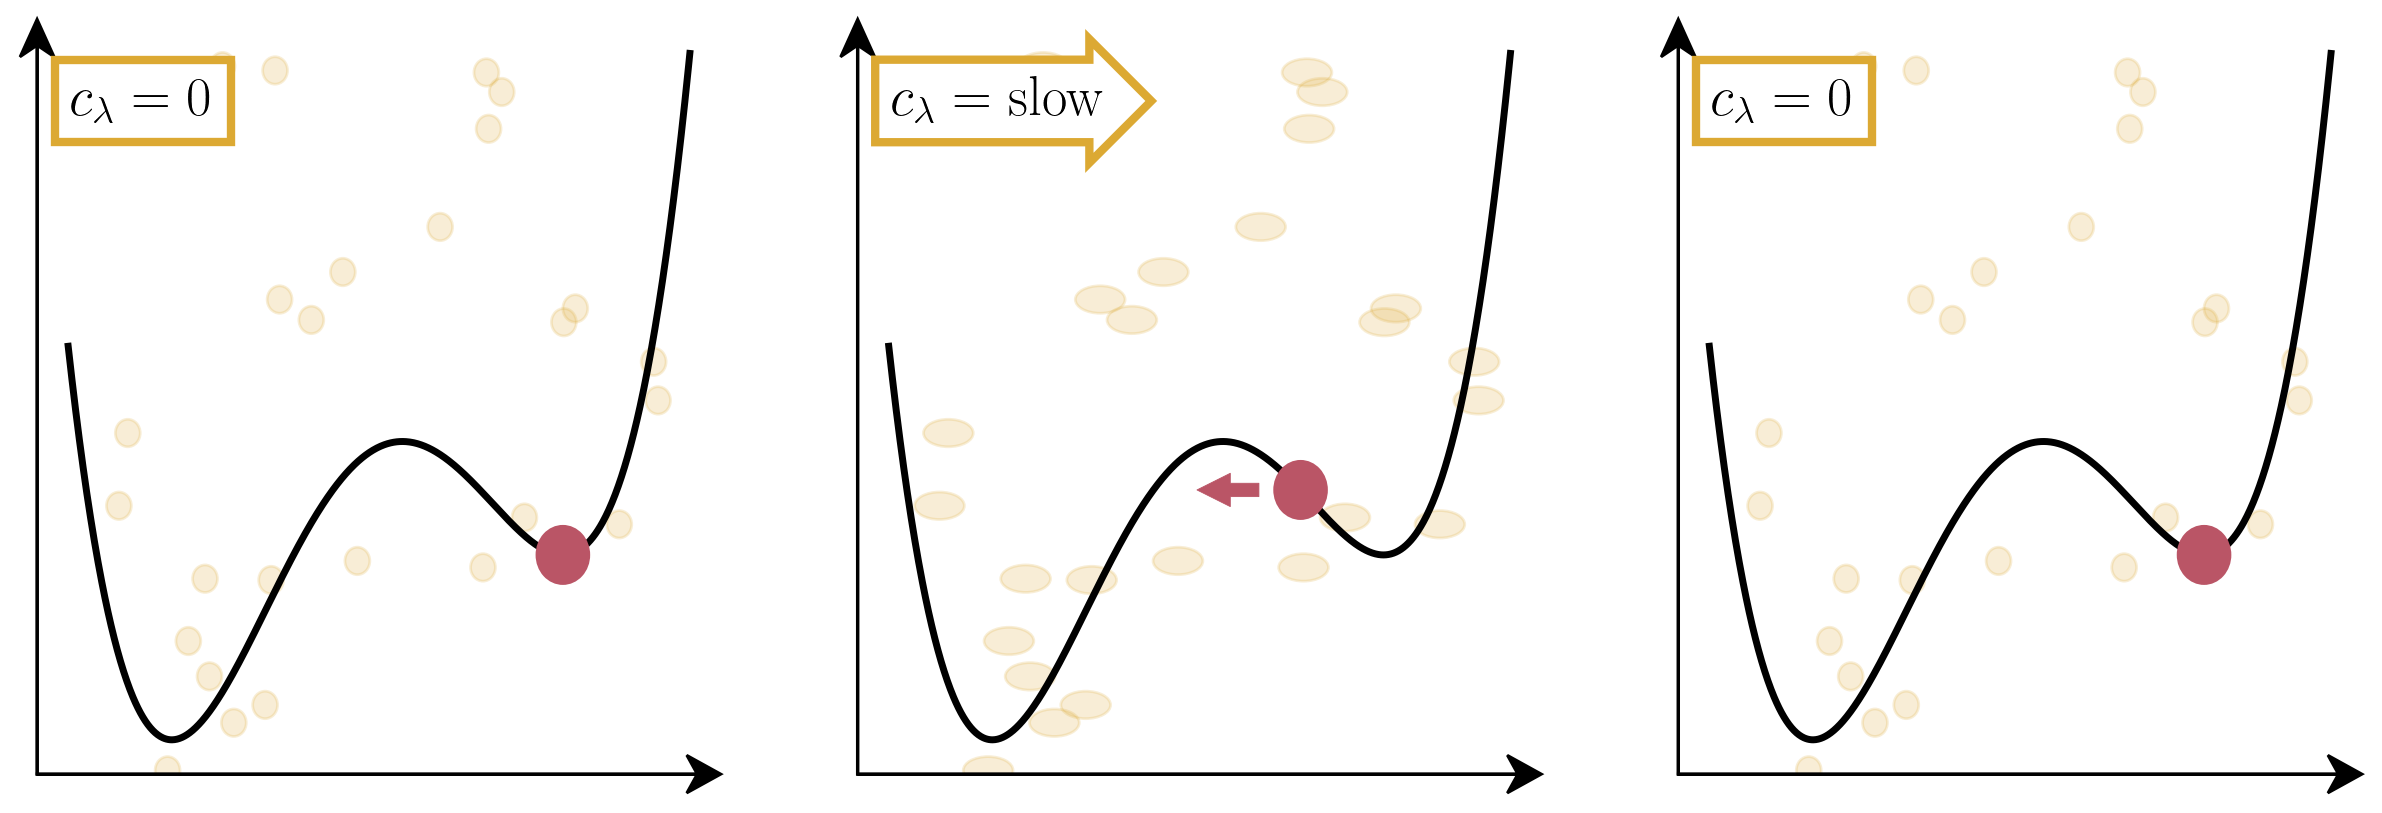
\includegraphics[width=\linewidth]{Images/Metrics/acceleration/slow}
	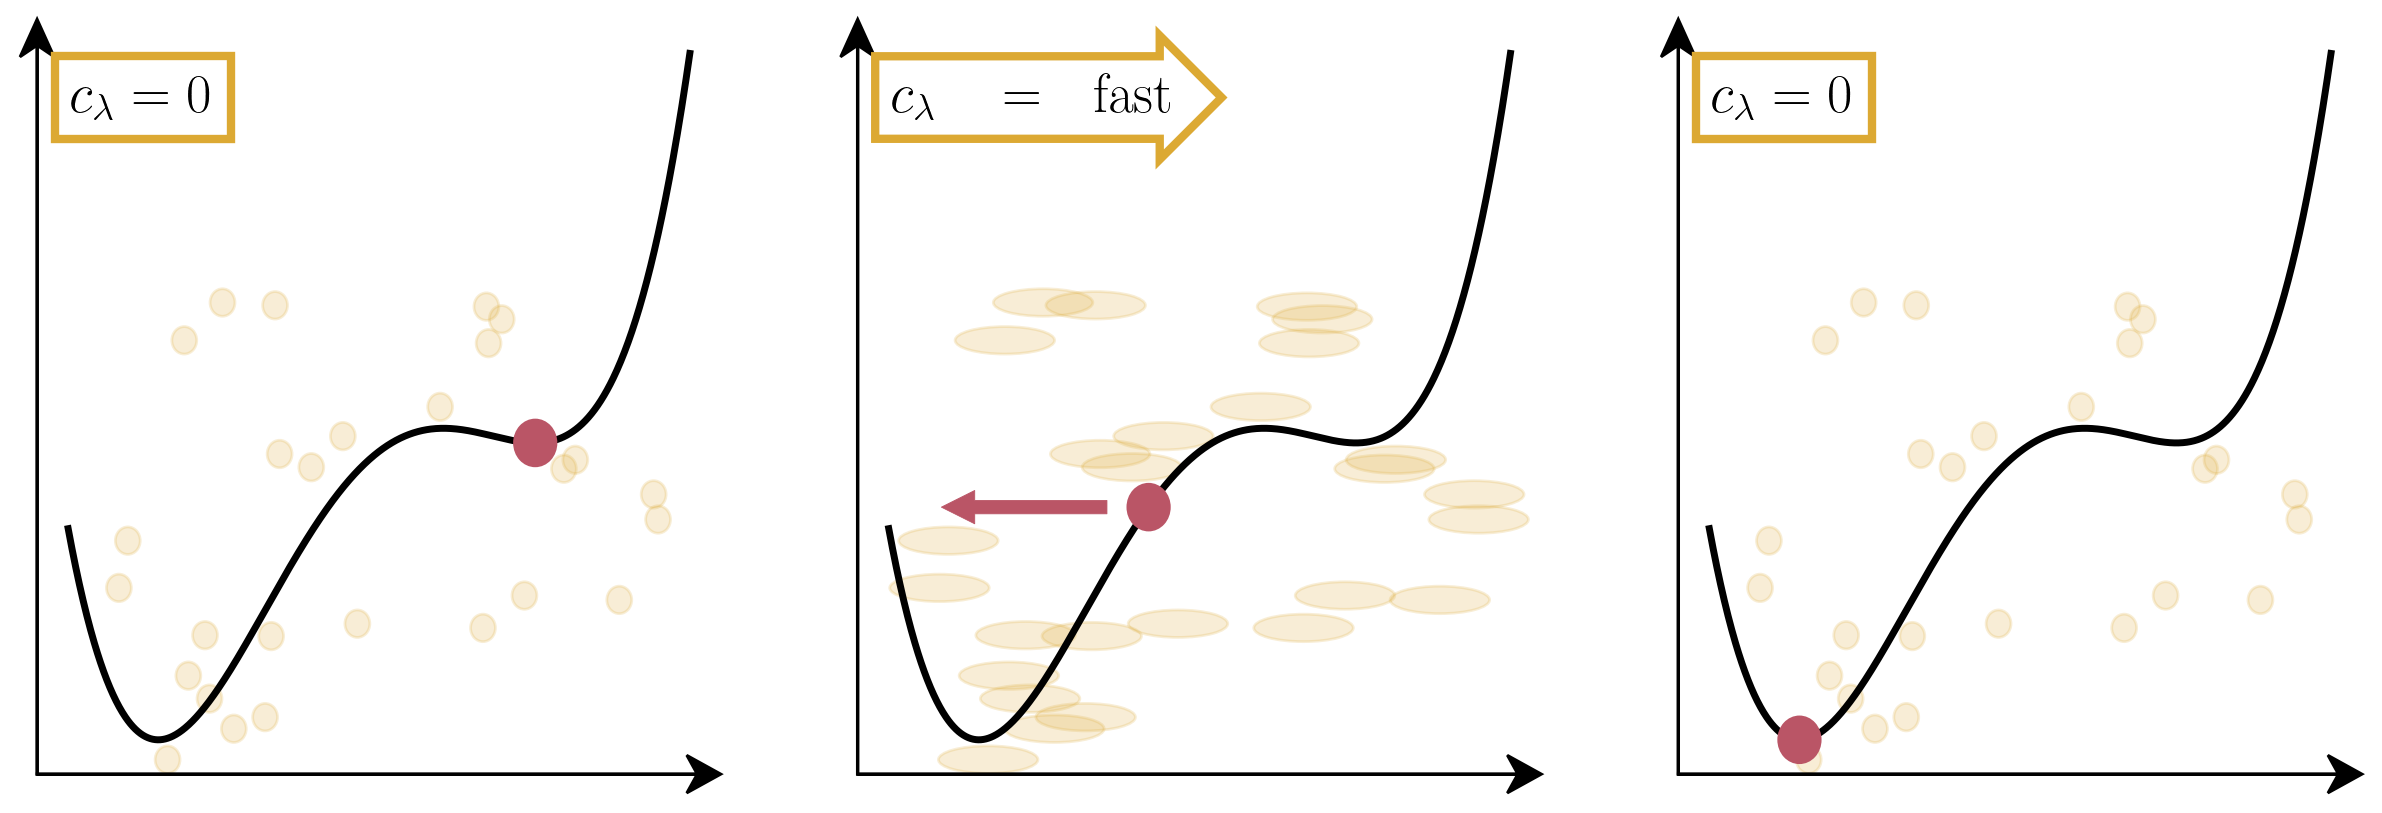
\includegraphics[width=\linewidth]{Images/Metrics/acceleration/fast}
	\caption{The effect of the sweeping parameter as the potential moves is like non-inertial force.  This scheme exemplifies a system that moves from one initial parameter to another, either slowly (top row) or fast (bottom row). In the fast case, the sweeping force tips the system (red) to the other equilibrium. The background yellow dots are there to show the movement of the surface.}
	\label{fig:slow}
\end{figure}

This idea gives an intuition on why \cref{eq:r_equilibrium} can still hold when $M(\la)$ as long as it stays close enough to the equilibrium.%, while for faster swipes the system will feel the slope of the rest of the surface. 


\subsection{Shock induced bifurcations, or S-tipping}

These are cases where an external shock, or an extreme event can kick the system out of its current basin of attraction \citep{Halekotte2020}.
\cite{Parry2022} discussed how, as the amazon forest loses resilience, a tipping might occur before   the global temperature (the control parameter), reaches the dynamical bifurcation and can be triggered by a  shock due to an extreme event, which in this case can be related to a large wildfire\footnote{This was proposed as a possible explanation by Peter Cox in a seminar \url{https://www.youtube.com/watch?v=kZqv3Tsew00&t=886s}}.  
The effect of shocks and extreme events as source of dynamical changes has been extensively studied as sources of tipping in financial markets   \citep{Sornette2009a}.



%cite jorrit paper on EWS
\section{Categories of EWS}

Most early warning signals  are based on the fact that, for most bifurcations, near the tipping point the system looses resilience and relaxation times become larger. 
This implies a growth of variance, and higher statistical fluctuations, correlation times\footnote{And therefore change in the noise power spectrum.} and correlation lengths. 


There are many reviews on EWS, like the ones by \cite{Scheffer2009, dakos2012_10.1371/journal.pone.0041010,Lucarini2014, Clements2018a,Feudel2018,Boettiger2013,Dutta2018,Bury2020}. 
Here we provide a short update summary of the kinds of EWS that have been proposed.
The EWS can be divided in four groups, depending in the method used, as follows:
\begin{enumerate}


\item{Metric Based}
The following EWS are based on  metrics related to  properties of the time series\footnote{This is a slight update from the review made by \cite{dakos2012_10.1371/journal.pone.0041010}}. 
\begin{itemize}
	\item Statistical quantities:  Variance or standard deviation (SD),  coefficient of variation ($SD/mean$), skewness, kurtosis, unbiased kurtosis estimators, relative tail weight.
	 These metrics measure a change in trend of the moments or percentiles of the distribution of an observable \citep{Xie2019,PhysRevE.100.013102,dakos2012_10.1371/journal.pone.0041010}.
	 These metrics can be performed either on raw data or de-trended data. 
	\item Spectral metrics: spectral density, spectral exponent, spectral ratio.
	These metrics measure a change in the spectrum of the noise. In some cases they can also predict the type of bifurcation and the frequency of limit cycles in Hopf bifurcations \citep{Bury2020}.
	\item Detrended fluctuation analysis indicator (DFA): It estimates a range of correlations by extracting the fluctuation of a time series of size $s$. If the time series is long-term power-law correlated, the fluctuation function $F(s)$ increases as a power law $F(s)\propto s^a$, where $a$ is the DFA coefficient, which is re-scaled to give the DFA indicator and tends towards $3/2$ close to the critical transition \citep{Peng1994,Livina2007}.
	\item Lag autocorrelations: Autocorrelation at lag-1 $\lag_1$, Auto-regressive coefficient of $\lag_1$, Return Rate (inverse of $\lag_1$, or 1-($\lag_1$)). Auto-correlation at other lags. \cite{Pavithran2021} also looks at the variance of the autocorrelation at some lag  as EWS.
	These metrics look at correlation in the temporal series to infer information on the stability of the system.
	\item Mixed metrics: Extended spatio-temporal correlation at lag-1 \citep{Tirabassi2022}, a mix of spatial and temporal lag-1 auto-correlation.
	There are two indexes proposed by \cite{Drake2010}: $W_1$ as the sum of the
	standardized differences of each statistic calculated in their work, and $W_2$ was
	calculated as the sum of the standardized deviations of each statistic from its long run average. 
	\item Conditional Heteroskedasticity \citep{Seekell2011}: It correlates the variance at different times.
	\item BDS test: Detects nonlinear serial dependence in time series. It fits the time series against linear models and test the null model on the residual noise to reject the i.i.d. hypothesis when near a critical transition \citep{Carpenter2011}.
	\item Mean fractal detrended fluctuation analysis (MF-DFA): This is a generalization of DFA for non-stationary time series, which analyses the critical slowing down though Husrts exponents. These exponents uncover multi-fractal properties of the time series data near transitions. 
	The Hurst exponent classifies the analyzed data between persistent ($0.5<H<1$), white noise ($H=0.5$) and anti-persitent $0<H<0.5$, with $H\rightarrow 0$ approaching the bifurcation and can be used also in chaotic systems \citep{Kaur2022,Bury2020,Pavithran2021}.
	
\end{itemize}


\item{Model Based}
EWS related to models or properties of nonlinear equations.

\begin{itemize}
	\item Non-parametric drift-diffusion-jump models (DDJ): It tries to fit parameters assuming an underlying drift-diffusion-model.
	\[
	dx_t=\mu(x_t,\dots,\la_t)dt+\sigma_D(x_t,\dots,\la_t)dW+d\left[ \sum_{n=1}^{N_t} Z_n\right] 
	\]
	where the coefficients are estimated by non-parametric regressions \citep{Ahn1988,Bandi2003,Carpenter2011a} and $Z$ refer to shock processes.
	\item Time-varying AR(p) models: 
	Here it is assumed that the systems evolves as 
	\begin{equation}
		x(t)=b_0(t-1)+\sum^{p_i=1}_i b_i(t-1)(x(t-i)-b_0(t-1))+\epsilon(t)\\
		b_i(t)=\sum^{p_i=1} b_i(t-1)+\phi_i(t)
	\end{equation}
where $b_0$ is related to the mean of the time series, and $b_i$ determines the dynamics around the mean.   $\epsilon$ is a random variable from $N(0,\sigma_\epsilon)$ and the equation for $b_i$ means it does a random walk dictated by the variances $\sigma_i$ from $\phi_i$.

	\item Threshold AR(p) models: This assumes a flickering between two states close to the transition, therefore it models the process like two AR(p) models switching at $x(t-1)=c$, where $c$ is a threshold to be defined, along with the parameters of the AR(p) models. 
	\item \cite{Laitinen2021} proposes other autoregressive models for evolving stochastic systems.
	\item Potential analysis: The idea behind this technique is reconstructing the local landscape of the associated potential assuming that 
	\begin{equation}
		dz=-\frac{dU}{dz}dt+\sigma dW
	\end{equation}
	where $dU/dz$ is a polynomial potential of even order, where the order of the best-fit polynomial reflects the number of potential stable states \citep{Livina2010,Livina2011}.

	\item Ising, networks and percolation models: These models use network and percolation results display the loss of resilience of a grid of points, or a network of agents. This is done the correlation or functional networks.
	Some network based precursors are the values of the degree (number of connections per node), assortativity (degree correlations), clustering, kurtosis rise, while the construction of functional networks through the Pearson correlation allows the study of percolation of the network as the system approaches the bifurcation,  through the study of the size of the largest connected component, the average cluster size, or the probability that a random node belongs to a component of a given size \citep{Rodriguez-Mendez2016a, Jager2017, Fullsack2022}.
	Furthermore, \citep{Dakos2017} propose the use of block decomposition methods, based on Kolomogorov complexity to identify transitions.
	Persistent homology and clustering have also been used to identify critical transition \citep{Mittal2017,Maletic2016} and is being applied  financial markets \citep{Gidea2020a,Ismail2022a}.
	\citep{Zhang2022} mean field network....
	
	As a practical example, use of network properties has also been used as EWS for sudden deterioration of diseases \citep{Chen2012a}, in particular as a warning for  diabetes-1 \citep{Liu2013}, and transitions in thermoacustic systems\footnote{\citep{Murugesan2016} compares several network properties as EWS. } \citep{Murugesan2016}.
	
	Many of the mentioned EWS are related to results of information theory, however we should also mention work where the entropy of the signals are directly used as EWS. In \cite{Chen2020} Shannon and Kolmogorov-Sinai entropy are used as EWS in chaotic systems, and compared to the Lyapunov exponent of the attractor. 
\end{itemize}
\item{Ordinal analysis}
%http://www.fisica.edu.uy/~cris/teaching/slides_masoller_uni.pdf
The symbolic approach
involves the transformation of a time series, $x(t)$, into a sequence of symbols, $s(t)$, by using an appropriated
codification rule. Complexity measures have been proposed to characterize the resulting symbolic sequence, a very popular one
being the permutation entropy (PE).
By measuring the entropy of the 'phrases' that results from the symbolic codification it is possible to characterize the different regimes and even predict regime changes
\citep{Masoller2015,Rubido2018,Boaretto2021}.

\item{Extreme Event Theory based}
EWS based on extreme value theory proposed by \cite{Lucarini2014}. Of which there are two equivalent approaches, one based on Generalized Extreme Value (GEV), and the Generalized Pareto Distribution (GPD). 

This metric is based on a change of convergence to the GEV (and GPD) of the block maxima distribution at the bifurcation. 
They have shown that, approaching the bifurcation, a system's GEV convergence with additive white noise goes to being linked to a GEV with positive shape parameter to negative going through zero at the bifurcation \citep{Faranda2014}. 


  

\item{AI based}

Lately there has been some developments on the use of deep learning algorithms trained on models with phase transitions that can be used as early warning tools \citep{Bury2021}.
In this model, the deep learning algorithm is trained on numerical simulations from an Ising model, where the system goes through several phase transitions of order $1$ and $2$. 
Since this phase transitions are linked to dynamical bifurcations,  the mechanisms for this are universal, this has been shown to predict bifurcations on test systems where is was not trained. 
This algorithms can be applied to spatial data obtained from satellite images, for example for arctic ice loss. 

Another recent development using Deep learning is the EWSnet network \citep{Deb2022}, a network trained on sets of different dynamical systems with a wide variety of bifurcations. 

\end{enumerate}


\subsection{EWS performance}

There are several things that can affect the performance of an early warning signal. Not only there are considerations inherent to the dynamical system, like the type of bifurcation, the source of noise, or the speed of the bifurcation parameter; but there are also data acquisition(sample frequency, sample spacing, available variables) and data treatment(type of detrending, length and type window either for detrending and for analysis) complexities to take into account. 

\begin{itemize}
	\item Time series performance
	\begin{itemize}
		\item Detrending 
		\begin{itemize} 
			\item Window size: In any detrending, the choice of window size affects the resulting detrended solution. De-trending on a small window can lead to keeping higher more fluctuations than wanted, too large a window (compared to the change on the bifurcation parameter) means keeping biases trends on the analyzed data. \citep{Jager2019}
			\item Window kernel: There are several types of detrending in the literature. From average moving window, to using a Gaussian kernel or  Lowess \citep{Dakos2008, Bury2020,Lenton2012} fit\footnote{Implementations of this detrending algorithms for Python can be found in the package ewstools: \url{https://github.com/ThomasMBury/ewstools}.}.  
		\end{itemize}
		\item Sample frequency: Sample frequency can affect EWS, specifically autocorrelation based signals, since they require interpolation to be estimated as a time series at constant intervals \citep{10.1086/681573}
		\item Noise: It has been shown that colored noise can have a negative impact on some EWS. In particular, signals  on additive or multiplicative noise, for the same underlying system, can display different behaviors  \citep{Kaur2022,Dutta2018,10.1086/681573}. 
		As shown by \cite{Boerlijst2013}, it is also relevant in which variable the noise is present. In this case, they show how EWS might be absent in the case of the absence of noise in the system's dominant eigenvalue for a saddle-nose bifurcation. And even then it there might not be EWS.
		An in depth  analysis on how the choice of observable and in which variable de noise is present is realized by \cite{Patterson2021}, where the effect of asymmetric noise is also explored.
		\item Analysis window: Some investigations on the importance of the lenght of the analysis window are done by \cite{Dutta2018}.
		\item Bifurcation parameter speed: a few work have been written where it is shown that the speed of the sweeping of the control parameter influences the quility and even the ability to have EWS as shown in \cite{Marcucci2019} and \cite{Kaur2022a}.		
	\end{itemize}
	
	For a larger review on performance of EWS, particularly for spatial EWS, we refer to \cite{Clements2018a,Feudel2018, Thompson2011}.
	
	\item Uncertainty estimation
	\subitem Different types of bootstrapping and it's efficiency and validity in the presence of data with heavy tails. For an example of EWS calculated using bootstrapping we refer to \cite{Bury2020}.
	
	\subitem Prediction reliability: Once a definition for a warning is made, the performance of the EWS can be tested by studying the ratios of false positives and false negatives by using an receiver operator characteristics (ROC) test as done by \citep{Boettiger2012a,Bury2020,Romano2018}.
	

\end{itemize}


\citep{Boettiger2012, Boettiger2013a}


Up to now we have mostly discussed in a sort of review manner, the developments on EWS that can be found in the literature. 


\section{The connection between extreme events and transitioning systems}

%This changes on the response of the system have implications on the behaviour of noise on the system, which translates to changes in the statistical properties of the distribution of the observables at this transitions.  


We now define several metrics to be applied to bifurcations in deterministic systems in the presence of noise, when external parameters are 'slowly' varying.
%Such metrics are specially useful when extreme events appear during the transit
%Indicators like the sample standard deviation, the autocorrelation, skewness and kurtosis, autocorrelation at lag-1 (AR-1) have been used as EWS\footnote{is it??, ask saulo a cite from paper using this in wave forecast}.

%\jk{A widely used index in that regard is kurtosis, i.e.,the 4th moment of the distribution }
The effect of CSD on the statistical properties of the system has inspired the proposal of a  so-called Pareto metric~\cite{Kasparian_pareto}.


\subsection{Tail related metrics}

The Pareto metric is one of many statistical functions that can be used to estimate  how 'heavy tailed' is a  probability distribution function (PDF). As discussed before, the CSD near the bifurcation of the system implies changes on the statistics of the noise.
In particular, this can give ride to  the appearance or frequency increase of extreme events in the systems close to tipping. 

In the rest of this section we will present a modification to the Pareto metric, and compare this to other tail related metrics used for EWS. We will first discuss this modification, and then construct a toy example of a sharp transition in sampled data, to understand how the metric behaves compared to others. 
Then we will use this metric on a series of systems with additive noise, by integrating  their stochastic differential equations (SDE), and discuss its performance. 

\subsubsection{Relative tail weight}

The Relative tail weight (RTW) metric considered in the present work is a slight generalization of the so-called Pareto metric proposed by \cite{Kasparian_pareto}. 
Given a time series of length $N$, this metric characterizes the weight of the PDF tail by calculating the total weight beyond a given threshold:
\begin{equation}
	M_p(I,k)=\frac{\sum^{k N}_{i=1} I_i}{\sum^{N}_{i=1} I_i}
	\label{eq:Pareto_original}
\end{equation}
%\begin{equation}
%   M(I,k)=\frac{\sum^{N}_{i=(1-k)N} I_i}{\sum^{N}_{i=1} I_i}
%  \label{eq:Pareto_original}
%\end{equation}
where the  individual measurements $I_i$ are sorted by descending order ($I_1\geq I_2\geq .. \geq I_n$) and $k$ defines the fraction of the data points that are attributed to the tail. 
For example, $k=0.2$ means that the metric considers the relative weight of the last $20\%$ of the distribution\footnote{This choice of $k$ was first inspired by the Pareto principle.}. 
This metric was successfully applied to the characterization of the pulse-to-pulse fluctuations of the spectral broadening in ultrashort laser filaments, showing that a long-tailed distribution only occurred on the edges of the self-phase modulation spectrum \citep{Kasparian_pareto}.

Since \cref{eq:Pareto_original} is a direct function of the measurement and not the distribution, whether the measurements take positive or negative values will change the result. 
% The original definition of equation \ref{eq:Pareto_original} depends on the absolute value of the mode, or the average of the probability distribution function (PDF).
Indeed, shifting the whole distribution to high values without deforming it will decrease the $M_p$ value since  measurements outside the $k$ percentile take negative values. 
We therefore adapt a new definition by shifting the distribution so that the minimum data point $I_N$ is set to 0. Therefore,

\begin{equation}
	\mathrm{RTW}_{max}(I,k)=\frac{\sum^{k N}_{i=N} (I_i-I_N)}{\sum^{N}_{i=1} (I_i-I_N)}=\frac{\sum^{k N}_{i=N} I_i-k N I_N}{\sum^{N}_{i=1} I_i-NI_N} 
	\label{eq:pareto_offset}
\end{equation}


%  \begin{equation}
	%     M(I,k)_N=\frac{\sum^{N}_{i=(1-k)N} (I_i-I_0)}{\sum^{N}_{i=1} (I_i-I_0)}=\frac{\sum^{N}_{i=(1-k)N} I_i-k N I_0}{\sum^{N}_{i=1} I_i-NI_0} 
	%    \label{eq:pareto_offset}
	%\end{equation}
	
	\begin{figure}[h]
		\centering
		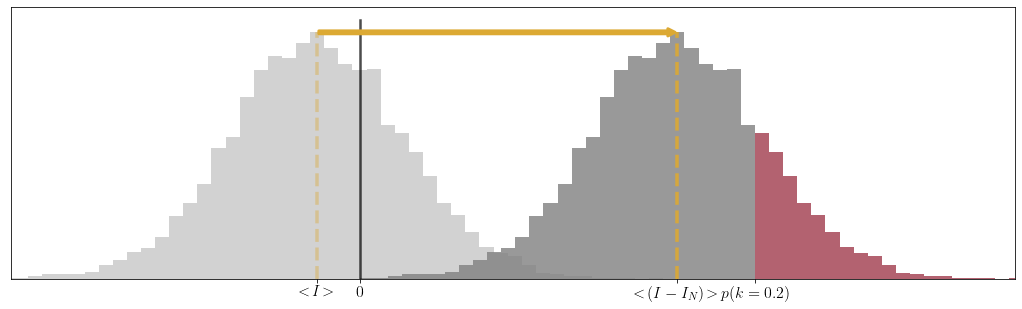
\includegraphics[width=\columnwidth]{Images/Metrics/pareto_shift_explanation.png}
		\caption{Shifting the distribution to have it defined positive, and taking integrating over the highest $k$ percentile (magenta).}
		%	\caption{Events per ms}
		\label{fig:pareto_shift}
	\end{figure}
	
	This adapted $M$ is quite dependent on the value of $I_N$, so that it is mostly adapted to asymmetric distributions where the low-value side cutoff is quite abrupt, so that for $N$ sufficiently large, $I_{min}$ of each data set should converge. 
	
	
	\subsubsection{Extension to consider heavy-tailed distributions on the left side of the PDF}
	
	As discussed above, the definition of $M_p$ in \cref{eq:pareto_offset} focuses on heavy tails on the right side of the PDF (large values). To extend it, we propose to flip the distribution as a whole around its median, then apply the definition in \cref{eq:pareto_offset}. The choice of the median as the flipping axis is consistent with the fact that the Pareto-metric focuses on percentiles. Thus, we consider the flipped intensity distributions:
	
	\begin{equation}
		 \hat{I}_i=2I_{50}-I_i 
	\end{equation}
	and the metric for low values becomes $\mathrm{RTW}_\textrm{low}(I,k)=\mathrm{RTW}_\textrm{max}(\hat{I},k)$
	
	In this way the metric  provides information on the heaviest tail on either side:
	
	\begin{equation}
		\begin{aligned}
		 \mathrm{RTW}(I,k)&=\max(\mathrm{RTW}_\textrm{low}(I,k),\mathrm{RTW}_\textrm{max}(I,k))\\
		 &=\max(\mathrm{RTW}_\textrm{max}(I,k), \mathrm{RTW}_\textrm{max}(\hat{I},k))
		\end{aligned}
	\end{equation}
	
	Here the choice of the $maximum$ of either RTW$_\textrm{max,low}$ is because we want to know what is happening to the more 'extreme' tail, whichever it might be. 
	
	
	Another possible choice is to construct a complex metric RTWc defined as
	
	\begin{equation}
		\mathrm{RTWc}(I,k)=\mathrm{RTW}_\textrm{max}(I,k) + i\, \mathrm{RTW}_\textrm{low}(I,k)
		\label{eq:RTWc}
	\end{equation}
	
	In this case, the absolute value gives information of the intensity of the tail weight in the distribution taking into account both tails, while the angle between $\textrm{RTW}_\textrm{max}$ and $i \textrm{RTW}_\textrm{low} $ encodes information of the asymmetry between the tails.
	
	In this case, for a symmetric distribution the complex metric is related to the one defined by the maximum as 
	
		\begin{equation}
	|\mathrm{RTWc}(I,k)|=\sqrt{\mathrm{RTW}_\textrm{max}^2+\mathrm{RTW}_\textrm{low}^2}=\sqrt{2}\,\mathrm{RTW}_\textrm{max}=\sqrt{2}\,\mathrm{RTW}
		\end{equation}
	
	Thus, the absolute value of RTW is no longer bounded between $(0,1)$ but between $(0,\sqrt{2}$).
	
	
	\subsubsection{Kurtosis and unbiased estimators}
	
	
	The kurtosis of a distribution evaluates the flatness of the PDF mode and the extension of the tails. It is defined as
	\begin{equation}
		\beta_2 = \frac{\sum_{i=1}^N{\left(I_i - <\!I\!>\right)^4}}{\sigma^4}
	\end{equation}
	where $\sigma$ is the standard deviation. While kurtosis is good as a measure of the tails \citep{kurtosisRIP}, some properties like its bias (see below) and heavy dependence on single and large events \citep{KIM200456} mean it might not be the best choice under some circumstances. 
	
	In this work we use the excess kurtosis $\tilde{\beta_2}=\beta_2-3$, defined this way to keep the Gaussian excess kurtosis equal to $0$.
	
	We will show that the use of excess kurtosis for some applications as an indicator for the tail is not practical, and it might be better to use another indicator for real, finite amounts of data. 
	In \cite{Bono_2019,KIM200456} it is recalled that kurtosis can be a biased statistic and two unbiased kurtosis estimators, the Hogg $Hg$ and the Moors $Mo$, are explored:
	
	\begin{equation}        	   
		Hg=\frac{U_{0.05}-L_{0.05}}{U_{0.5}-L_{0.5}}-2.59
		\label{eq: Hogg}
	\end{equation}
	
	\begin{equation}               
		Mo=\frac{(E_7-E_5)+(E_3-E_1)}{E_6-E_2}-1.23
		\label{eq: Moors}
	\end{equation}
	
	where $U_{m}$ and $L_{m}$ refer to the mean of the Upper and Lower $m$ quantiles, respectively. This means that $U_{m}=\frac{1}{m}\int_{1-m}^1 F^{-1}(y)dy$ and $L_{m}=\frac{1}{m}\int_{0}^m F^{-1}(y)dy$, where $F$ is the cumulative distribution function for ${I_i}$\footnote{\cite{Bono_2019,KIM200456} have  different definitions of the unbiased kurtosis estimators $Kr_2$ and $Kr_3$. \cite{Bono_2019} uses these definitions for the Hogg estimators with $m=0.05$ (\cref{eq: Hogg}) and $m=0.2$ (\cref{eq: Hogg}). While \cite{KIM200456} defines $Kr_2$ as the Moors estimator (\cref{eq: Moors}) and $Kr_3$ as the Hogg estimators with $m=0.05$ (\cref{eq: Hogg}). }.
	 $E_n$ in \cref{eq: Moors} are the respective $n$-th octiles. 
	Both definitions are displaced with respect to their values for a Gaussian distribution to be compared to excess kurtosis.
	
	It should be noted that in \cite{KIM200456} another tail metric by Crow and Siddiqui (page 6) is also explored:
	
	\[
	Kr_{CS}=\frac{F^{-1}(1-\alpha)+F^{-1}(\alpha)}{F^{-1}(1-\beta)-F^{-1}(\beta)}
	\]
	
	with $\alpha = 0.025$ and $\beta= 0.25$. 
	However is it shown that this is not as good compared to $Hg$ and $Mo$, and thus will not be considered in this work.
		
	\subsection{Common values}
	
	These metrics share a basic property. They take constant values for some distributions of given shape, like the uniform distribution, the Gaussian distribution, the Rayleigh distribution and the exponential distribution (Table \ref{table: constant shape}).
	
	\begin{table}[h]
		\centering
		\caption{ \label{tab:indicescte} Metric values for typical distributions.}
		\begin{tabular}{| l | l | l | l  |l | l |}
			\hline
			Distribution & RTW & $\left| \mathrm{RTWc}\right| $  & Excess kurtosis  & Hg & Mo\\
			\hline
			Uniform & 0.36 & 0.5 & -1.2  & -0.69 & -0.24 \\
			Gaussian& 0.27 & 0.38 & 0 & 0 & 0\\
			Rayleigh & 0.36 & 0.44 & 0.24 & -0.11 & -0.03\\
			Exponential & 0.52 & 0.57 & 6 & 0.28 & 0.56 \\
			\hline
		\end{tabular}
		\label{table: constant shape}
	\end{table}
	
	This means that, no matter which scale parameter is used for these distributions, they have a constant value for all such tail metrics. 
	Thus, we consider to be requirement of any tail metric. \footnote{Maybe a measure of sensitivity for a given statistic $St$ could be $\frac{Abs(St(gaussian)-St(exponential))}{St(gaussian)}$.. though maybe it is better between two values of the same distribution.. like gamma(0.5) and gamma(2).. so this is a slope in a plot St(gamma) vs. gamma. It would be more apples-to-apples comparison. Finding a distribution that changes linearly for some metric would be best(?)
	}
	
	This is not true for distributions like the Weibull, the Gamma or the Lognormal (among others) that change shape as a function of their parameters\footnote{The excess kurtosis of the lognormal is $K=e^{4\sigma^2}+2e^{3\sigma^2}+3e^{2\sigma^2}$-6; for the Gamma function $K=6/\alpha$ .}.
	
	For comparison with \cite{Bono_2019}, we add the table \ref{table: changing shape}.
	
	\begin{table}[h]
		\centering
		\begin{tabular}{| l | l | l | l | l | l |}
			\hline
			Distribution & RTW & $\left| \mathrm{RTWc}\right| $  & Excess kurtosis\footnote{Excess kurtosis for Gamma PDF is $6/\alpha$; for lognormal distribution is $e^{4\sigma^2}+2e^{3\sigma^2}+3e^{2\sigma^2}-6$} & Hg & Mo\\
			\hline
			lognormal($\zeta=1$,$\alpha=0.5$) & 0.39 & 0.44 & 5.9  & 0.28 & 0.06 \\
			Gamma ($\alpha=0.5$)& 0.65 & 0.68 & 12  & 0.68 & 0.25 \\
			Gamma ($\alpha=2$)& 0.43 &0.48 & 3 &  0.12 & 0.03 \\
			Gamma ($\alpha=4$)& 0.36 & 0.43 & 1.5 & 0.06 & 0.21\\
			\hline
		\end{tabular}
			\caption{ Some values for shape dependent distributions. Here $\alpha$ is the shape parameters of the distributions.\label{tab:indices}}
		\label{table: changing shape}
	\end{table}
	
%\url{https://variation.com/wp-content/distribution_analyzer_help/hs128.htm}}
	
	
	
	
	
	%	\begin{center}
		%		\underline{Table of distributions with constant value: \ag{Make this a real table, with a proper legend + label}}
		%		
		%		\begin{minipage}[t]{0.32\textwidth}
			%			Pareto centered $k=0.2$
			%			
			%			\begin{tabular}{ l | c }
				%				\hline			
				%				Uniform & 0.36 \\
				%				Gaussian & 0.266 \\
				%				Rayleigh & 0.36 \\
				%				Exponential &  0.52 \\
				%				\hline  
				%			\end{tabular}
			%		\end{minipage}
		%		\begin{minipage}[t]{0.32\textwidth}
			%			Excess Kurtosis
			%			
			%			\begin{tabular}{ l | c }
				%				\hline			
				%				Uniform & -1.2 \\
				%				Gaussian & 0. \\
				%				Rayleigh & 0.252 \\
				%				Exponential & 6  \\
				%				\hline  
				%			\end{tabular}
			%		\end{minipage}
		%		\begin{minipage}[t]{0.32\textwidth}
			%			Rogue event indices \ag{What are the two columns?}
			%			
			%			\begin{tabular}{ l | c | c }
				%				\hline			
				%				Uniform & 0. &  0  \\
				%				Gaussian & 0. &  0 \\
				%				Rayleigh & 1 &  1/45= 0.02 \\
				%				Exponential &  45 &  1\\
				%				\hline  
				%			\end{tabular}
			%		\end{minipage}
		%		
		%	\end{center}
	
	\subsection{Convergence}
	\label{sec:EWS_convergence}
	For real applications, it is important to compare how quick these metrics stabilize to a given value under the same circumstances. 
	It is clear that, since they measure the tails, a lot of points are needed for these metrics to be reliable. 
	The need for big datasets for the kurtosis in the presence of outliers is  discussed in depth in~\cite{KIM200456}, together with a comparison to $Hg$ and  $Mo$. Here. we  also discuss the  RTW. 
	
	To visualize this, we consider a big sample ($10^5$) for a given distribution, in this case the Gamma distribution with $\sigma=2$, and we see how the value of each statistic changes taking larger and larger sub-samples by steps of 200 points. 
	
	This shows how the values of the metrics  change for a given realization as the we consider a larger and larger sample size. 
	By doing the same plot after shuffling the data of the original realization, we can estimate the dispersion due to the different paths  the same sample can take,  until they converge to the value of the original realization. 
	
	
	
	\begin{figure}[htb]
		\centering
		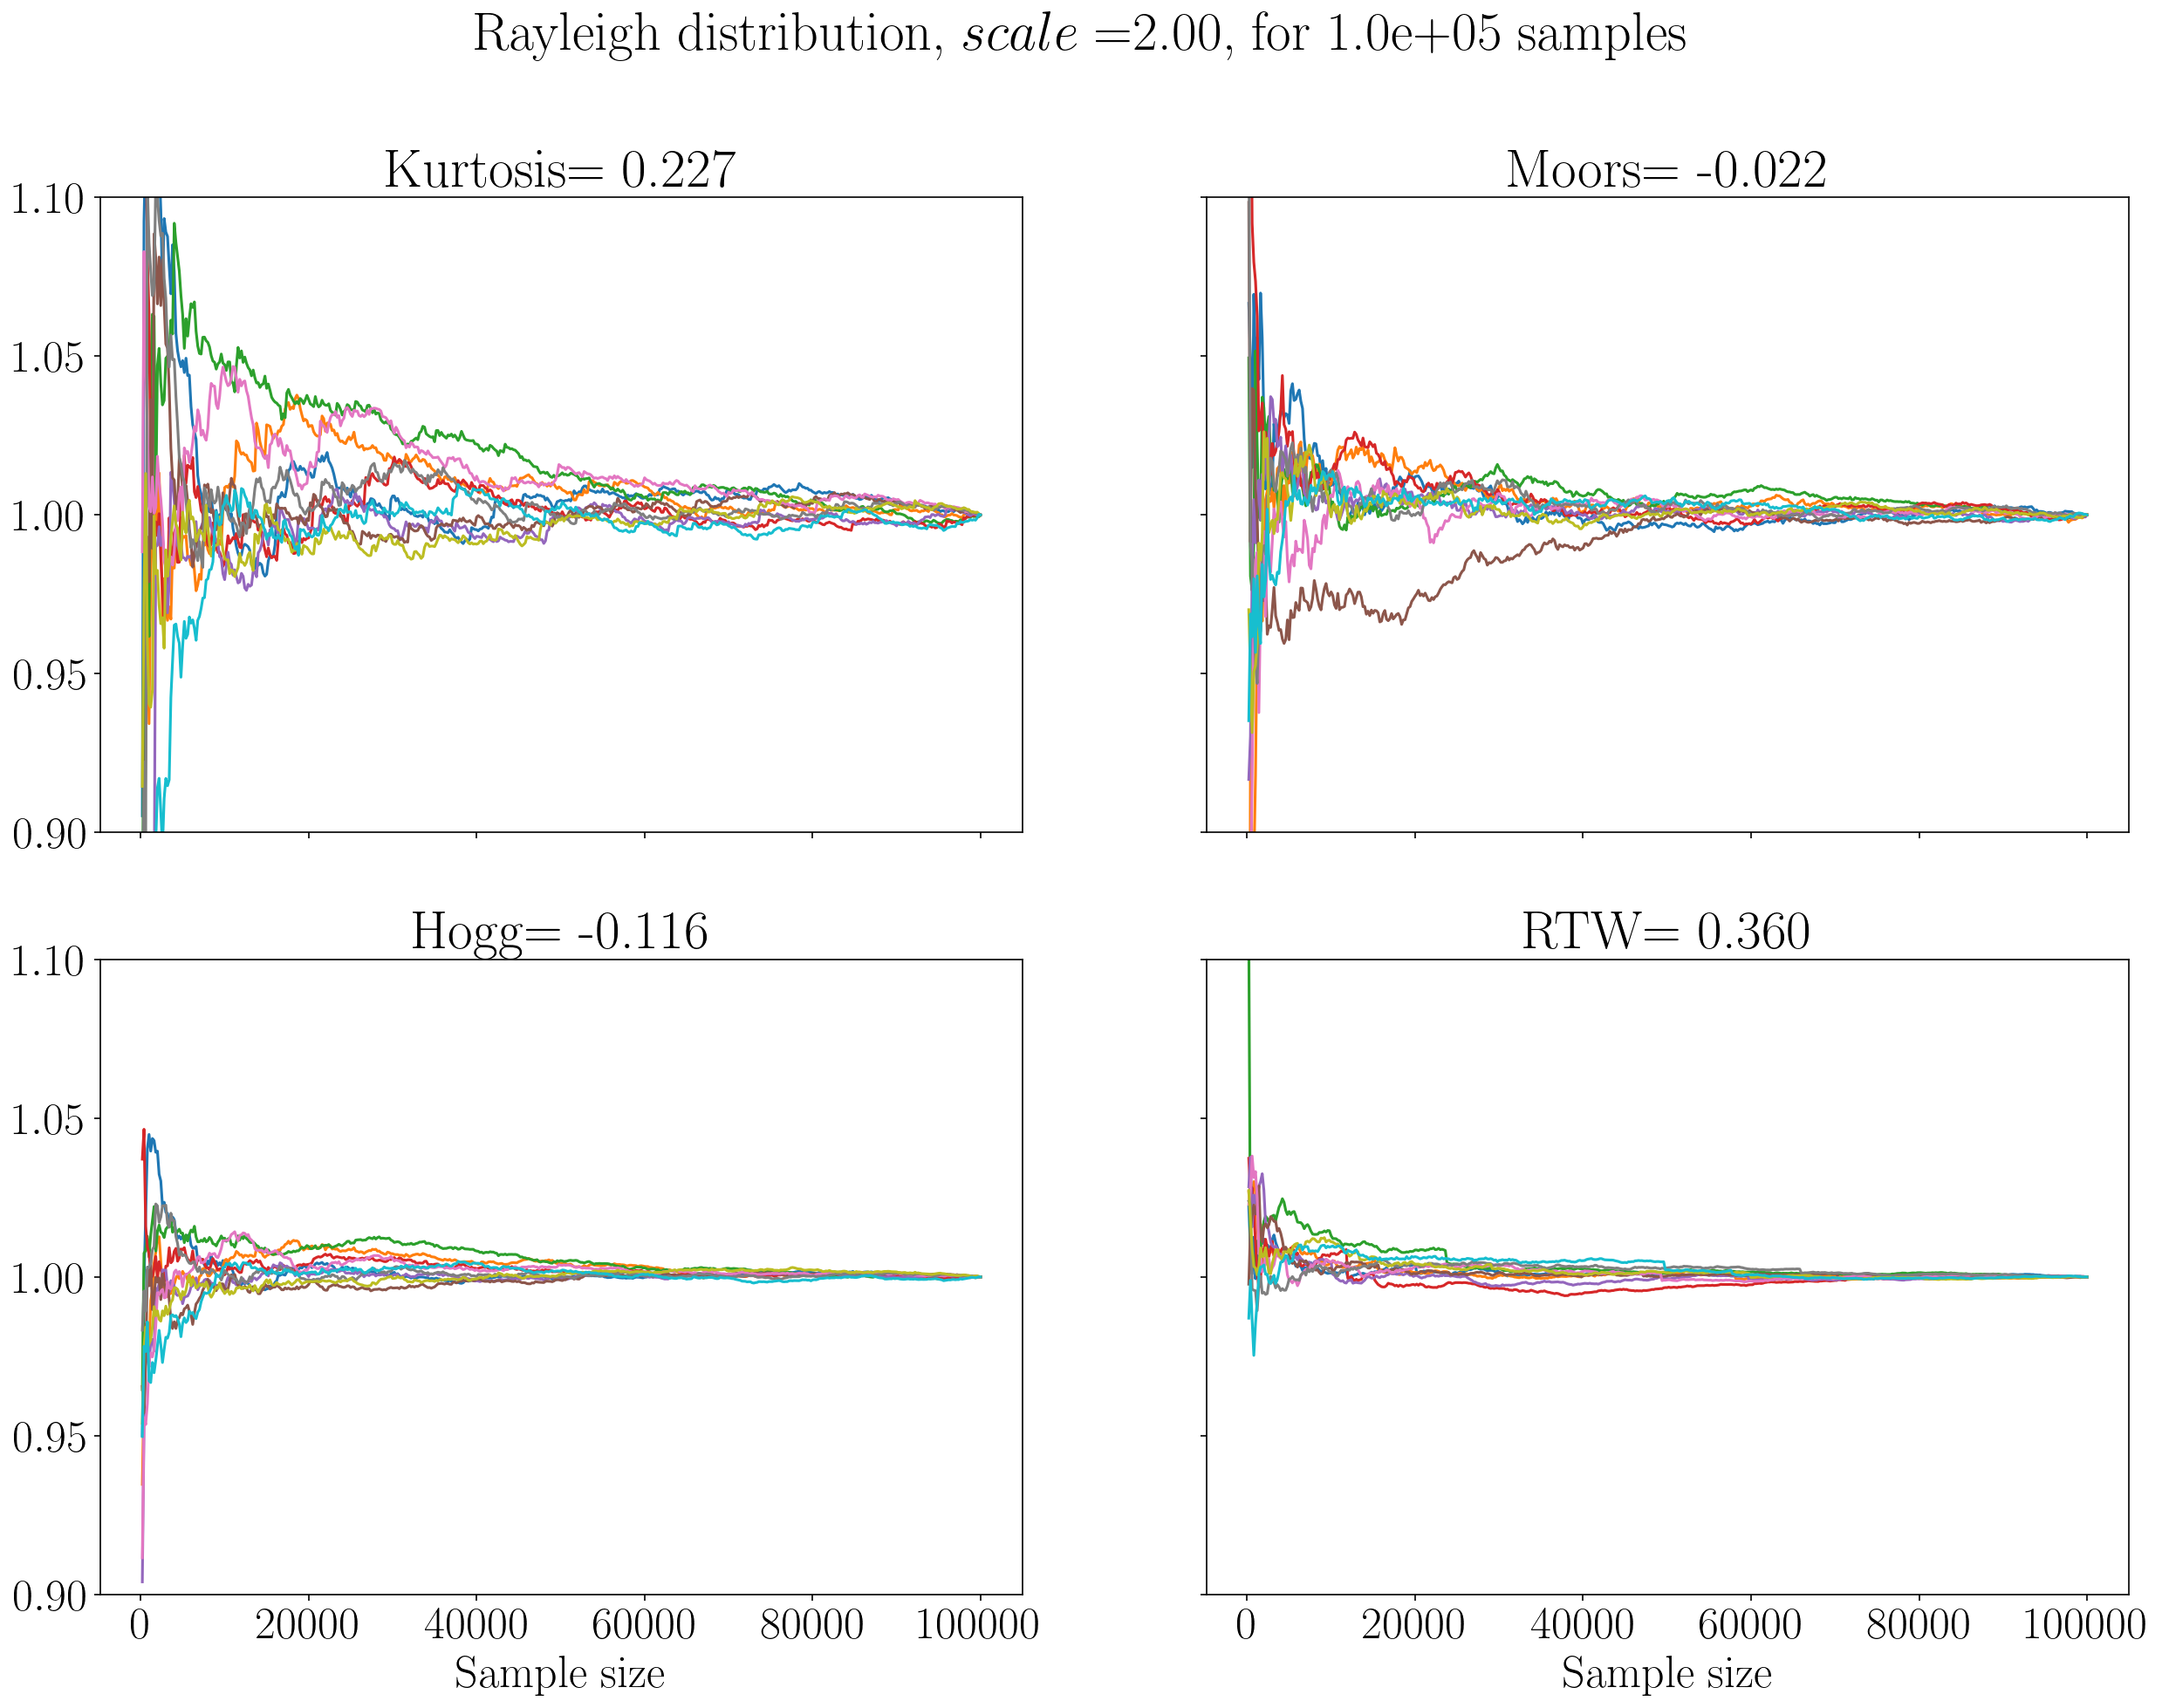
\includegraphics[width=\linewidth]{Images/Metrics/boot_rayleigh_convergence.png}
		\caption{ Evolution of the tail statistics: Kurtosis, Moors, Hogg and RTW calculated for a Rayleigh distribution of sample size $10^5$. 
		Each statistic is calculated every $200$ samples. After this is over for all the sample length, the original sample is scrambled and the same procedure is done. This is to show how fast this statistics converge and how much they might fluctuate due to an update of the sample. 
		Each statistic is calculated without correcting for the Gaussian value (ie. is calculated on  the kurtosis, not the excess kurtosis, etc.. ) and normalized to the final value. Only the title values are calculated corrected for the Gaussian values as defined above.	
		}
		\label{fig:convergence_1}
	\end{figure}
	
	Figure \ref{fig:convergence_1} shows this evolution for the excess kurtosis,the $Mo$, the $Hg$ and RTW metrics.
	This is done by taking an initial sample of a Rayleigh distribution of size $10^5$. 
	Each statistic is calculated every 200 samples, i.e for sample sizes $\left\lbrace 200, 400, 600, \dots, 10000\right\rbrace$, then the original sample is shuffled and the same procedure is done, and the shuffle is repeated 10 times.
	This means that, for each statistic, each shuffle converges to the same value since the final distribution is based on the same $10^5$ data points.  
	These statistics are calculated for their definitions without correcting to the Gaussian value and then normalized to the final value. 
	The values for the titles are calculated for the  $10^5$ data set on the excess definitions (corrected to the Gaussian values.)
	
	This displays of the robustness of these metrics, since we can see that the kurtosis is more affected by the update on the data, and even when sampled from the same parent distribution after 7000 (70\%) points, it still has fluctuations of about 2\%, while the other statistics show a better performance much earlier.	
	
	
	\subsection{Bootstrapping}
	\label{sec:EWS_boots}
	Given the sensible nature of metrics related to tail statistics, especially the kurtosis, 
	it is important to try to achieve a reliable result with the finite data-set we handle and, if possible, to give an estimate of the error when calculating such values. 
	
	For this purpose, we use a simple non-parametric bootstrapping method to calculate mean values and expected errors for the metrics, following  \cite{Wright2011}. 
	
	If $\Bar{x}$ is the data to be analyzed:
	\[
	\Bar{x}_0={x_0,x_1,\dots,x_n}
	\]
	the bootstrapping method consists of making new sample sets by randomly shuffling the data ${x_j}$ in the original sample, and applying the analysis to these new $\Bar{x}_k$ samples:
	
	\[
	\Bar{x}_k={x_{k_1},x_{k_2},\dots,x_{k_n}}
	\]
	
	Then, the average of the resulting analysis in all the samples, for a sufficiently large set of re-samples, converges to the real statistic. 
	In this way, we can get better confidence on our results, without taking new measurements.
	
	Since the resulting distribution of all the samples should converge to a normal distribution, this also gives us an estimate of the error of our result. 
	\footnote{In \cite{Wright2011} it is briefly mentioned that this does not always work well for kurtosis, but there is no a better method cited. Since kurtosis is really sensitive to outliers, the bootstrapping will oscillate  and an arbitrarily large set of re-samples might need to be made to have a clean normal distribution (this could be tested by fitting and the $\chi^2$?)}

	
	%\href{http://dx.doi.org/10.2139/ssrn.3360903 }{\underline{this paper} Davide talks about saddle point approximations and edgeworth series like better options } }}

\begin{figure}[H]
\centering
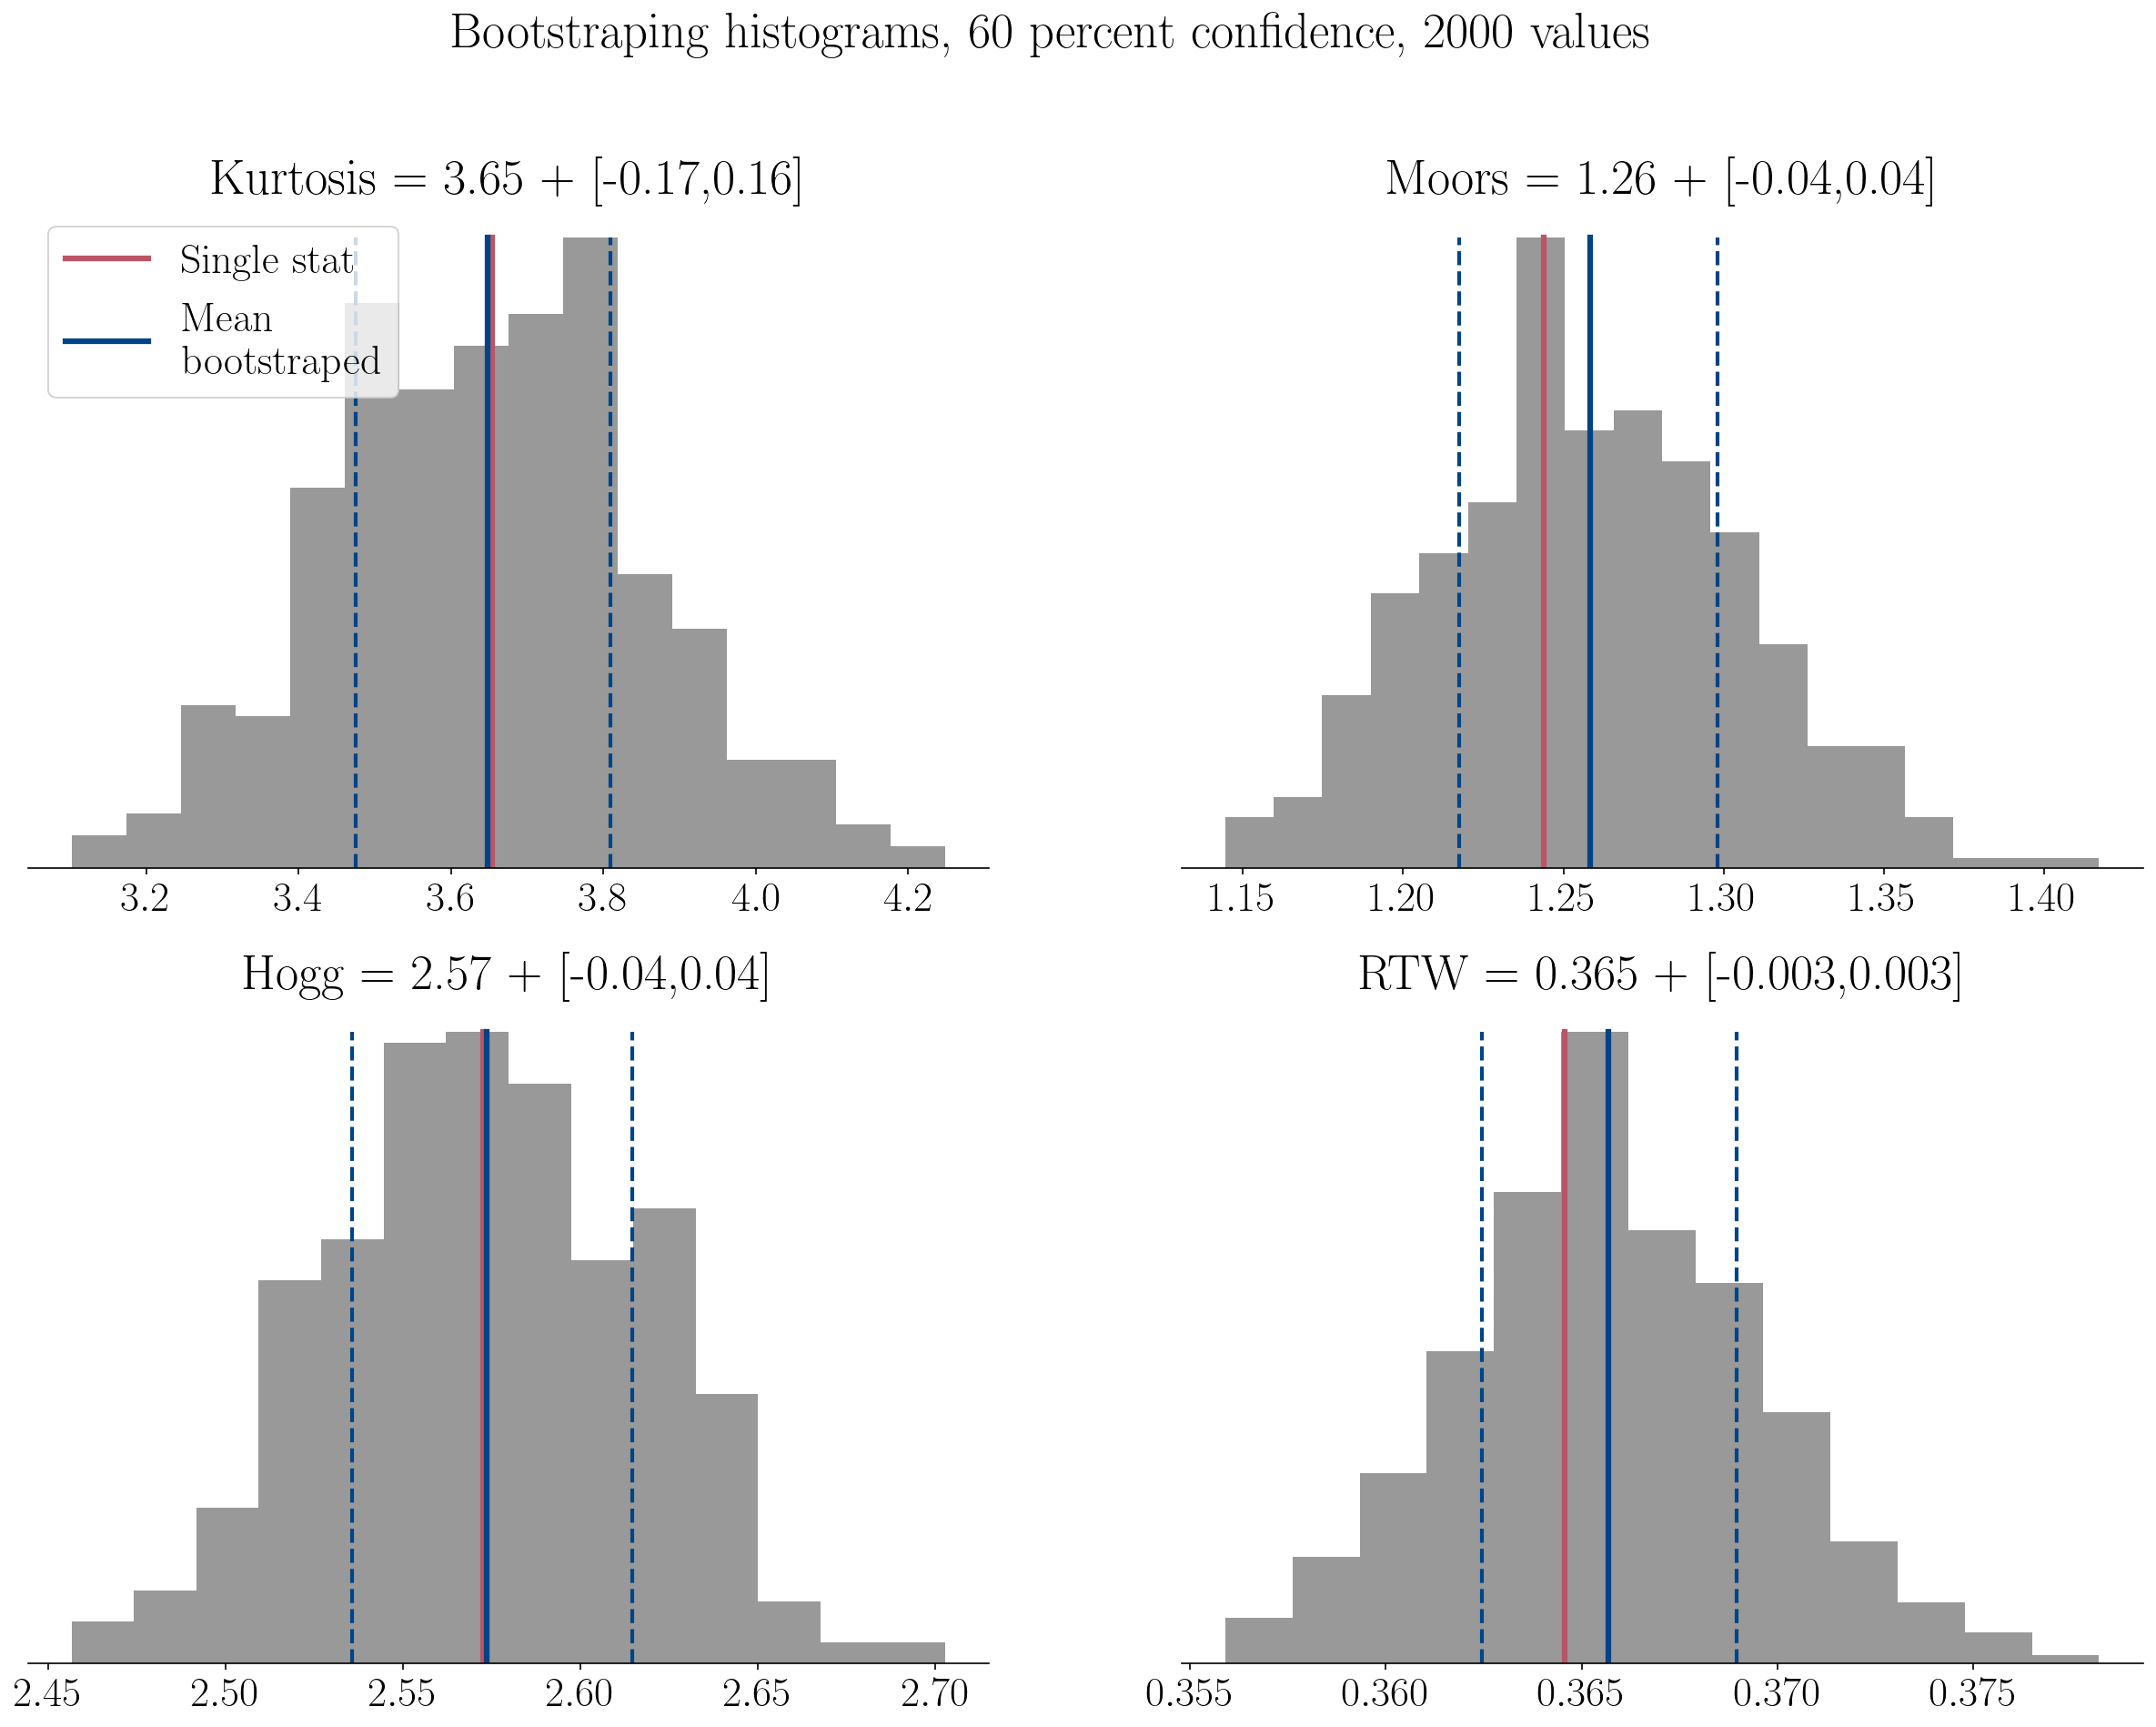
\includegraphics[width=\columnwidth]{Images/Metrics/boot_histograms_rayleigh_2000_400.png}
\caption{ Bootstrapping examples applied to a Rayleigh distribution with 2000 samples, after 400 resamples. The red line indicates the statistic calculated from bootstrapping, while the blue line is calculated from the samples, dashed blue indicate the 0.2 and 0.8 percentiles.  }
%	\caption{Events per ms}
\label{fig:Boots_example}
\end{figure}

In figure \ref{fig:Boots_example}  the result of applying the simple bootstrapping method to a sample of 2000 points from the Rayleigh distribution for 400 resamples is shown.
Each bootstrapping is done by resampling a data set of 70\% of the original data.
Applying this procedure for the Kurtosis,  $Hg$,  $Mo$ and  RTW yields Kurtosis$=3.65\pm 0.17$; $Hg=2.57\pm 0.04$, $Mo=1.26\pm 0.04$ and RTW=$0.365\pm 0.003$, where the errors are taken to have a $60\%$ confidence (0.2 and 0.8 percentiles) and the statistics are not corrected to the Gaussian values to better exemplify the relative error.

These results also show how more robust the RTW metrics are, since the relative errors after this particular bootstrapping are much lower than the relative error of the estimators and much lower than the relative error of the kurtosis.    

Appendix \ref{apx:boots} shows the same analysis for an exponential distribution to show the redundancy of the results.



%  \subsection{Transitions}




\section{Stochastic differential equations (SDE)}

A proper testbed for EWS is to  simulate what happens in a dynamical system when noise is part of the dynamic and a control parameter changes continuously,  and see if we can predict its transition.

Since real systems (and measurements) have noise, this is particularly relevant in systems where the noise can  affect the dynamics of the system \citep{Coulson2004}.

Such systems meed to  be described by some differential equation that has the noise incorporated in the integration scheme, i.e. stochastic differential equations (SDE). Though technically speaking the differential equation is no longer continuous since there are stochastic perturbations at each integration step, and therefore there is a fractality to the way the noise exists in these equations, there are  many cases in which these equations can be solved in a probabilistic sense. 


This means that each integration now is just a path of the many possible paths the system can take in its evolution, each one with some probability. 


%\subsection{Simulations on stochastic differential equations}

We consider a deterministic nonlinear differential equation $\dot{\vec x}=f(\vec x,\vec \lambda)$, which in this context will be called \textit{deterministic backbone}, where $\vec x$ is a variable of the system and, for our purposes the observable, and $\vec \lambda$ is a set of parameters of the system.

In general, we can consider a system which can not only have some constant internal noise but also be perturbed by 'kicks'.
Such a system can be simulated as a drift-diffusion-jump model: 
\begin{equation}
	\mathop{d\vec x}=f(\vec x,\vec \lambda)\mathop{dt}+g(\vec x,\lambda)\mathop{dW}+c\mathop{dJ}
	\label{eq: SDE general}
\end{equation}

In this case $f(\vec x,\vec \lambda)$ is the deterministic backbone of the equation, $g(\bar x,\bar \lambda)$ is the noise intensity which can include interaction between the data and the noise, $\mathop{dW}$ is a Gaussian (white noise) process (Wiener process) with zero mean and unit variance ($N(0,1$)) and $\mathop{dJ}$ is a Poisson process with positive intensity $c$. 
If the function $g(x,\lambda)=\sigma$, then the system has additive noise; if $g(x,\lambda)=\sigma x$, the process has multiplicative noise.

In equation \eqref{eq: SDE general}, the Wiener process implies a constant white noise, while the Poisson process models occasional perturbations in the system, usually called 'jumps' or 'kicks' \citep{bibid}.

This means that besides the freedom we have when selecting the speed at which the parameter changes ($\la=\la(t)$), we also have freedom on the choice in the noise intensity, and the process from which it comes from, which influences the color of the noise \citep{Kaur2022}. 

Each of this options greatly complexifies our analysis. Even when considering only Wiener processes, there are fundamental differences between additive and multiplicative noise \citep{Alberti2021} since multiplicative noise effectively can change the dimensionality of attractors and  the stable manifolds in a different way from additive noise. 
Even only considering additive noise, having some correlation on the noise can change bifurcation points and early warning performance as shown by \cite{Kaur2022}.


For the sake of simplicity, in this work we will focus on  one dimensional systems with additive white noise. 



\subsection{Ornstein-Uhlenbeck stochastic process}


Our autonomous system now reads\footnote{This can also be written in a Langevin equation of the form 
	\begin{equation}
		\frac{\mathop{dx}}{\mathop{dt}}=  f(x,\lambda)  + \sigma \eta(t)  
		\label{Langev UB process}
	\end{equation}
	where $\eta(t)$ is white noise $N(0,1)$. It is also possible to represent this as a Focker-Planck equation.}
\begin{equation}
	\mathop{dx}=f(x,\lambda) \mathop{dt} + \sigma \mathop{dW}
	\label{eq: pre_U-B process}
\end{equation}
where $ \sigma>0$. 



%This type of process has the properties of being a Gaussian process, a Markov process and temporally homogeneous (similar to a random walk).

%Near the equilibrium of the deterministic backbone $x^*$, this system with additive white noise can be written as a Ornstein-Uhlenbeck stochastic process\citep{bibid}.

In this case, for large enough times (after the transient), if the noise is small enough, and the system relaxes to a stable equilibrium, then it can be approximated as an Ornstein-Uhlenbeck process:
\begin{equation}
	\mathop{dx}=||M||(x-x^*)  \mathop{dt} + \sigma \mathop{dW}
	\label{eq: U-B process}
\end{equation}
 which allows us to estimate the first two moments of the ensemble of paths of  $x(t)$ and the autocorrelation at lag-1. In this case, the mean is equal to the equilibrium of the deterministic backbone $x^*$ (for $\la=$constant):
\begin{equation}
	\lim_{t\to\infty} E[x]=x^*
		\label{eq: mean}
\end{equation}
and the variance ($Var[x]$) for an initial condition in the vicinity of the equilibrium is:
\begin{equation}
	\mathrm{Var}[x]=\frac{\sigma^2}{2 ||M(x^*,\lambda)||}(1-e^{-2Mt}).
	\label{eq: ST_variance}
\end{equation}

This also allow us to define a relaxation time for the noise, which is half the relaxation time of the deterministic backbone ($t_\mathbb{relax}\approx 1/2M$). This also defines the correlation time $t_{\mathrm{corr}}=t^*/2$, and therefore the minimum time interval to use in our analysis windows. 
In this case the variance  relaxes to 
\begin{equation}
	\lim_{t\to\infty} \mathrm{Var}[x]=\frac{\sigma^2}{2f'(x^*,\lambda)}=\frac{\sigma^2}{2 ||M(x^*,\lambda)||}
	\label{eq: ST_variancelim}
\end{equation}
so we can see how the variance diverges when $M$ tends to zero.

In this case we can also calculate the expected autocorrelation. 
If the data points are spread evenly by $\Delta t$, then the lag-1 is \citep{Ritchie2016}:
\begin{equation}
	\mathrm{Lag}_{1}=e^{-M\Delta t }\approx 1-M\Delta t
	\label{eq:lag1}
\end{equation}
this give us a tool to approximate the LDR as
\begin{equation}
	M=-\frac{\mathrm{Lag}_1-1}{\Delta t}
	\label{eq:Mfromlag1}
\end{equation}
or through the variance as 
\begin{equation}
	M=-\frac{\sigma^2}{2 \mathrm{Var}}.
	\label{eq:Mfromvar}
\end{equation}

From the expressions of the equilibrium variance and lag-1 we can see that 
\begin{equation}
	\mathrm{Var}\frac{\mathrm{Lag}_{1}-1}{\, \Delta t}\approx \frac{\sigma^2}{2}=const
	\label{eq:constante}
\end{equation}
which has been proposed as a way to discern between signals of critical transitions and transitions due to other mechanisms \citep{..}.


All these results for the OU process require some de-trending of the data when the control parameter is free to change, since these equations are valid only around the equilibrium (they should be calculated on the residual noise of the detrending).

Choosing a detrending algorithm presents its own set of challenges. 
In our case we follow \citep{..} in the use of moving average with a Gaussian kernel (with  a proper choice of bandwidth). 
Since we want our EWS to be usable on single realizations (since in general we don't have access to several copies of the same system to make an ensemble), recovering these results warrants not only enough data to be able to have reliable statistics (and representative samples), but also windows big enough to span several correlation windows. 
For evenly spaced data and constant window width for the analysis, it is clear that at some point, if the system approaches a critical transition, this requirements will not be satisfied as the correlation time tends diverges at the bifurcation.

We refer to \cite{Ritchie2016} for approximations on the possible escape paths for an R-tipping system with noise.

\subsection{Augmented stochastic  system (ASS)}
Now our full non-autonomous system can be written as an augmented system of eq.\eqref{eq: pre_U-B process}:
\begin{equation}
	\begin{cases}
		d x&=f(x,\lambda)\,dt+\sigma\, dW,\\
		d \la &= c_\lambda\, dt \neq 0.
	\end{cases}
\end{equation}

%\textcolor{red}{For the sde, the correlation time can be estimated as }
%
%\begin{equation}
% 		t_{corr}=\sqrt{t^*}
%\label{eq: corrl_time}
%\end{equation}
%

Numerical integration is done using  the Heun scheme in the module -stratHeun- from the sdeint Python package\footnote{We use Version 0.3.0, the latest at the time of writing. The project can be found at \href{https://pypi.org/project/sdeint/}{https://pypi.org/project/sdeint/} .} which follows the scheme presented by \cite{Mannella2002,Burrage}.



Even only considering additive noise, there are still many possibilities to take into account since we have the freedom of noise intensity and parameter speed. 

To further narrow our scope, we will only work with slow variation of the bifurcation parameter and with small noise, since we need to know if and when we can predict B-tipping in the simplest scenario before moving to more challenging frameworks. 
This means to consider the case of a slow drift of a parameter nearing a bifurcation, where the system still behaves following the dynamics of the manifold  similar to the case of a constant parameter. 

\begin{figure}[htb]
	\centering
	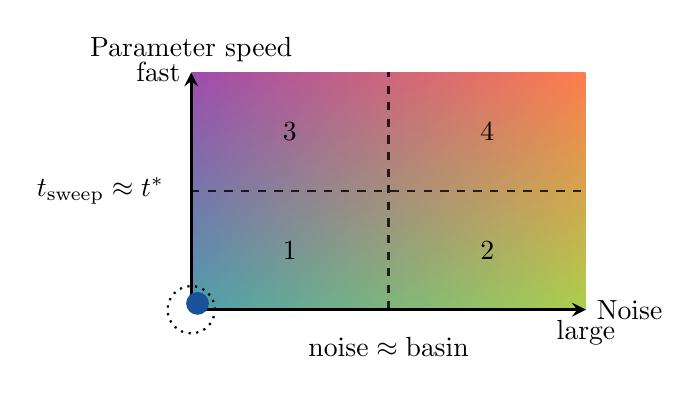
\begin{tikzpicture}
		\draw (0,0) node[rectangle, thin,left color=blue!90, right color=orange!90,shading angle=90,anchor=south west, minimum height=3cm,minimum width=5cm,opacity=0.7] (R1) at (0,0){};
		\draw (0,0) node[rectangle, thin,left color=green!80, right color=red!80,shading angle=180,anchor=south west, minimum height=3cm,minimum width=5cm,opacity=0.4] (R1) at (0,0){};
		\draw [->,opacity=1,very thick](R1.south west) node[below] {} -- (R1.south east)  node[right] {Noise} node[below] {large};
		\draw [->,opacity=1,very thick](R1.south west) node[left] {} -- (R1.north west) node[above] {Parameter speed} node[left] {fast} ;
		%\node (a) at (0.38,0.38) {};
		\draw [dashed,opacity=0.8,thick](R1.south) -- (R1.north) node {} ;
		\draw [dashed,opacity=0.8,thick](R1.west) -- (R1.east)  node {};
		%	\node[circle,draw,minimum size=10cm] (a) at (0,0) {};
		\node (a) at (0.08,0.08) {};
		\draw [dotted,thick] (R1.south west) circle [radius=0.3cm,draw=black] ;
		\filldraw [blue!70!green!80!black!90,thick] (a.center) circle [radius=0.13cm,draw=black];
		\node (e) at ($(R1.south west)!0.5!(R1.center)$) {$1$};
		\node (e) at ($(R1.south east)!0.5!(R1.center)$) {$2$};	
		\node (e) at ($(R1.north west)!0.5!(R1.center)$) {$3$};	
		\node (e) at ($(R1.north east)!0.5!(R1.center)$) {$4$};
		\node (a) at (R1.south) {};
%		\node (b) [below=0.1cm of a]  {$\sigma\sqrt{\frac{1}{2M}}\approx \mathcal{B}$};
		\node (b) [below=0.1cm of a]  {$\mathrm{noise} \approx \mathrm{basin}$};
		\node (a) at (R1.west) {};
%		\node (b) [left=0.1cm of a]  {$\frac{1}{||M||}\int \frac{d\la}{c_{\la}} \approx 1$};
		\node (b) [left=0.1cm of a]  {$t_{\mathrm{sweep}} \approx t^*$};
	\end{tikzpicture}
	\caption{We focus on slow change of parameters and small additive noise\footnote{CSD early warning work better for small noise. As with r-tipping, there will be a definition for the noise related to the tipping and another related to the goodness of the CSD theroy application.}.}        
	\label{fig: noise_transition}
\end{figure}
 
We need to develop a definition to quantify 'small' and 'slow' in this case, when the bifurcation implies a change of sign in the real eigenvalue of the fixed point. 
 
Figure \ref{fig: noise_transition} shows an example of the case we want to study (blue circle). 
In this example a 'slow' or 'adiabatic' augmented stochastic system (ASS\footnote{best acronym ever}) is only well defined in a small area, where noise is small enough for the system to not tip outside the basin far from the bifurcation, but also to be able to approximate the system being close to the equilibrium. On the other hand, we want the parameter to move slowly enough for R-tipping to not be a main mechanism of tipping, and to have the system bifurcate close to the expected parameter \citep{Marconi2020a}.%, but also to consider the noise at an equilibrium state and not have significant delays in tipping 

This defines three main areas:
\begin{enumerate}
	\item Slow parameter and low noise: The system is approximately adiabatic\footnote{In the sense of being able to use the results for $M=cte$.} without actually evolving the system step by step in the control parameter, or without any noise. In this case the main mechanism of tipping is attributed mainly to B-tipping. 
	
	\item Slow parameter and large noise: In this case the system evolves slowly but the noise is comparable or larger than the basin of attraction of $x^*$, so N-tipping is a dominant tipping mechanism and there could be a high presence of intermittency between stable states.
	
	\item Fast parameter and low noise: The system can have R-tipping and as we will see, the variance can be affected by the sweeping parameter, which can lead to delays in warnings. The behavior after the bifurcation can also be drastically different depending on the kind of bifurcation.
	\textcolor{red}{Since fast moving parameters can decrease noise, It is not clear if the high noise and high speed could lead to a different behavior of the system.}

	\item \textcolor{red}{it is not completely clear if there is a fourth case or just three}
\end{enumerate}  

Of course these distinctions are actually a part of a spectrum in the ASS system, since if a basin volume decays to zero at the bifurcation, the noise can always tip the system some time before the bifurcation of the deterministic backbone, no matter how small the noise might be. 
On the other side, a sweeping parameter will always move fast close to the bifurcation point, as the characteristic time of the system becomes infinite at the bifurcation. Thus, at some point, it will become large compared to the timescale of the sweeping and the changing parameter speed will become a relevant timescale of the system.

We can also put this in terms of tracking: if $dx^*/d\la \neq0$ then, close enough to the bifurcation, eq.\eqref{eq:Ashwin_track} cannot hold unless\footnote{From \cref{label} if the basin goes to $0$ as the bifurcation approaches, then $R\rightarrow 0$ since $R\leq \mathcal{B}$, while $d_t x^*/M\rightarrow \infty$.} $R=\infty$. 

In other words, there is no such thing as 'low' noise and 'slow' parameter near enough a critical bifurcation. 
However, we still need some definition of adiabatic, which in turn might help us to define when we are close to a tipping zone. 


                     



%\begin{figure}[htb]
%	\centering
%	\begin{tikzpicture}
%		\draw [->,opacity=1](0,0) -- (3.2,0)  node[right] {Noise};
%		\draw ->,opacity=1](0,0) -- (0,3.2) node[above] {Parameter speed} ;
%		\draw (0,0) node[rectangle, thin,left color=blue!80, right color=red!80,shading angle=130,anchor=south west, minimum height=3cm,minimum width=3cm,opacity=0.6] {} {};
%		\node (a) at (0.3,0.3) {};
%		\draw [dashed,opacity=0.8](1.5,0) -- (1.5,3) node {} ;
%		\draw [dashed,opacity=0.8](0,1.5) -- (3,1.5)  node {};
%		%	\node[circle,draw,minimum size=10cm] (a) at (0,0) {};
%		\filldraw [blue] (a.center) circle [radius=0.1cm,draw=black];
%	\end{tikzpicture}
%	\caption{We focus on slow change of parameters and small additive noise.}        
%	\label{fig: noise_transition}
%\end{figure}








%\begin{center}
%	\begin{tikzpicture}[scale=1.5]
		%		% Draw axes
%		\draw [<->,thick] (-2,2) node (yaxis) [above] {$Noise$}
	%	\draw [<->,thick] (-2,2) node (xaxis) [right] {$\dot\theta$};
		%		% Draw two intersecting lines
		%%		\draw (0,0) coordinate (a_1) -- (2,1.8) coordinate (a_2);
		%%		\draw (0,1.5) coordinate (b_1) -- (2.5,0) coordinate (b_2);
		%		% Calculate the intersection of the lines a_1 -- a_2 and b_1 -- b_2
		%		% and store the coordinate in c.
		%%		\coordinate (c) at (-1,-1)
		%%		\draw[dashed] (yaxis |- c) node[left] {}
		%%		-| (xaxis -| c) node[below] {};
		%%		\coordinate (c) at (intersection of (yaxis) and ());
		%		% Draw lines indicating intersection with y and x axis. Here we use
		%		% the perpendicular coordinate system
		%%		\draw[dashed] (yaxis |- c) node[left] {$y'$}
		%%		-| (xaxis -| c) node[below] {$x'$};
		%		% Draw a dot to indicate intersection point
		%%		\fill[red] (c) circle (2pt);
%	\end{tikzpicture}
%\end{center}


\begin{figure}[htbp]
	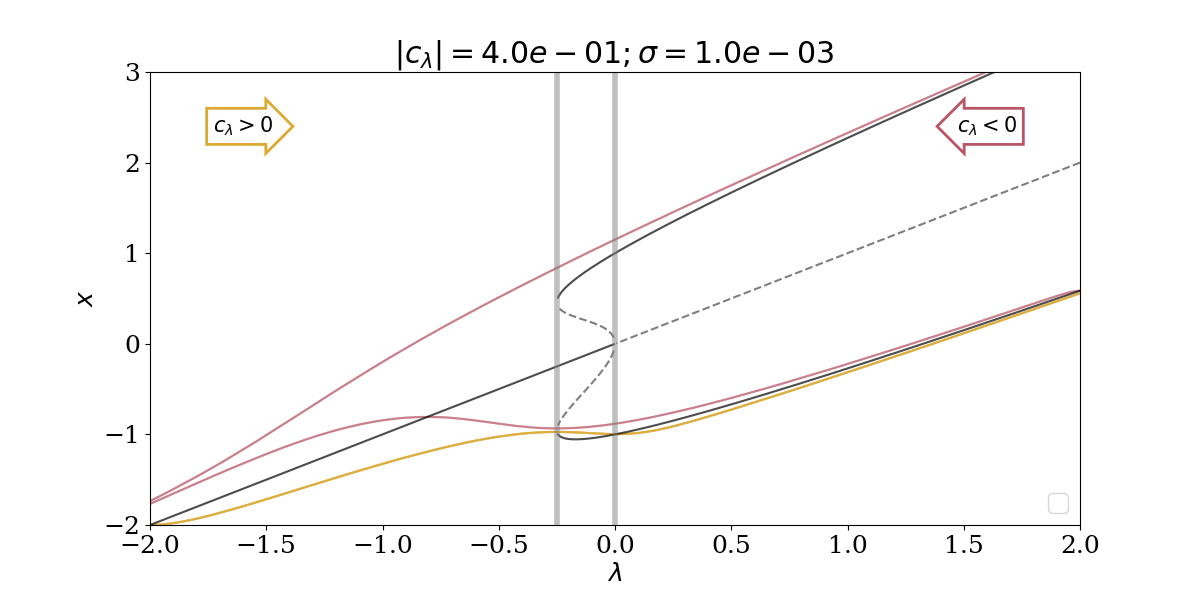
\includegraphics[width=0.49\linewidth]{Images/Metrics/spectrum_cases/slanted_subpitch_fast}
	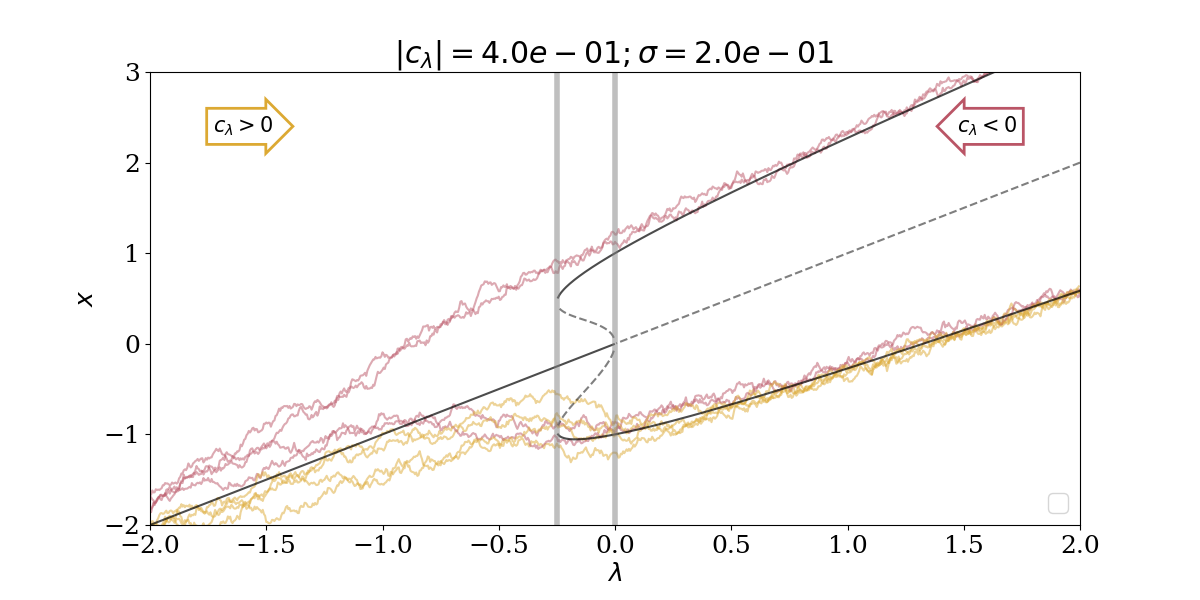
\includegraphics[width=0.49\linewidth]{Images/Metrics/spectrum_cases/slanted_subpitch_fastnoise}\\
	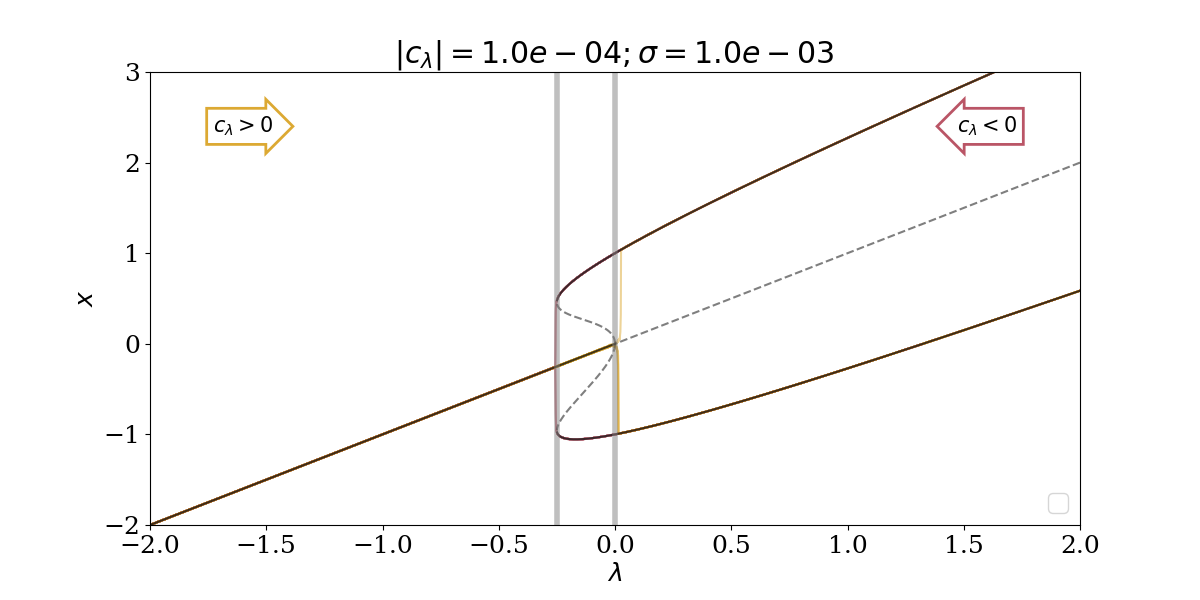
\includegraphics[width=0.49\linewidth]{Images/Metrics/spectrum_cases/slanted_subpitch_adiab}
	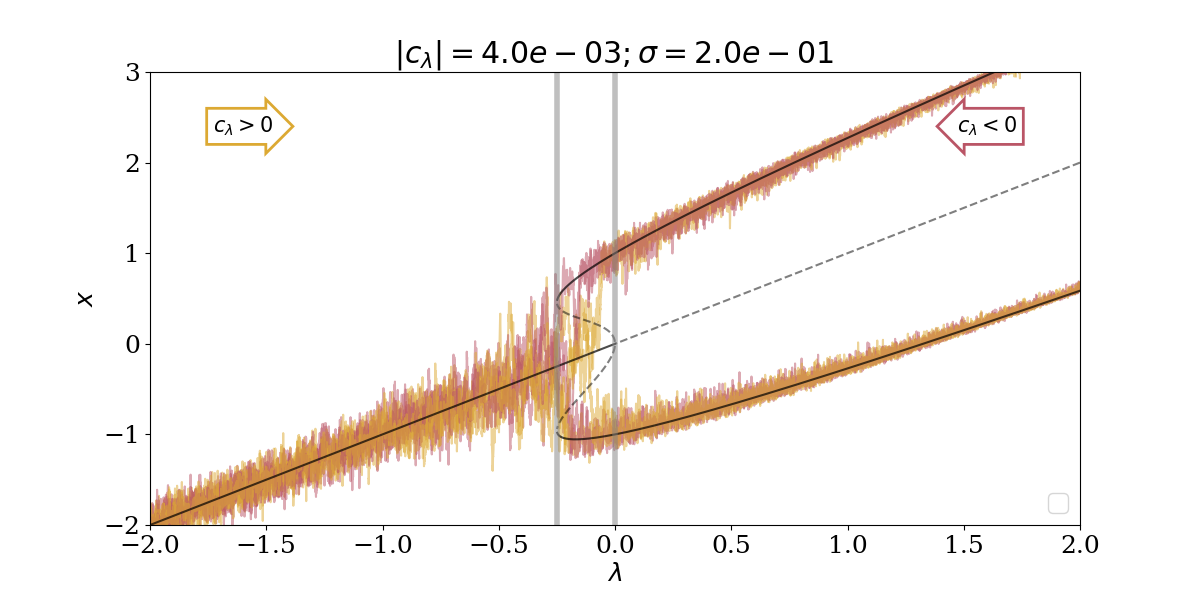
\includegraphics[width=0.49\linewidth]{Images/Metrics/spectrum_cases/slanted_subpitch_noise}
	\caption{Stochastic trayectories of the subcritical pitchfork $dx=\la (x-\la)+(x-\la)^3-(x-\la)^5 dt+\sigma dW$, with fast or slow swiping parameter $\dot{\la}=\left\{0.4,0.004\right\}$ and big or small noise at the bifurcation $\sigma=\left\{0.2,0.01\right\}$. The gray lines mark the bifurcation points for the respective branches.}
	\label{fig: cases}
\end{figure}








\subsection{Defining an adiabatic sweeping}

 \cite{Perryman2014a}  called adiabatic  systems that close track their autonomous equilibria.
  However, we will show this is not enough to define 'slow' in this case, though in the end, the threshold will still be compatible. 

We can consider one of the simplest cases for a dynamical system

%\begin{equation}
%	\begin{aligned}
	%		d x&=\lambda x\,dt+\sigma\, dW,\\
	%		d \la &= c_\lambda\, dt > 0.\\
	%		\la_0 < 0.
	%	\end{aligned}
%\end{equation}

\begin{equation}
	\begin{cases}
		dx &=-\lambda x \,dt + \sigma\, dW,\\
		d \lambda &= c_\lambda\, dt <0,\\
		\lambda_0 &> 0.
	\end{cases}
\label{eq: simplecase}
\end{equation}

In this case there is only one stable equilibrium, $x^*=0, \quad \forall \la >0 $, and all other quantities are trivial to calculate, $M=-\la$.
Close tracking is trivially satisfied since $\frac{dx^*}{dt}=0$, but we can still define a time scale related to the changing parameter  which can be compared to the timescale of the system $t^*=-1/M$.
A simple dimensional analysis would make it tempting to choose $\la/c_\la$ as a timescale, but this cannot be the case since the timescale cannot depend on the value of $\la$.

Let us consider the case of a control parameter that is always sweeping in the same direction, that is to say, if $c_\lambda\neq 0 \quad \forall \, t$ then  $\lambda(t)$ is monotonic (inyective) in time and we can write 

\begin{equation}
	t-t_0=\int_{\lambda_0}^{\lambda(t)} \frac{d\lambda}{c_\lambda}
\end{equation}

So we can write the variance in \cref{eq: ST_variance} as 
\begin{equation}
	\mathrm{Var}[x]=\frac{\sigma^2}{2 ||M(x^*,\lambda)||}\left( 1-e^{-2M(x^*,\lambda)	\int_{\lambda_0}^{\lambda(t)} \frac{d\lambda}{c_\lambda}}\right) 
	\label{eq: ST_variance_swip}
\end{equation}
This makes explicit the dependence of the variance on the sweeping speed $c_\lambda$, though it still has a 'memory' of when integration 'started'. 

 With this we can have a first definition of parameter moving adiabatically: the realization ensemble statistics needs to follow the dependence of the equilibrium variance \cref{eq: ST_variancelim}. 
From eq.\eqref{eq: ST_variance_swip}, we can see that this happens when 
\begin{equation}
	e^{-2M(x^*,\lambda)	\int_{\lambda_0}^{\lambda(t)} \frac{d\lambda}{c_\lambda} }\approx 0
	\label{eq: ST_adabatic_condition}
\end{equation}

Since all this development assumes there is a stable equilibrium $x^*$, if there is a bifurcation at $\lambda_c$ we can ask ourselves what happens when $\lambda_f=\lambda_c$.


However, first let us consider the case where at $t_0$ the system has been evolving for a long time in the past\footnote{In appendix  \ref{apx:variance_contradiction} we explain briefly a possible contradiction on the effect of the variance when the parameter moves fast.}, longer than several correlation times and relaxation times. %for whatever values this might take for the past values of the control parameter. 
Then, the 'initial' value at $t_0, \la_0$ is actually a value belonging to an ensemble with variance $Var(t_0)=\sigma^2/2\la_0$ since we consider an initial condition defined in an equilibrium state. 

In this case we could argue that the system has 'forgotten' where it came from\footnote{Similar arguments are made also in \citep{...}}, due to the stochastic process and we can drop that part of the integral\footnote{The dependence of the initial value is forgotten as $\int^{\la_f}_{\la_0}\frac{d\la}{c_\la}=F(\la_f)-\cancelto{}{F(\la_0)}$}:
\begin{equation}
	\mathrm{Var}[x]=\frac{\sigma^2}{2 ||M(x^*,\lambda)||}(1-e^{-2M(x^*,\lambda)	\int^{\lambda(t)} \frac{d\lambda}{c_\lambda}})
	\label{eq: ST_variance_sweep2}
\end{equation}
and only evaluate the primitive of $1/c_\la$ at $\la(t)$.

Then $-2M(x^*,\lambda) \int^{\lambda(t)} \frac{d\lambda}{c_\lambda} $ defines a timescale (or equivalently a $\la$ value) at which the system starts deviating from the expected adiabatic value from eq.\eqref{eq: ST_variancelim}.


We will define an adiabatic sweep as one where

\begin{equation}
	e^{-2M(x^*,\lambda)	\int_{\lambda_0}^{\lambda(t)} \frac{d\lambda}{c_\lambda} }<1
\end{equation}

for which we ask 

\begin{equation}
 -2M(x^*,\lambda)	\int_{\lambda_0}^{\lambda(t)} \frac{d\lambda}{c_\lambda} >1
\end{equation}
\textcolor{red}{Am i missing some absolute value ?}


rewritten as  

\begin{equation}
	\tcbhighmath{
	\int^{\lambda(t)} \frac{d\lambda}{c_\lambda} >-\frac{1}{2M(x^*,\lambda)}=\frac{t^*(\lambda)}{2}
}
	\label{eq:noiseadiab}
\end{equation}

Therefor the adiabatic swiping in terms of noise happens when a timescale of the swiping  $\int^{\lambda} d\lambda / c_\lambda$ is smaller than half the relaxation time. 

In the case of a parameter changing at a constant rate ($c_\la(t,\la)=c_\la$), we get 
\begin{equation}
	\frac{\lambda}{c_\lambda} >-\frac{1}{2M(x^*,\lambda)}
	\label{eq:noiseadiab_cte}
\end{equation}

Another way to look at this result is that there is no 'moving slow' near some bifurcations. In this case, for a parameter with constant speed ($c_\lambda$) there is always an open set that contains the stable branch, where the equilibrium results are no longer valid. We are going to come back to this idea after we recall some results from R-tipping theory by \cite{Ashwin, the other one}.

However this does give us a possible definition of adiabatic shift for some region of parameters that will depend on the sweeping.  



\begin{figure}[htb]
	\centering
	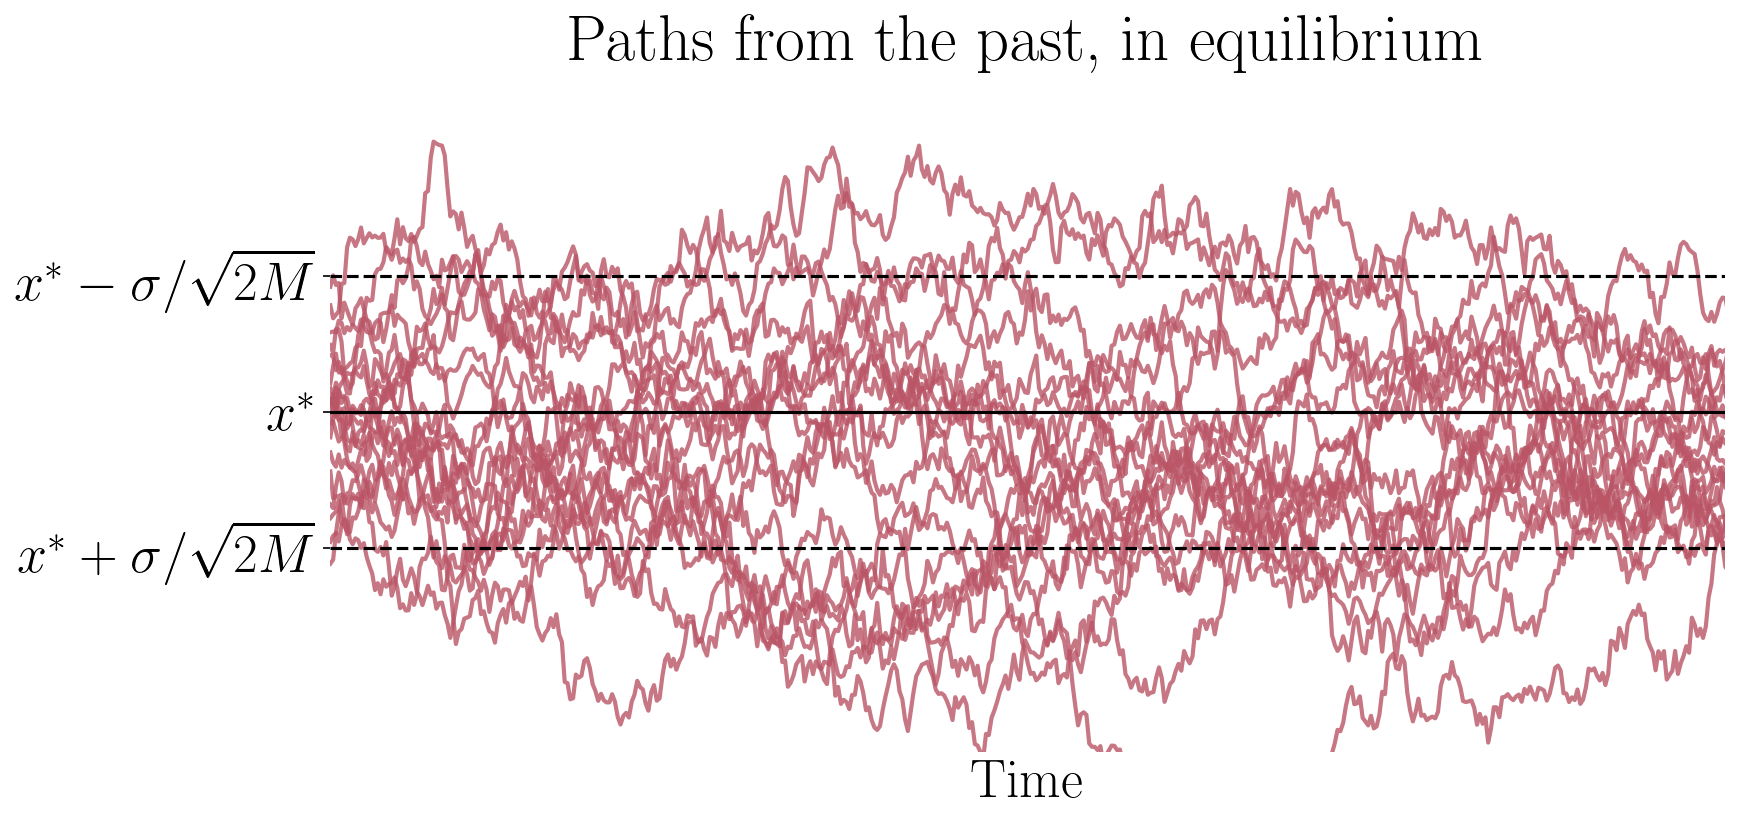
\includegraphics[width=0.9\linewidth]{Images/Metrics/diff_init2}\\
	\caption{ Example of 20 integrations of \cref{eq: simplecase} with $\la=2$ and $c_\la=0$, where the initial condition are sampled from the expected equilibrium balance.}
	\label{fig:diffinit}
\end{figure}

Figure \ref{fig:diffinit} shows an example of 25 evolutions of \cref{eq: simplecase} with $\la=2$ and $c_\la=0$, assuming the initial condition come from  a far past so they are sampled from the expected equilibrium variance in \cref{eq: ST_variancelim}. 

\begin{figure}[tbp]
	\centering
	\includegraphics[width=\linewidth]{"../Programing Proyects/EE indicators/Simulations with pdfs to test/Stochastic equations/SDE tests jupyter/image_variance_speed/Good_test/toghether/000_variance_test_speed_toghether"}
	\caption{Comparison between the expected variance and mean, to the measured ones, both for an ensemble of 300 trajectories (orange) and for a single trajectory (blue). Theoretical expected values are shown in dashed black lines, the vertical red line marks the adiabatic threshold as defined in \cref{eq:noiseadiab} and the gray line marks the bifurcation point. This example shows sweeping rate $c_{\la}=2$ resulting in a fast sweeping region for $\la=[0,2.8]$.}
	\label{fig:000variancetestspeedtoghether}
\end{figure}


To test our hypothesis of using the criteria of \cref{eq:noiseadiab} as the limit to consider a slow sweeping of the parameter, we realize 300 integrations starting from initial conditions as shown in \cref{fig:diffinit} and we evolve the system from $\la_0=3$ to $\la_f=0.001$
 at different speeds, and calculate for each speed the variance and the mean for the ensemble of trajectories, and also for a  singular trajectory.
 
 Figure \ref{fig:000variancetestspeedtoghether} shows in orange the variance and the mean calculated from the ensemble values after a nonparametric block bootstraping after 500 bootstraps and using 70\% of the data length for each bootstrap. The values for calculated by bootstrapping the single trajectory are shown in blue.
 The top plot shows the variance and the expected equilibrium variance from  \cref{eq: ST_variancelim} in dashed black line.
 The middle lot shows the variance normalized to the expected  equilibrium variance from \cref{eq: ST_variancelim} to make more evident the deviation from the equilibrium.
 The bottom plot shows the mean, which is expected to be $0$, and in gray shows an example of a single raw trajectory.
 The vertical red line indicate the threshold defined by \cref{eq:noiseadiab}.
 This example shows sweeping rate $c_{\la}=2$ resulting in a fast sweeping region for $\la=[0,2.8]$
 
\begin{figure}[tbp]
	\centering
	\includegraphics[width=1\linewidth]{"../Programing Proyects/EE indicators/Simulations with pdfs to test/Stochastic equations/SDE tests jupyter/image_variance_speed/Good_test/toghether/014_variance_test_speed_toghether"}
	\caption{Same analysis as in \cref{fig:000variancetestspeedtoghether}. This example shows a slower sweeping rate $c_{\la}=0.0074$ resulting in a fast sweeping region for $\la=[0,0.2]$.}
	\label{fig:014variancetestspeedtoghether}
\end{figure}


Figure \ref{fig:014variancetestspeedtoghether} shows the same information, for a slower sweeping were in can be seen that ensemble and single trajectory statistics behave similarly until close to the to the adiabatic threshold in with  \ref{fig:000variancetestspeedtoghether}.

From this test we can see that   \cref{eq:noiseadiab} in this particular case predicts qualitatively when the ensemble statistics deviate from the expected values.
Therefore the sweeping speed is clearly relevant even in cases when the system trivially close tracks $x^*$.

For completeness, in \cref{fig:stats} we analyze the EWS of interest for the case where  we don't sweep the control parameter but we evolve it by steps. That is, we analyze each case for a constant value of $\la$, then we move to the next value $\la-\Delta \la$ using the last value as initial condition, waiting for a transient time, and we re-do the analysis. 
To increase the resolution near the bifurcation, the values of $\la$ are logarithmically spaced between $\la_0=3$ (check) and $\la_f=0.001$. 

Each point the is result of calculating the EWS by bootstraping like in the previous case, for an original sample of 3690 point.
\begin{figure}
	\centering
	\includegraphics[width=0.9\linewidth]{"../Programing Proyects/EE indicators/Simulations with pdfs to test/Stochastic equations/SDE tests jupyter/image_variance_speed/skipping/stats"}
	\caption{Analysis of the EWS for the autonomous case of \cref{eq: simplecase} with a stepped evolution of $\la$. To increase the resolution near the bifurcation, the values of $\la$ are logarithmically spaced.  }
	\label{fig:stats}
\end{figure}


In appendix \ref{apx:sameinit} we show the same analysis for the case where the initial conditions of the ensemble are all the same, thus keeping the information of the 'past'. In this case \cref{eq:noiseadiab} also marks a reasonable timescale for the memory of the system.



\section{Tracking timescale, and loss of symmetry in the augmented system}

It should be noted that, when investigating the ASS system, autonomous systems that are equivalent (same normal form), are not equivalent anymore. 

To exemplify this, we can look the transcritical bifurcation from the system
\begin{equation}
	\begin{cases}
		dx & = x(x-\la)dt+\sigma dW\\
		d\la & =c_\la dt
	\end{cases}
	\label{eq: tranc}
\end{equation}
whose non-autonomous equilibria are defined as $x^*=\left\lbrace 0,\la\right\rbrace $, with a bifurcation at $\la=0$ where the equilibria change stability. The LDR for the stable equilibria in this system is always $M=\la$.

We could do a translation of this system as  
\begin{equation}
	\begin{cases}
		dx & = (x-\la)(x-2\la)dt+\sigma dW\\
		d\la & =c_\la dt
	\end{cases}
\label{eq: tranc_sl}
\end{equation}
now the deterministic autonomous backbone of this systems are the same, except that the equilibria are translated by $\la$, $x^*=\left\lbrace \la,2\la\right\rbrace $; and $M=\la$ for all the stable equilibria. 

However, for \cref{eq: tranc}, the stable equilibria $x^*={0}$ has not rate-dependence, furthermore, after it turns unstable it continues along the same path as $x^*_u={0}$. 
If we look at what happens to the ASS system (\cref{fig:transcr}), with $c_\la=0.02$ and $\sigma=0.01$, the paths generated from sweeping $\la$ from positive to negative (red) have an equal chance of diverging or going to the new equilibrium. 
While the  paths generated from sweeping $\la$ from negative to positive (yellow) are all will not diverge since the deviation due to the rate keeps them completely contained on the basin of the stable equilibrium.  

\begin{figure}[htb]
	\centering
	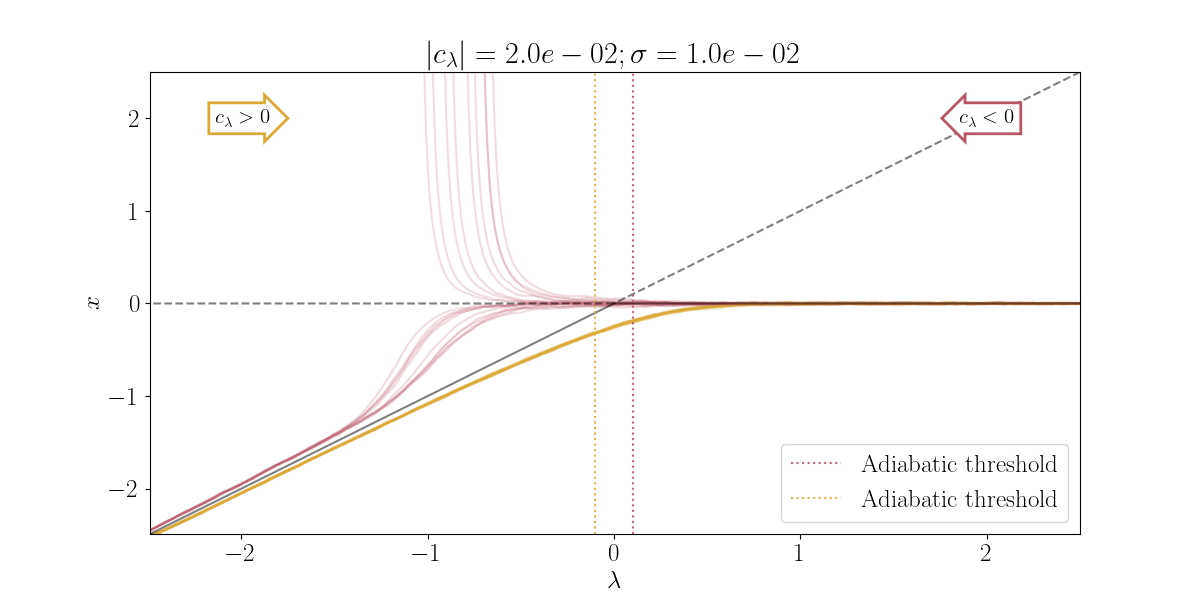
\includegraphics[width=\linewidth]{Images/Metrics/nonnormality/transcr}
	\caption{Integration of 20 different paths of \cref{eq: tranc} sweeping from negative to positive $\la$ (yellow) and vice-versa (red), with $c_\la=0.02$ and $\sigma=0.01$. Vertical dotted lines identify the adiabatic limit from \cref{eq:noiseadiab} for the respective branches. }
	\label{fig:transcr}
\end{figure}

If we look to what happens to \cref{eq: tranc_sl}, for the same sweeping speed and the same noise, all the trajectories in the positive to negative sweep diverge, and do so faster than in the previous case. 

\begin{figure}[htb]
	\centering
	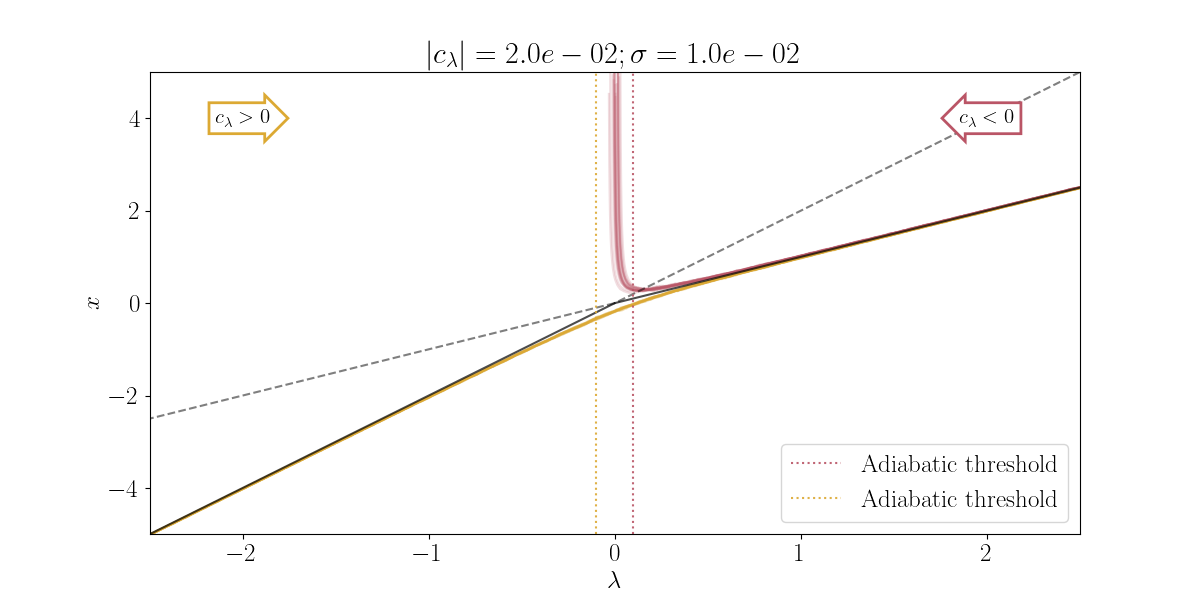
\includegraphics[width=\linewidth]{Images/Metrics/nonnormality/transcr_sla}
	\caption{Integration of 20 different paths of \cref{eq: tranc_sl} sweeping from negative to positive $\la$ (yellow) and vice-versa (red), with $c_\la=0.02$ and $\sigma=0.01$.  Vertical dotted lines identify the adiabatic limit from \cref{eq:noiseadiab} for the respective branches.}
	\label{fig:transcrsla}
\end{figure}

Now there is also a deviation due to the rate of sweeping in the other branch, and all the trajectories get pushed towards the unstable basin before the bifurcation happens. 

The difference in tipping time in this case is also affected by the rate. 
In \cref{fig:transcr}, near after the bifurcation, the systems stays doing a Brownian motion around the unstable equilibria, and since the local potential landscape is very flat $M\approx 0$ it will diverge once a the random walk takes it far away enough of the hill, and/or the hill becomes concave enough to repel the system.

While in \cref{fig:transcrsla}, even if the system does not completely tip before the bifurcation, the divergence of the trajectory will be faster as in this case the system cannot do a random walk in the unstable equilibrium after the bifurcation since the equilibrium itself moves away. 

We add in appendix \ref{apx:simetrictranscrit} a full symmetric case as a further example, plus a similar example for the normal form of a subcritical pitchfork bifurcation and a translated version.

This effect can have important implications in the reversibility of a system after a bifurcation. If we consider a system that evolved slowly from negative to positive values of the control parameter, when trying to recover the system to the old behavior, retracting fast is worst that retracting slow and the system might tip before showing signs of slowing down. 

\begin{figure}[htb]
	\centering
	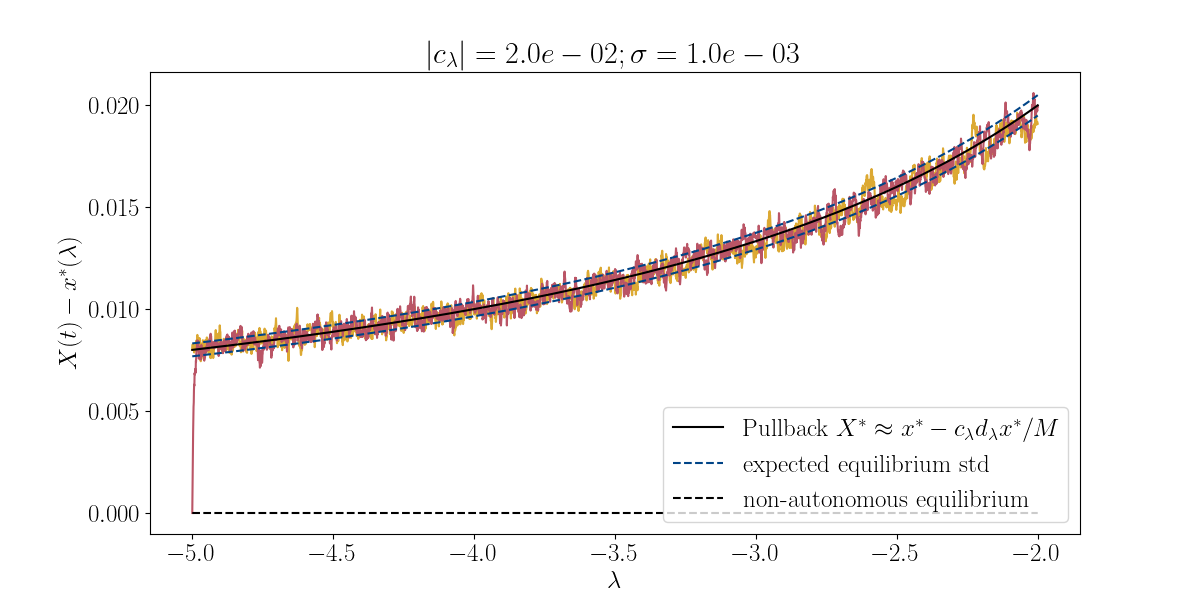
\includegraphics[width=1\linewidth]{Images/Metrics/nonnormality/deviation_trancr}
	\caption{Example of close tracking on \cref{eq: tranc_sl} for a slow variation of the control parameter. The dashed line represents the stable equilibrium ($x^*$) which is set to zero for plotting purposes. Two trajectories are displayed. The red has an initial condition at $x^*$ while the yellow starts at the expected correction from the linear instantaneous lag. The solid black line is the expected path from the linear correction and the dashed lines are the expected standard deviation from \cref{eq: ST_variancelim}. }
	\label{fig:deviationtrancr}
\end{figure}

Inspired by the results of \cref{eq:noiseadiab} we propose
\begin{equation}
		\tcbhighmath{
	t_{\mathrm{sweep}}=\int \frac{d\lambda}{c_\lambda} 
}
\end{equation}
as a characteristic timescale for the sweeping parameter. I should be noted that the integral is not defined when $c_\la=0$ being consistent with not having a timescale if there is no sweeping.
So we propose to compare this timescale  to the relaxation timescale results in  
\begin{equation}
		\tcbhighmath{
	\int  \frac{d\la}{c_\la} > -\frac{1}{||M||}.}
\end{equation}
We will show that this timescale will define the range of validity of the approximation of the instantaneous lag and gives a clear definition for close tracking in terms of the control parameter speed and the attraction of the stable equilibrium. 
As a bonus, it also gives a regime on which the  effective tipping radius $R$ from \cref{eq:Ashwin_track} is approximately the same as the basin radius.

Using as example the negative stable branch of \cref{eq: tranc_sl}, \cref{fig:deviationtrancr} display the deviation from the expected linear instantaneous lag correction as a function of the sweeping rate $c_\lambda$, for the range where we still consider a slow sweeping. The dashed line is the detrended stable branch $x^*=2\la$, the solid black line is the expected deviation due to the instantaneous lag, surrounded by blue dashed lines showing the expected equilibrium standard deviation from \cref{eq: ST_variancelim}. The red trajectory has an initial condition on the $x^*$ branch while the yellow trajectory has an initial condition on the expected position due to the instantaneous lag.



Figure  \ref{fig:adiabrtipdef010} and \cref{fig:adiabrtipdef039} display the deviation from the expected linear instantaneous lag correction as a function of the sweeping rate $c_\lambda$ and the proximity to the bifurcation. 
Figure \ref{fig:adiabrtipdef010} shows a slower sweeping rate, where the system follows the expected variance and trajectory of the linear correction up to the dashed blue line, close to the bifurcation. 
The top plot shows the trajectory in red, the stable and unstable branches, the expected path as a  dashed-dotted line (which diverges at the bifurcation), the yellow dotted line shows the limit up to which we expect the system to close track ($\int d\la/c_\la =1/M$), and the blue line  is defined as a tighter restriction ($\int d\la/c_\la =10/M$).
The middle plot shows the same information, translated to $x^*$ for plotting purposes. 



The bottom plot shows in log scale the normalized (to the pullback attractor $X^*$) deviation from the linear instantaneous lag correction. 
Here we can see that the criteria ($\int d\la/c_\la =1/M$) matches an order 0 deviation from the expected value, while ($\int d\la/c_\la =10/M$) is gives a deviation between $1\%$ and $10\%$ of the expected value. 


\begin{figure}[htb]
	\centering
	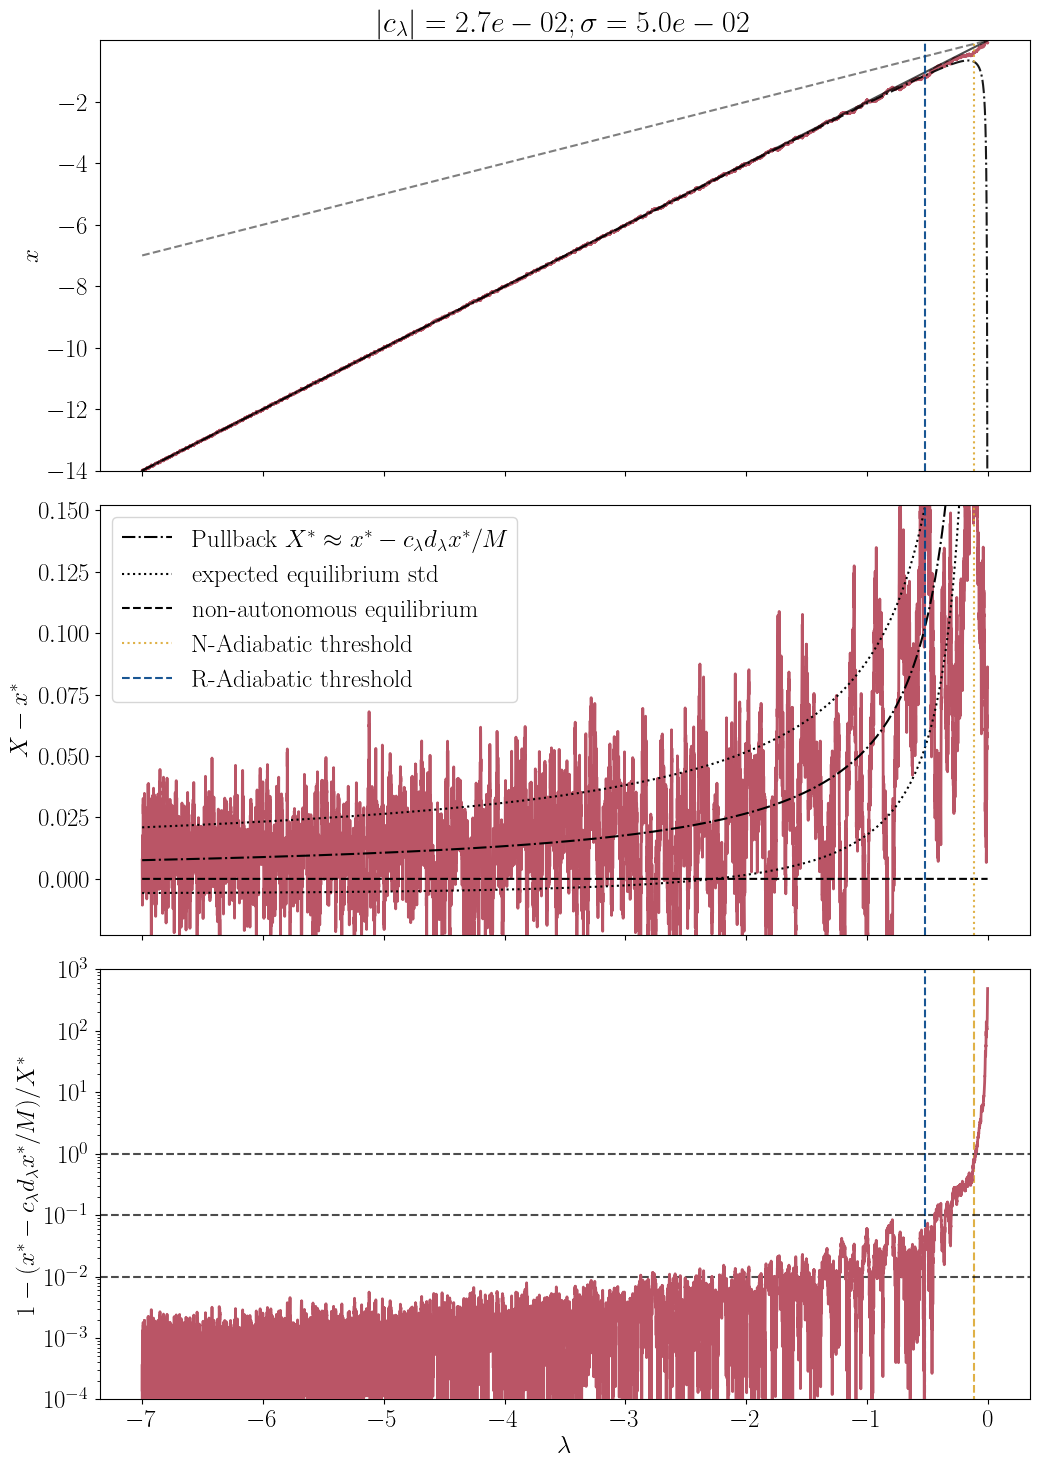
\includegraphics[width=0.9\linewidth]{Images/Metrics/traking/adiab_rtip_def010}
	\caption{Slower sweeping example.  }
	\label{fig:adiabrtipdef010}
\end{figure}

\cref{fig:adiabrtipdef039} shows a faster sweeping rate. In this case, the system deviates from the expected linear correction much faster. However as we can see from the bottom plot, the same features are retained, where the criteria ($\int d\la/c_\la =1/M$) matches an order 0 deviation from the expected value, while ($\int d\la/c_\la =10/M$) is gives a deviation between $1\%$ and $10\%$ of the expected value. 

\begin{figure}[htb]
	\centering
	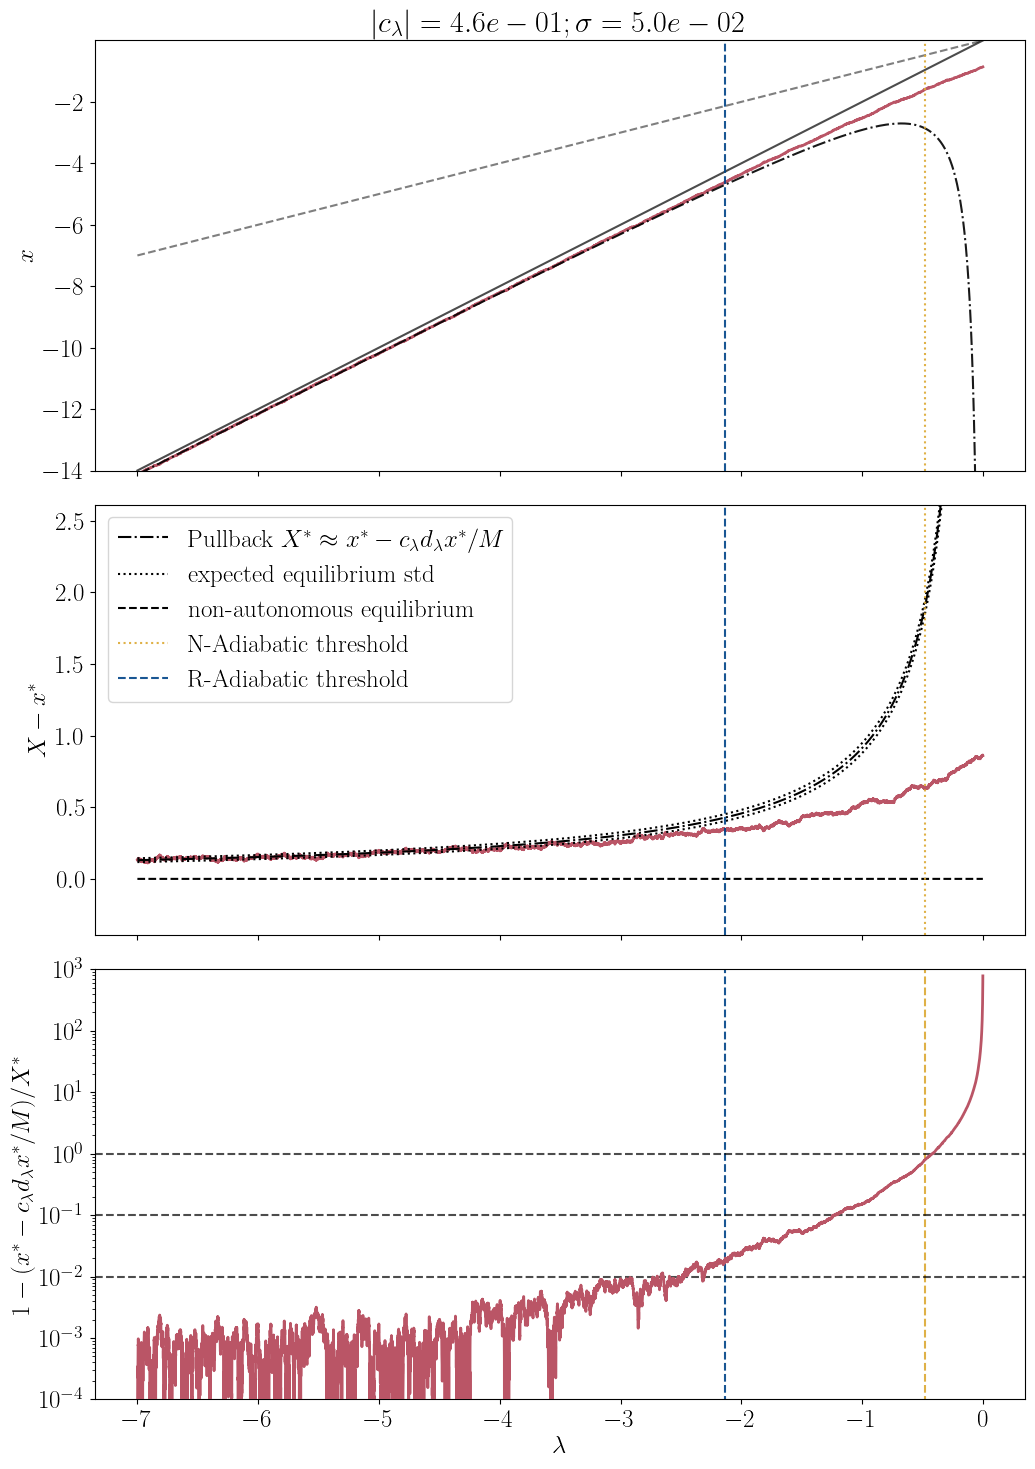
\includegraphics[width=0.9\linewidth]{Images/Metrics/traking/adiab_rtip_def039}
	\caption{Faster sweeping example.}
	\label{fig:adiabrtipdef039}
\end{figure}

Thus comparing the scale defined by $\int d\la/c_\la =1/M$ seems to give a reasonable scale to the define a threshold for slow variation in terms of close tracking, defined as the pullback attractor following the linear instantaneous lag.
This is also a reasonable definition for adiabatic sweeping since it relates to the definition for adiabatically in the stochastic sense ($\int d\la/c_\la =1/2M$)
and it is related to following a path calculated by assuming the $M$ does not change. 
In other words, this scale defines up to which point the control parameter changes slow enough that we might consider $M$ (or conversely, the return rate) at each point in time, the same as in the autonomous case. 
Again, close enough to the bifurcation this assumption will always fail. This adiabatic definitions define where (or when) is close enough for each sweeping speed. 



	\section{adiabatic number}

A natural way to say that a parameter is being sweept slowly when  the system is close to a stable attractor would be to say that, if the control parameter at $t_i$ is $\lambda_i$, then after a relaxation time $t^*_i=-1/M(\la_i)$ the system moves to a state given by  $\lambda_i+\delta \la$ on which the relaxation time has not change significantly. 

Thus we want $\Delta M=M_f-M_i$ to be small, with $M_f=M(\lambda_i+\delta \la)$, and $M_i= M(\lambda_i) $.

To quantify this we choose wither of the follow adimensional quantities:

\begin{equation}
	\begin{aligned}
		\xi_i&=\frac{\Delta M}{M_i}=\frac{M_f}{M_i}-1 \\
		\xi_f&=\frac{\Delta M}{M_f}=1-\frac{M_i}{M_f}
	\end{aligned}
	\label{eq:xi}
\end{equation}

We will call this quantities the adiabatic number of the augmented system. 

And they have the following properties:
\begin{itemize}
	\item They are positive if the system becomes locally more stable, since the relaxation times decreases. 
	\item They are zero if the system does not change stability. Thus, the are zero if the system is not being swiped.
	\item They are negative if the system losses stability.
\end{itemize}

In particular they take values in given intervals $\xi_f  \in (-\inf,1)$, $\xi_i  \in (-1,\inf)$.





\tikzmath{ int \k ; }
\begin{figure}
	\centering
%	\begin{tikzpicture}
%		\node (time) at (11,0)  [right]{$t$};
%		\draw [->,very thick,black](0,0) -- (11,0);
%		\node[above,left] at (0,3) {a)};
%		\foreach \i in {0,...,4}
%		{ \draw (2*\i,0) node[rectangle, thin,left color=col2, right color=white!,shading angle=180,anchor=south west, minimum height=3cm,minimum width=2cm,opacity=0.2+\i*(1-0.2)/9] () {}; }
%		\foreach \i in {0,...,5}
%		{ \filldraw (2*\i,0) circle [circle,black,fill=black,align=center,radius=0.05cm] ; }
%		\node[below] (a) at (0,0) [center,below]{$t_i$};
%		\node[below] (b) at (2,0) [center,below]{$t_{i+1}$};
%		\node[below] (b) at (4,0) [center,below]{$t_{i+2}$};
%		\draw [dotted , thick , black,right](6,-0.3) -- (8,-0.3);
%		\node[below] (b) at (10,0) [center,below]{$t_{n}$};
%		\tzfn[->,col1,ultra thick]{3.5*exp(-1.3*\x)}[0.1:1.5]{}[al]		
%	\end{tikzpicture}
	
	\begin{tikzpicture}
		
		\k=0;
	
		\draw (0,0) node[rectangle,  thin,left color=col2, right color=white!,shading angle=180,anchor=south west ,anchor=south west, minimum height=3cm,minimum width=1.1 cm,opacity=1] () {};
		\draw (1.1,0) node[rectangle,  thin,left color=col2, right color=white!,shading angle=180,anchor=south west ,anchor=south west, minimum height=3cm,minimum width=1.2 cm,opacity=0.9] () {};
		\node[below] (a) at (0,0) [center,below]{$t_i$};
		\node[below] (b) at (1.1,0) [center,below]{$t_{i}+t_i^*$};
%		\node[below] (b) at (2,0) [center,below]{$t_{i+2}$};
		\draw [dotted , thick , black,right](3.3,-0.3) -- (5,-0.3);

		\tzfn[->,col1,ultra thick]{3.5*exp(ln(.1/3.5)*\x)}[0.:1.1]{}[ar]
		\tzfn[->,col1,ultra thick]{3.5*exp(ln(.1/3.5)/1.1*(\x-1.1))}[1.1:2.3]{}[ar]		
%		
		\draw (6,0) node[rectangle,  thin,left color=col2, right color=white!,shading angle=180,anchor=south west ,anchor=south west, minimum height=3cm,minimum width=2cm,opacity=0.5] () {};
		\draw (8,0) node[rectangle,  thin,left color=col2, right color=white!,shading angle=180,anchor=south west ,anchor=south west, minimum height=3cm,minimum width=4cm,opacity=0.3] () {};
		\node[below] (a) at (6,0) [center,below]{$t_i$};
 		\node[below] (b) at (8,0) [center,below]{$t_{i}+t_i^*$};

		\tzfn[->,col1,ultra thick]{3.5*exp(ln(.1/3.5)/2*(\x-6))}[6:8]{}[ar]
		\tzfn[->,col1,ultra thick]{3.5*exp(ln(.1/3.5)/4*(\x-8))}[8:12]{}[ar]
		\node[above,left] at (0,3) {b)};	
		
		\node (time) at (13,0)  [right]{$t$};
		\draw [->,very thick,black](0,0) -- (13,0);
		\foreach \i in {0,1.1,2.3}
		{\filldraw (\i,0) circle [circle,black,fill=black,align=center,radius=0.05cm] ; 
		};
		\foreach \i in {6,8,12}
		{			\filldraw (\i,0) circle [circle,black,fill=black,align=center,radius=0.05cm] ; 
		}
	\end{tikzpicture}
	\caption{Scheme for the definition of slow sweeping. We consider a slow sweeping if the relaxation time does not change significantly after one relaxation time $t^*$}.
	\label{fig: velocity_param3}
\end{figure}



\section{Simulation and analysis methodology.}

First an initial ($\la_0$) and final control parameter $\la_f$ are chosen, then integration step is chosen to be a fourth of the smallest expected time-scale for the autonomous system. 
In this case, for 1-dimensional systems, the smallest time-scale is chosen as $t_{min}=min (-1/2M)$ chosen as $1/2M$ since the stochastic timescale from \cref{eq: ST_variance}  instead of $1/M$, therefore this is set by the most stable point of the system\footnote{In appendix \ref{apx:param_speed_integration} an intuitive scheme is presented on why this choices of time step are also relevant for the stability of the numerical integration.}. 

Rewriting the criteria of \cite{Thompson2011a} for the windowing  and separation of scales\footnote{In \cite{Thompson2011a} the sweeping rate is, called drift rate in their paper ($\kappa_{\mathrm{drift}}$) , is defined as the average sweeping rate  of the control parameter. However this rate will have the units of the control parameter per second, while our definition has units of $1/s$ as does the LDR.}, as timescales:
\begin{equation}
	\int \frac{d\la}{c_\la} >> -\frac{1}{||M||}>> -\frac{1}{M_{\mathrm{other-scales}}}
\end{equation}
where $M_{\mathrm{other-scales}}$ refers to the other eigenvalues $m$ when the system has more dimensions. This equivalent to asking for a clear separation of timescales in the deterministic backbone, and a clear separation of timescale with the sweeping parameter that is equivalent to a slow sweeping rate. 
As we have shown, this relations can only hold far from the critical bifurcation, since no matter how it is approached, at some point the sweeping rate will be similar and then smaller than the relaxation time\footnote{Unless it is possible in some scenario to slow down the sweeping rate faster than the decay of $M$, though that case the bifurcation point will never be reached.}. 	
	
where the sampling time of the data, $\Delta t_{\mathrm{sample}}$, has to obey
\begin{equation}
	-\frac{1}{||M||} >> \Delta t_{\mathrm{sample}} >> -\frac{1}{M_{\mathrm{other-scales}}}.
\end{equation}



For the analysis, three other scales have to be chosen. A time length for the EWS signal running window calculation; and, in case of using a detrending, a scale for the running detrending window and a bandwidth for the Gaussian kernel of the detrending window. 
Since at the critical bifurcation, the auto-correlation converges to one, the correlation length diverges. 
Therefore, any analysis window close enough to the bifurcation will be too small.

So as before, any windowing we choose can only hold for a range of parameters at some distance to the bifurcation

The detrending for the analysis of the EWS is done by a moving average with a gaussian kernel with bandwidth ($\mu$), such that:
\begin{equation}
	\int \frac{d\la}{c_\la} >> \mu >> -\frac{1}{||M||}
\end{equation}
and the EWS analysis window
\begin{equation}
	\int \frac{d\la}{c_\la} >> (2m+1)\Delta t 
\end{equation}

In particular we choose
\begin{equation}
	-\frac{1}{2||M||} >> \Delta t_{\mathrm{sample}}  
\end{equation}
 since this is the time-scale for the noise.
 
This definitions are consistent with the influence of the sweeping parameter speed, since all the analysis windows are dependent of this factor. 
Therefore, it is important to state this scales compared to the sweeping time-scale (when possible) since the same analysis windows are not easily compared for examples with a different control parameter speed.

All simulations are made following the same criteria, unless specified otherwise.

\section{examples:}
Models by review: 
\cite{Dutta}: Multiplicative noise.

Saddle fold. Transctitical, supercritical, pitchfork, bif wthout CSD, No transition, Sharp transition.



\subsection{Custom (change name)}

A first step towards a more complex study case, would be to add more equilibria to the bifurcation of $\dot{x}=-\lambda x$. A simple way to do this is to add two other equilibria around the $x^*=0$. 

\begin{equation}
	\begin{cases}
			dx &=\lambda(x)(x-1)(x+1)\, dt +\sigma \, dW\\
		d\la&=c_\la \, dt
	\end{cases}
	\label{eq:ASScustom}
\end{equation}

Now the equilibria are  $x^*=\left\lbrace -1,0,1 \right\rbrace $. In this system there is no deviation due to the linear lag since $d_\la x^*=0$. 


\begin{figure}
	\centering
	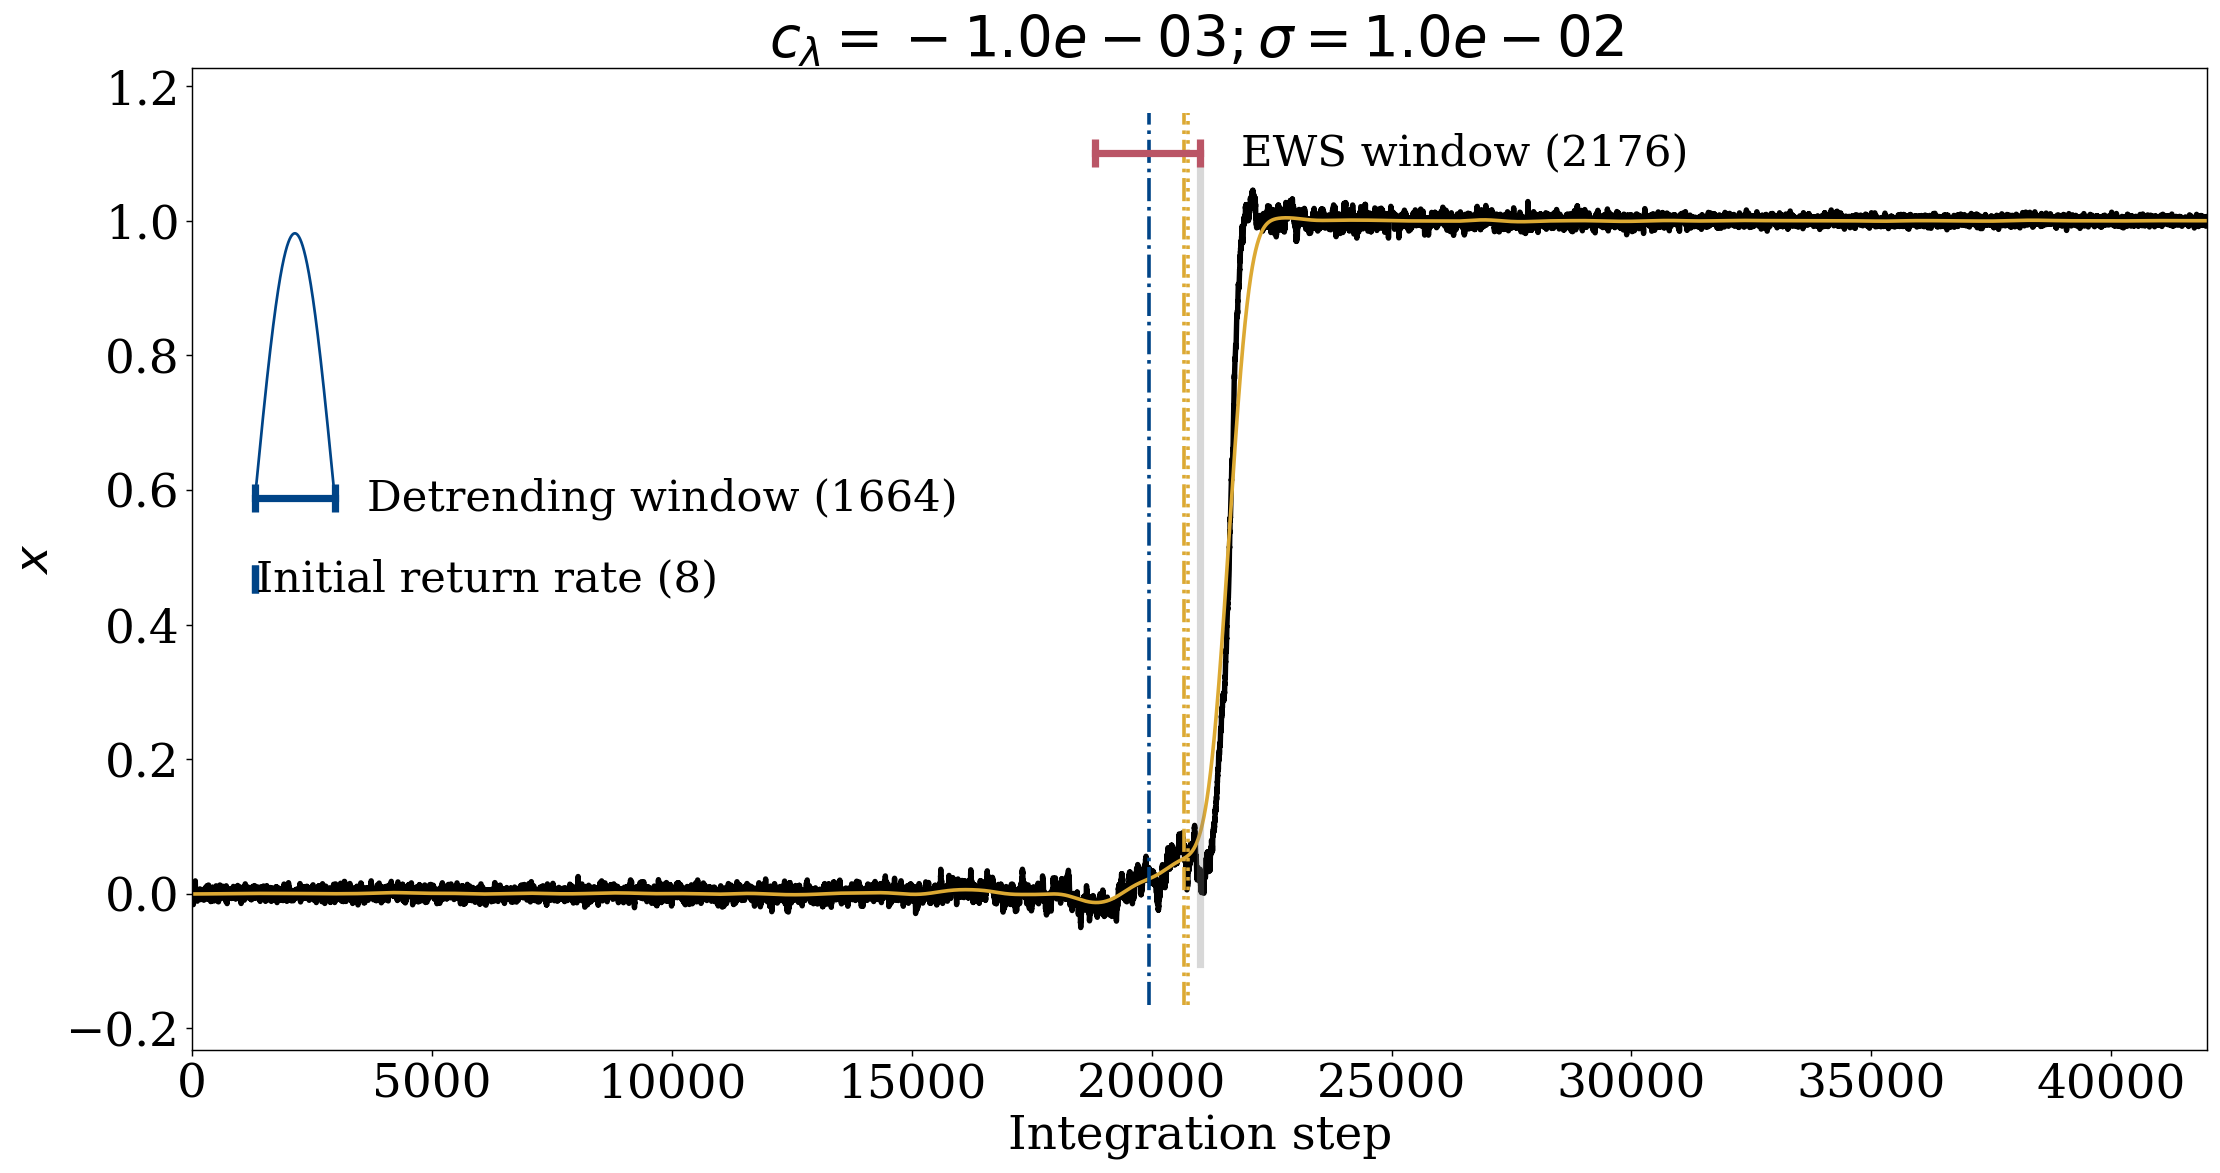
\includegraphics[width=0.8\linewidth]{Images/Metrics/custom_bifurcation/detrend_additive}
	\caption{}
	\label{fig:detrendadditive}
\end{figure}

\begin{figure}
	\centering
	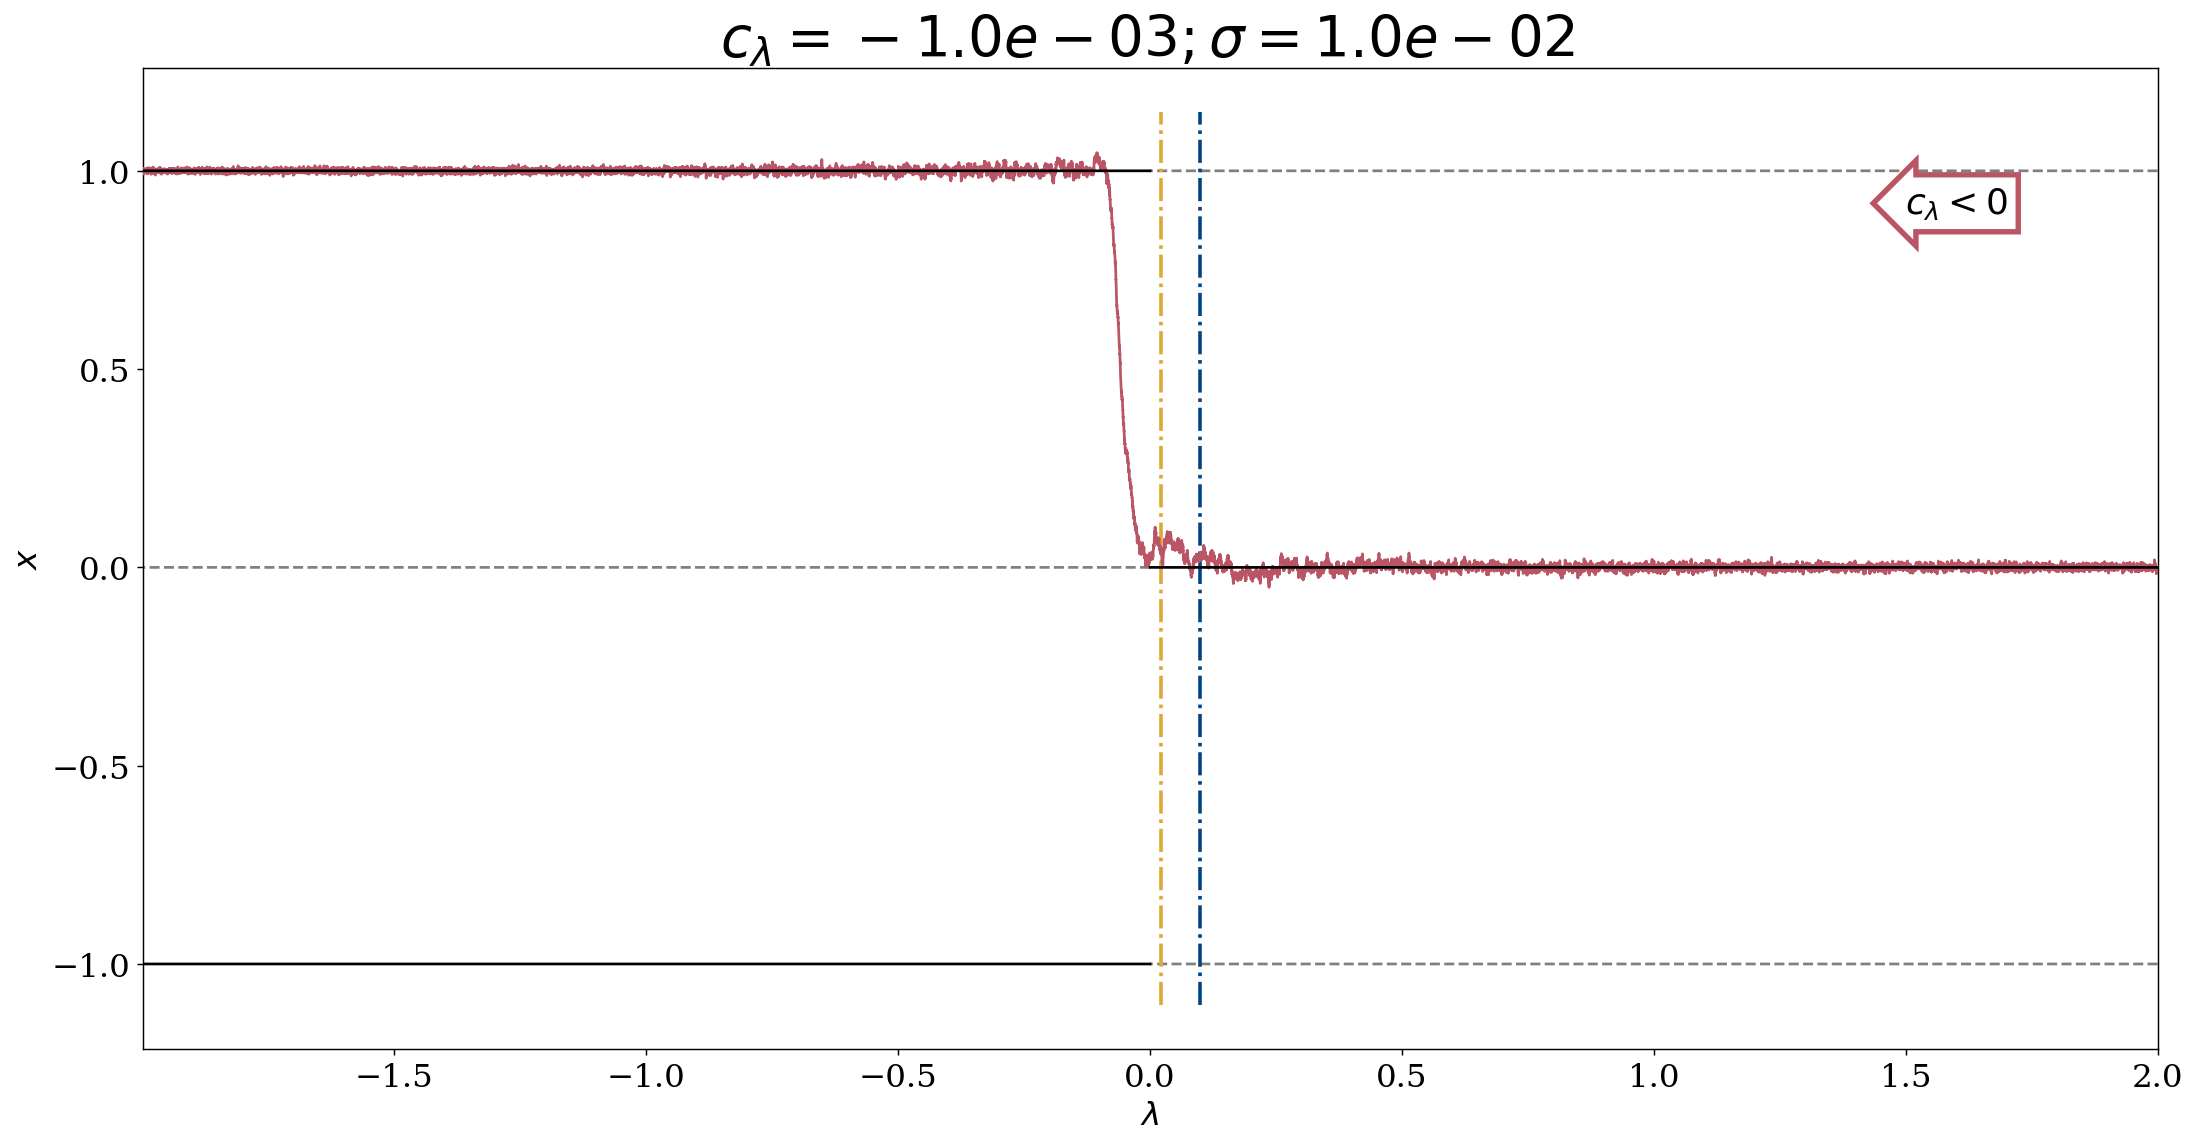
\includegraphics[width=0.8\linewidth]{Images/Metrics/custom_bifurcation/bifurcation_additive}
	\caption{}
	\label{fig:bifurcationadditive}
\end{figure}


\begin{figure}
	\centering
	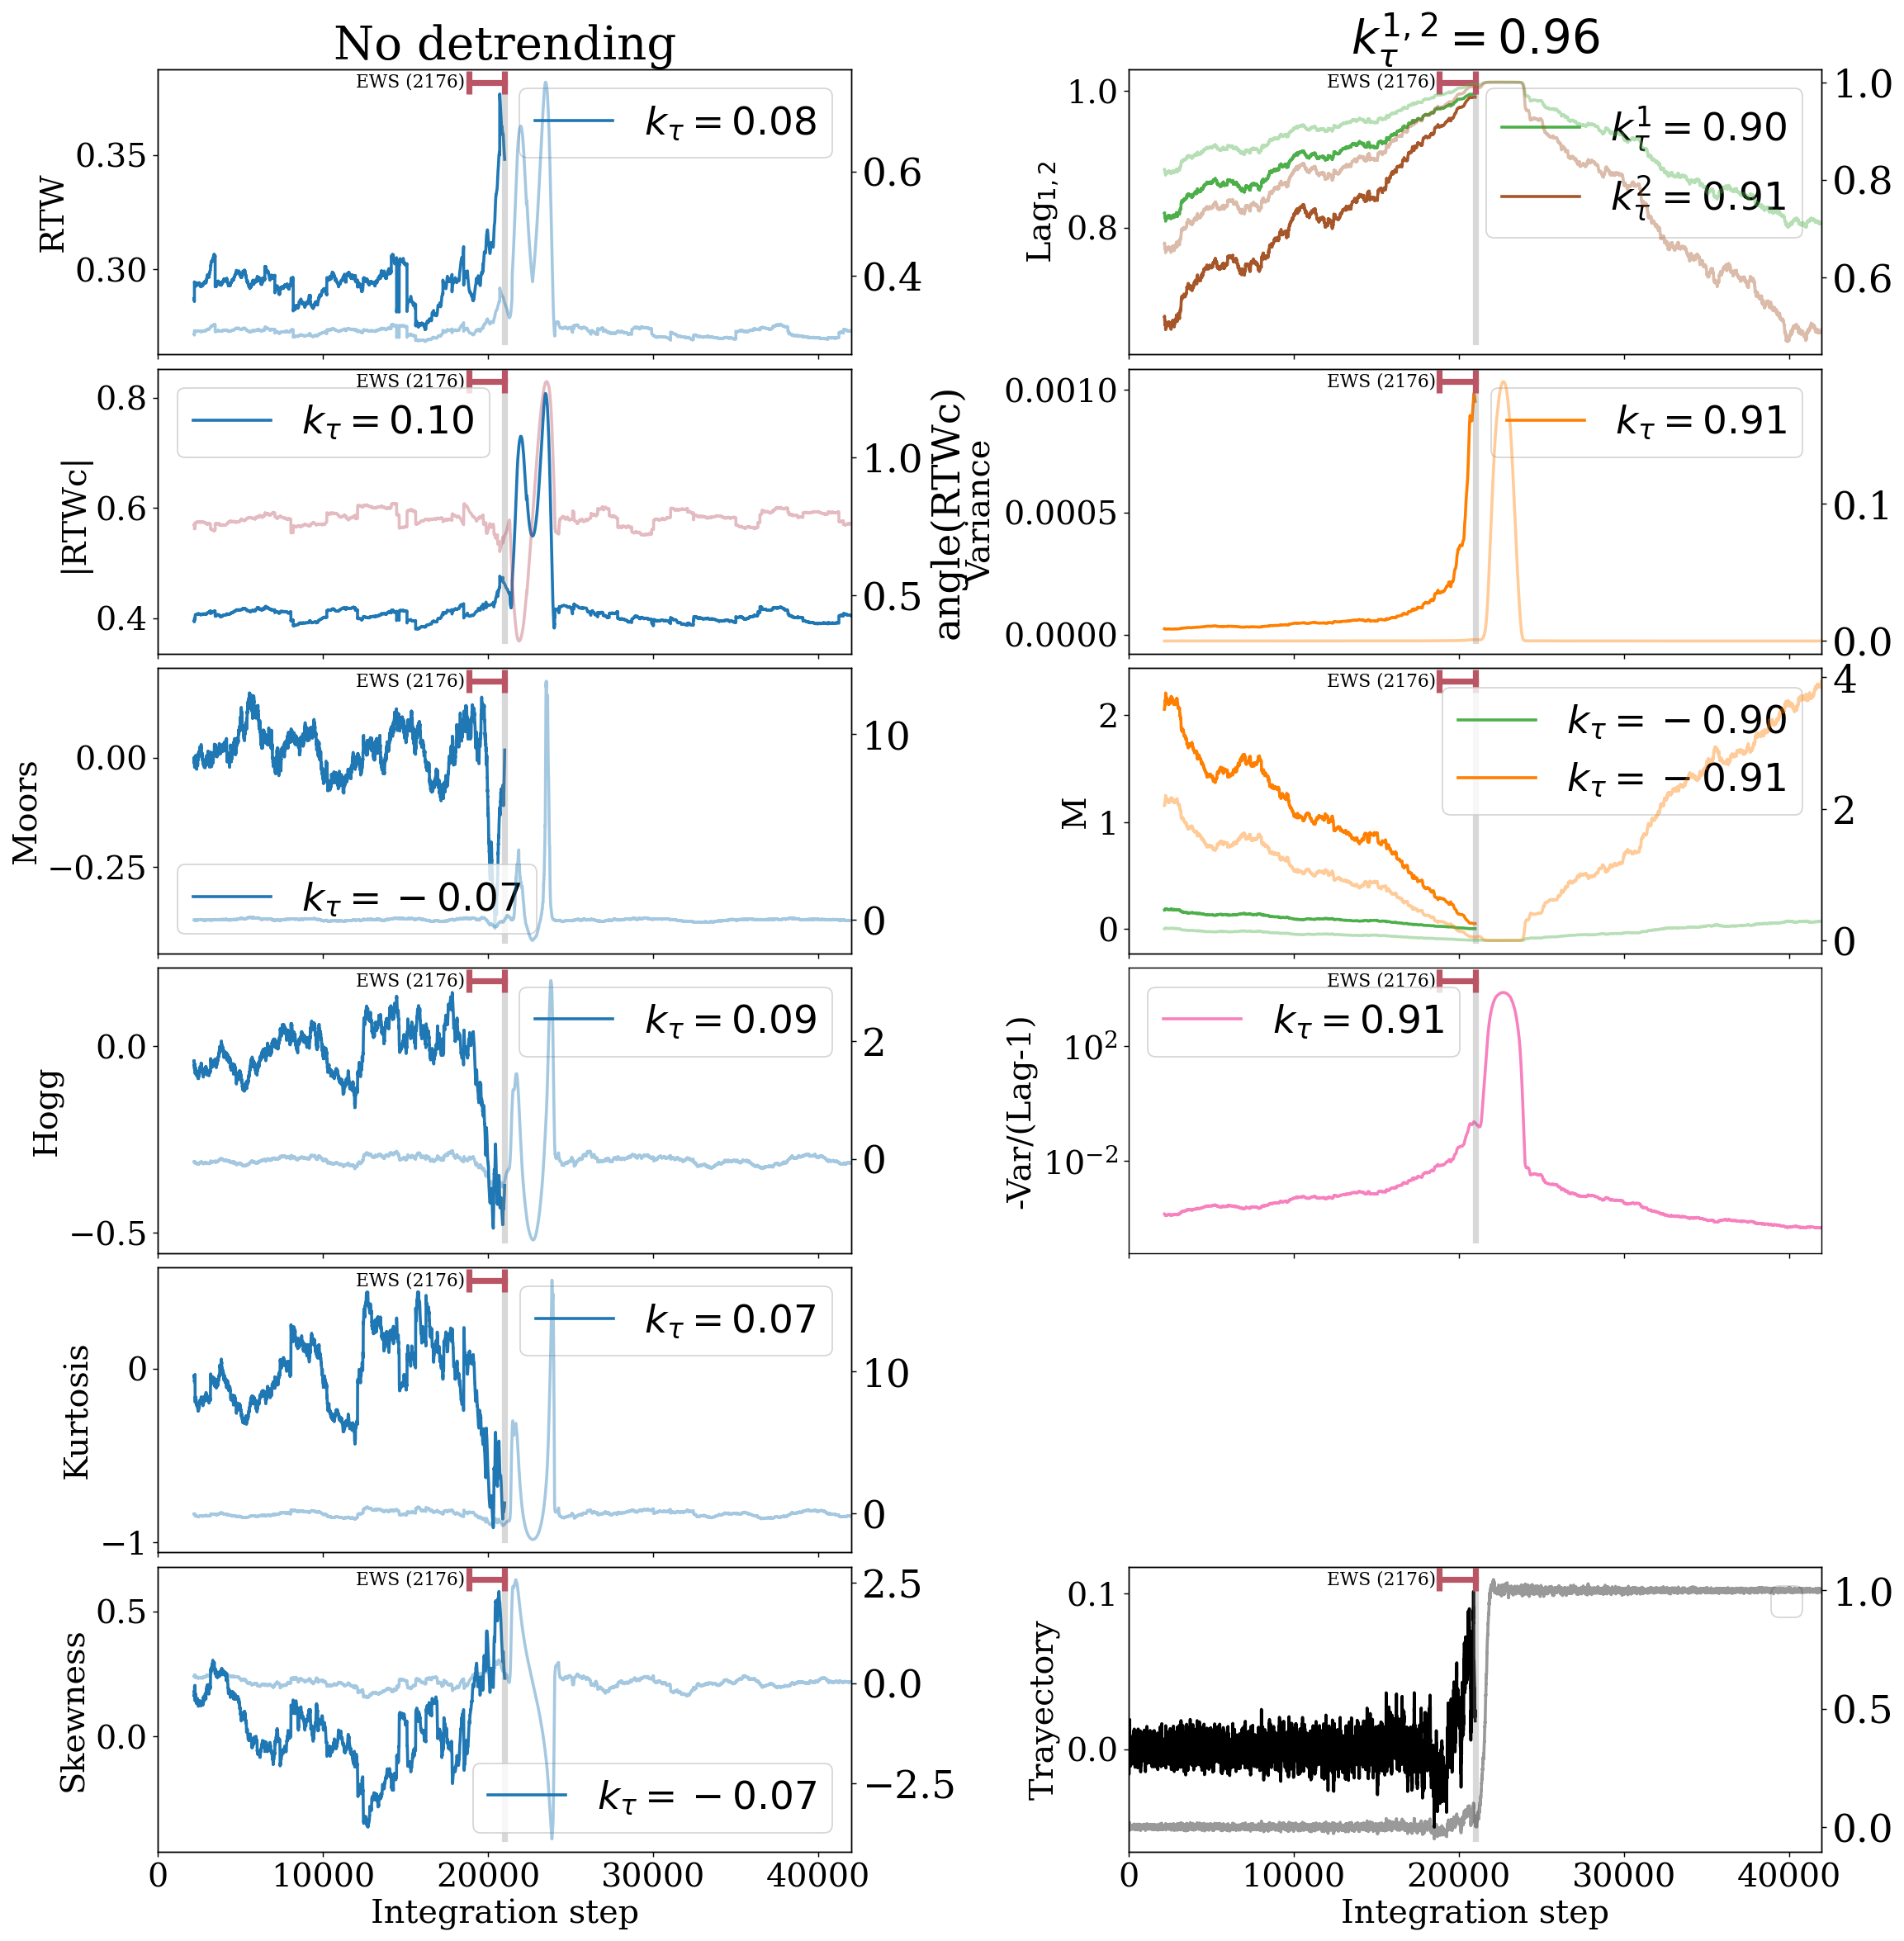
\includegraphics[width=0.8\linewidth]{Images/Metrics/custom_bifurcation/No_det_additive}
	\caption{}
	\label{fig:nodetadditive}
\end{figure}
\begin{figure}
	\centering
	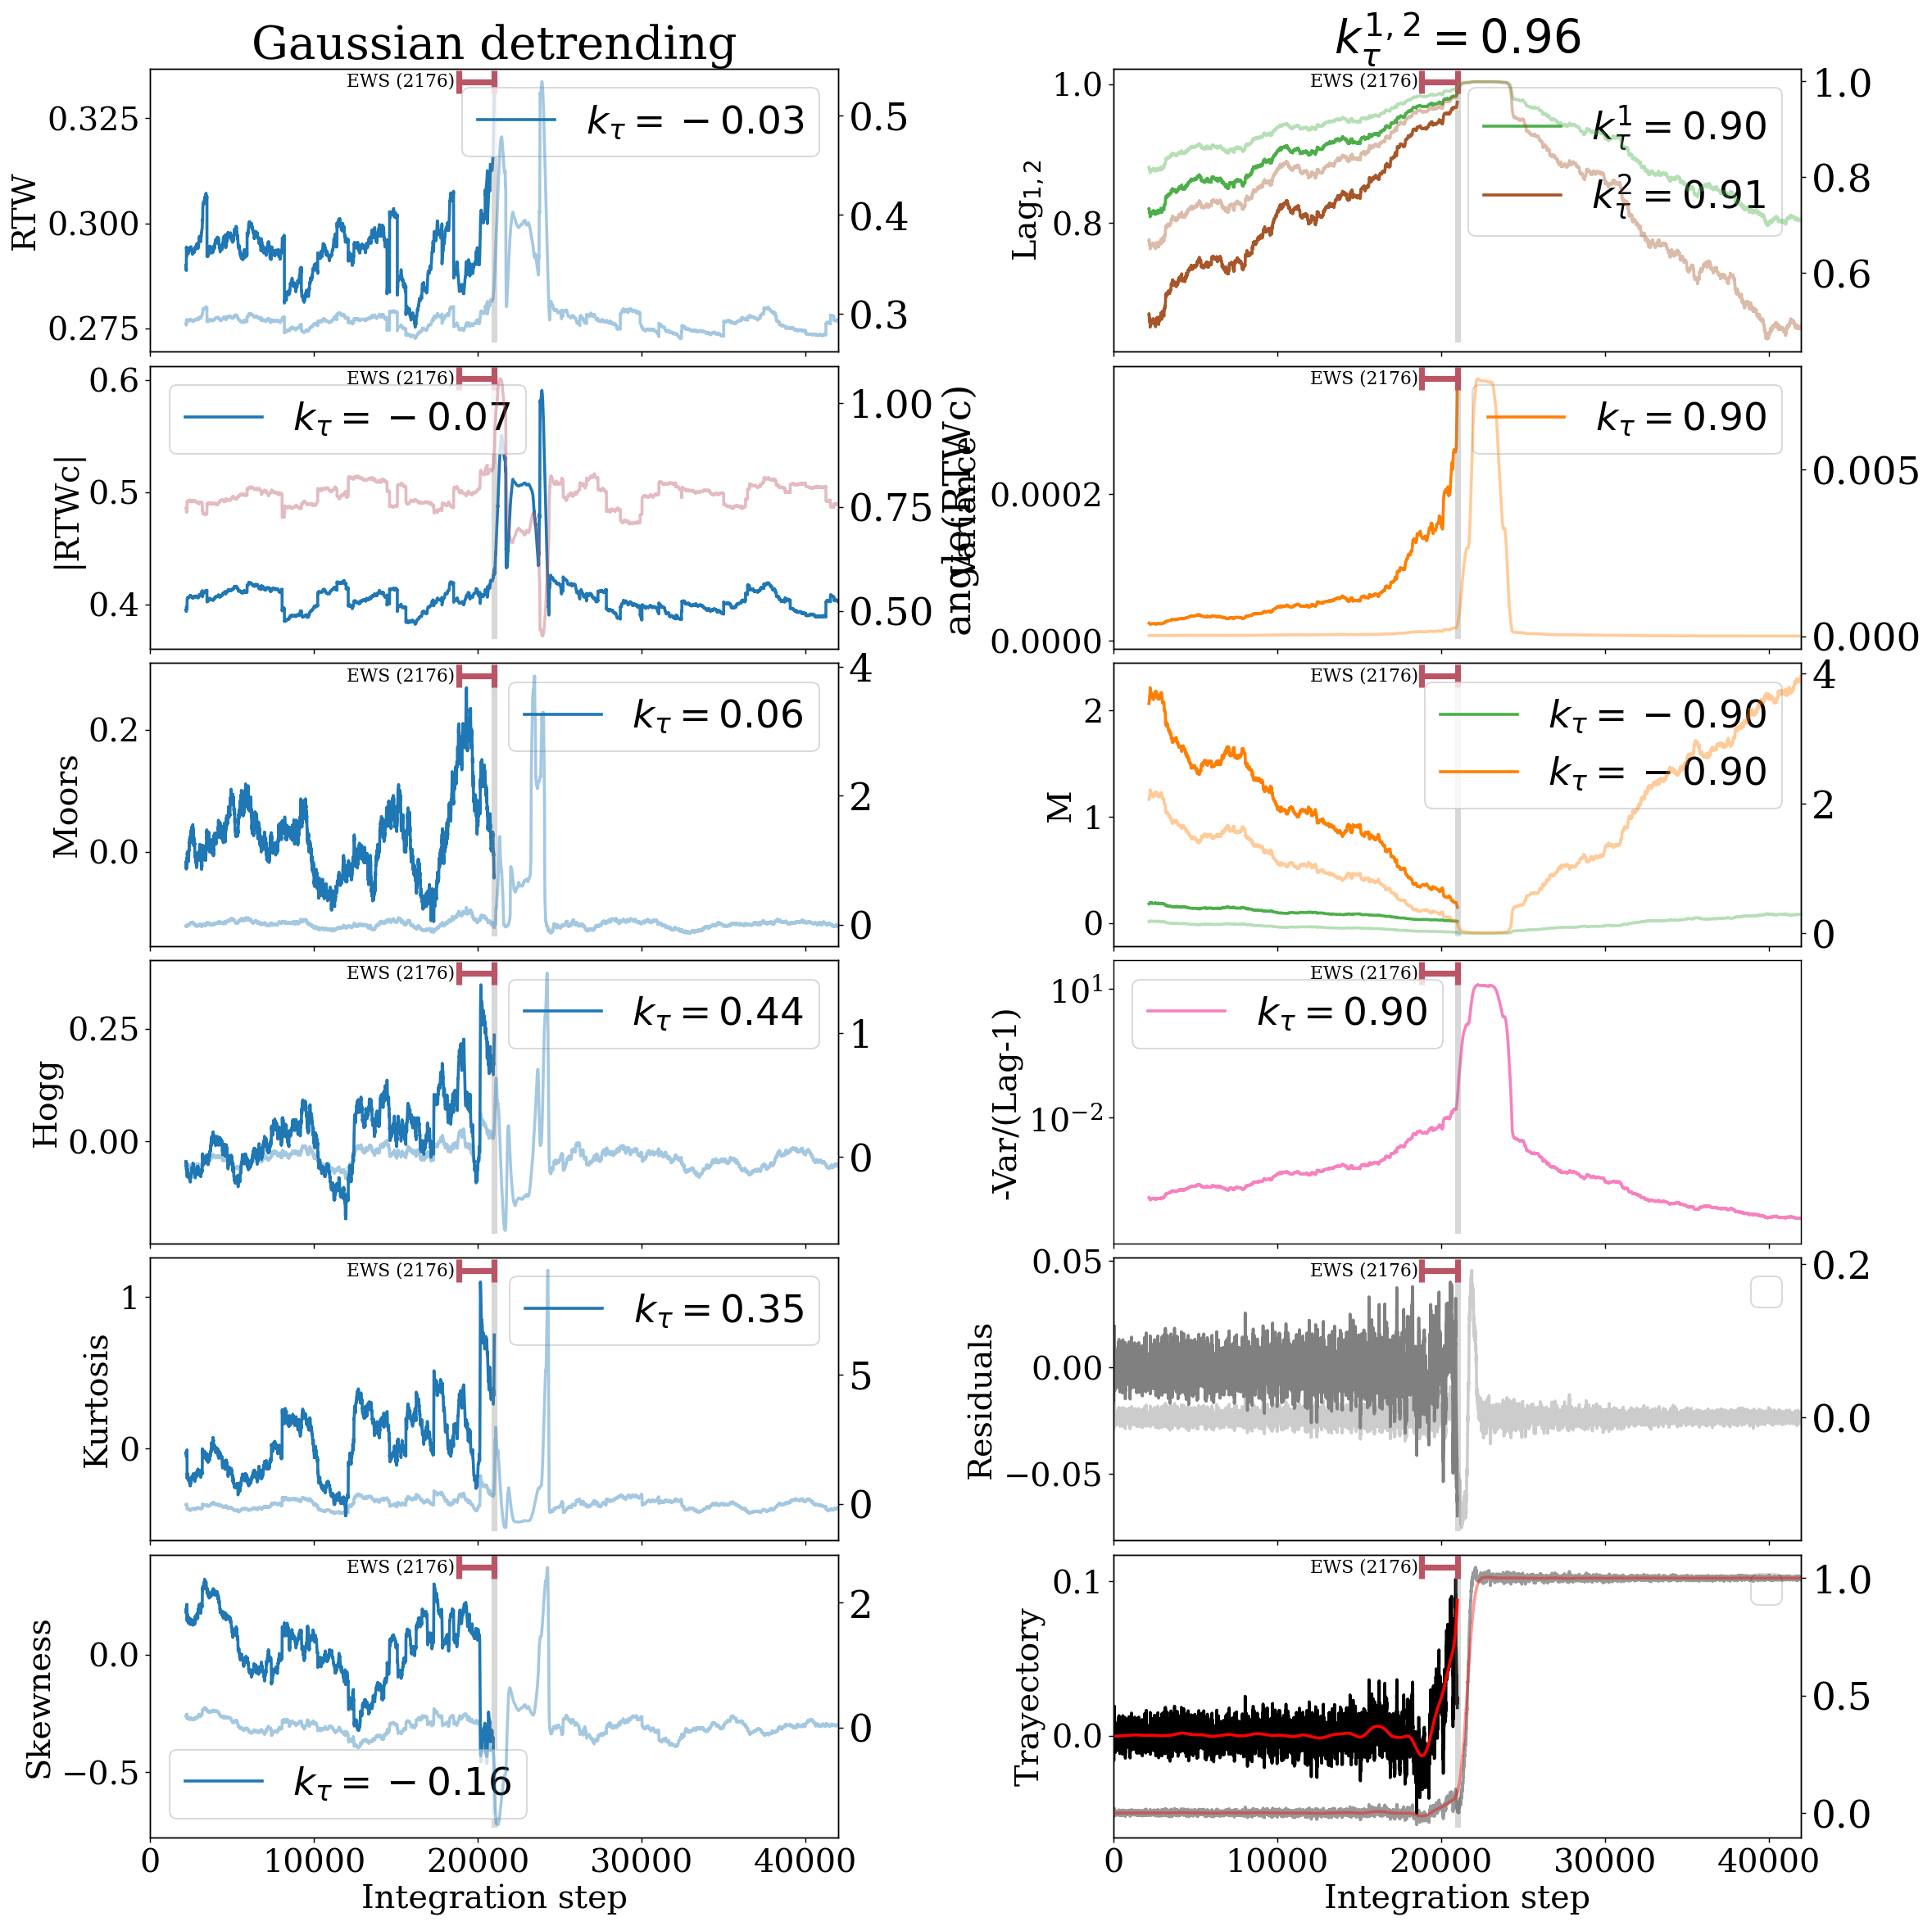
\includegraphics[width=0.8\linewidth]{Images/Metrics/custom_bifurcation/Gdet_additive}
	\caption{}
	\label{fig:gdetadditive}
\end{figure}





\subsection{Sub-critical pitchfork}



\begin{equation}
	\begin{cases}
	dx&=(\lambda x+x^3-x^5) \, dt +\sigma \, dW\\
		d\la&=c_\la \, dt
	\end{cases}
	\label{eq:ASSsubcri_pitch}
\end{equation}



\subsection{Super-critical pitchfork}

\begin{equation}
	\begin{cases}
		dx&=(\lambda x+x^3) \, dt +\sigma \, dW\\
		d\la&=c_\la \, dt
	\end{cases}
	\label{eq:ASSsupercri_pitch}
\end{equation}

This system has three fixed points, $x={0,\pm \sqrt{1/2}\sqrt{1\pm\sqrt{1+4\lambda }}}$



\subsection{Abundance}
	$b=1$,$r=1$
\begin{equation}
	\begin{cases}
		dN&=(rN(1-N/K)-\la \frac{N^2}{N^2+b^2}) dt +\sigma \, dW\\
		d\la&=c_\la \, dt
	\end{cases}
	\label{eq:ASSabun}
\end{equation}

\subsection{Hopf  bifurcation}

\begin{equation}
	\begin{cases}
		dN&=(rN(1-N/\la)-a \frac{N P}{N+b}) dt +\sigma_1  \, dW\\
		dP&=\frac{eaNP}{(b+N)-dP} dt +\sigma_2  \, dW\\
		d\la&=c_\la \, dt
	\end{cases}
	\label{eq:ASSabun_hopf}
\end{equation}



\begin{equation}
	\begin{cases}
		dx&=(\la (x-\la)+(x-\la)^3-(x-\la)^5)dt +\sigma \, dW\\
		d\la&=c_\la \, dt
	\end{cases}
	\label{eq:ASSslanted}
\end{equation}


\subsection{Fold bifurcation}


\begin{equation}
	\begin{cases}
		dx&=(-x^2+cx+\la) dt +\sigma  \, dW\\
		d\la&=c_\la \, dt
	\end{cases}
	\label{eq:ASSfold}
\end{equation}

\subsection{Sharp transition (1) }

In this case, since there is no critical transition, we can choose to be 'slow' though the whole evolution, the only important variable is the separation between the time scale of the control parameter and the timescale of the LDR.
 
\begin{equation}
	\begin{cases}
	dx&=-(x-\mathrm{erf}(10\lambda)) \, dt +\sigma \, dW\\
	d\la&=c_\la \, dt
\end{cases}
\end{equation}



\begin{figure}
	\centering
	\includegraphics[width=0.7\linewidth]{"Images/Metrics/sharp transition/bifurcation_additive"}
	\caption{}
	\label{fig:bifurcationadditive}
\end{figure}
\begin{figure}
	\centering
	\includegraphics[width=0.7\linewidth]{"Images/Metrics/sharp transition/detrend_additive"}
	\caption{}
	\label{fig:detrendadditive}
\end{figure}
\begin{figure}
	\centering
	\includegraphics[width=0.7\linewidth]{"Images/Metrics/sharp transition/Gdet_additive"}
	\caption{}
	\label{fig:gdetadditive}
\end{figure}
\begin{figure}
	\centering
	\includegraphics[width=0.7\linewidth]{"Images/Metrics/sharp transition/No_det_additive"}
	\caption{}
	\label{fig:nodetadditive}
\end{figure}

sharp 2
%r*x[0]*(1-x[0]/K)-l*x[0]*2/(b**2+x[0]**2)
\section{Conclusions}


\begin{itemize}
	\item Skewness as a measure of assimetry already explined by \citep{Guttal2008}

	
	
\end{itemize}
\section{Outlook and remaining questions}

\begin{itemize}
	\item Along this chapter the noise has always been 'forcing' the observable. However, it seem plausible that in many systems, the noise is either present at the same time in the control parameter, or is only present in the control parameter. 
	Otherwise it seems like the noise is only present due to the measuring, or due to some internal hidden mechanism, instead on having a well defined mechanics for the behavior of the system and having a control parameter with an internal variability. 
	For example, measurement from laser intensity can be noisy because of environmental noise, but also because the energy source has variability. 
	In a climate dynamic that is controlled by the temperature, or the solar constant in the case of energy balance model, the noise can be due to internal dynamics, but in can also stem from the internal dynamics of the control parameter (Solar dynamics, local temperature fluctuations, etc.. )
	
	At the time of writing it is not clear if this can have any important effect, but we expect that white noise in a control parameter might present itself as colored noise in the observable (as there is a nonlinear dependence), which can have implications for EWS signals \citep{Dutta2018,Bury2020}, and it might be relevant when considering theoretical developments as the control is not longer a fully deterministic variable. 
	
	This can also have influence in the capacity of having earlier warning as the noise on the control parameter would allow the system to 'tip its toes' into the tipping, while not being (on average) at the tipping point, possibly allowing for earlier warnings.
	
	As shown by \cite{Patterson2021} the directionality, and how the noise is presented in each parameter has great implications for the  the quality of the EWS, even when the noise is directly applied to the dynamical variables.
	
	which brings us to the next open question:
	
	\item What is the extension for our adiabatic definition for higher dimensional systems? This is specially interesting for R-tipping since there, the effect depends on having well defined the speed of the forcing parameter. 
	In this case the adiabatic definition will also have directionality as in \cite{Patterson2021}.
	
	So far the deductions for sweeped systems that we have found assume some adiabatic/ergodic behavior in their deduction. As example,  \cite{Romano2018} has a mathematical deduction for a 1-dimensional ASS system and the goodness of EWS, however they also assume the sweeping rate to be small enough to consider adiabatic behavior. 
	
	\item Many works have been developed for either additive or multiplicative noise and how this might effect the EWS, to our knowledge there is no work in systems with several sources of noise, for example a systems that evolves with an underlying white noise, but also with stochastic shocks present, and how this shocks might modify the EWS signals.
	
	\item Questions for Lucarini (or others): Using kurtosis or other metrics instead .  R-tipping and van der pol oscillator.
	
	\item 
	Since the relaxation time changes through the evolution, it would be numerically cheaper to not have an evenly spaced signal, but to change the resolution of time according to the relaxation time.

	\item Prove that some EWS in stochastic systems with a changing parameter do not work  when the pullback attractor does not follow the stable path.   
	
	Rate-Induced Tipping in Discrete-Time Dynamical Systems-Claire Kiers
	

	

	\item Does overshooting a bifurcation like and returning quick as in \cite{Ritchie2021} still work in higher dimensions?. In 1D this might work since the system is forced to come back due to the forward stability when returning the control parameter, however in higher dimensions the system might prefer to avoid crossing the unstable branch through another path.
	
	\item Is there an effective return time near a bifurcation? how can it be estimated?

	
	
	\item Variance might change without getting close to the bifurcation, and it is also not bounded nor has a steady state. 
	
	\item cluster machine learning and topological things. \cite{Gidea2020}
	
	\item kurtosis,skew,kr,etc.. might be better for a slow moving variable since there is an equilibrium better defined
			
	\item Skewnes/kurtosis in the ornstein picture are related to ghosting.
		
	\item To optimize the signal quality of the EWS, it could be possible to develop a sliding window that changes depending on an estimate of the lag-1.  Since the correlation time changes, the moving windows width and bandwidth should also change to have better statistics.
	
	\item 	There is something better than bootstrapping? I understand it's supposed to be 'sub-optimal' for biased statistics like kurtosis, there are ways to implement saddle point or edgeworth approximations that would work better?
	
	\item It would be useful to develop an automatic estimate of when the bootstrapping is close to reproducing a normal distribution since different statistics might need different number of bootstraping resamples. 
	An early attempt to develop this using the Pearson coefficient from scipy.stats.normaltest so far has been very slow, which might be due to some moments not converging well enough for reasonable amounts of computation.
	\item I wonder the distribution of time the system spends above or below the mean can be used as indicator. (and the time length distribution for this values.)
	
	
	\item $dx^*/dt=nonlinear non-inertial acceleration.  $
	
	augmented system (in 1d) should be 
	
	\begin{equation}
		\begin{aligned}
			d x&=f(x,\lambda)dt+\sigma dW,\\
			\dot \lambda&= c_\lambda >0.
		\end{aligned}
	\end{equation}
	
	which in our case
	\begin{equation}
		\begin{aligned}
			d x&=[f(x,\lambda)- \frac{d x^*}{dt } ]dt+\sigma dW,\\
		\end{aligned}
	\end{equation}
	
	
	\item Complex, continous 1D equations as stand in for discrete systems?
	
	\item Null bandwith\cite{Kaur2022}.
	\item what happens when adding noise to the forcing. since i suspect this might be the most common case.
	\item Develop an ROC (receiver-operating characteristics) method to judge the metrics similar to what was done by \cite{Bury2020,Romano2018}. Alternatively it could be possible to do a test like the one done by \cite{Kaur2022} where they shown violin plots for the Kendal-$\tau$ values over several realization of their case studies.
		
		\item 
		for the detrending for the CSD low moments metrics it makes sense to use an average based detrending since we want to recover OU based results. However it might be better to use other detrending approaches for studies with higher moments related to the tails of the data. Like the detrending used in \cite{}.
\end{itemize}
\section{List of symbols}

\begin{tabular}{ l c}
	$\lambda$ & Parameter that can be swiped \\
	$ f(x,\lambda) $ & Deterministic backbone \\
	$x^*(\lambda)$  & Equilibrium of the deterministic backbone \\
	$M=\frac{D f}{D x}(x^*)$  & Jacobian matrix of the deterministic backbone, at a given equilibrium. \\
	$m$  & Eigenvalue of $M$ \\
	$\sigma$ & White noise intensity of the stochastic process. 
\end{tabular}





\newpage

%\includepdf[pages=-]{Papers/PhysRevLett_freezing.pdf}

%\newpage

%\input{Chapters/Rogue_waves_adiabatic}
%\input{Chapters/Rogue_waves_adiabatic_body.tex}
%\newpage
%\includepdf[pages=-]{Papers/Armaroli2020_Article_StabilizationOfUni-directional.pdf}
%\newpage

	\clearpage
	\begin{appendices}
		

\chapter{EWS appendix}

\subsection{Rogue events index}	
A simple way to compare tailedness of distribution in a frequentist manner, would be to count the amount of Extreme Events (EE), since these are defined as rare events and therefore always reside in the tails. 
There are several definitions of EE in different fields.

In the ocean community they are called Rogue Waves (RW) and are defined as any event higher than two times the significant wave height ($H_s$), which is defined as $H_s=U_{1/3}$. 
Using this definition we can count the amount of these events in our series and compare with the expected amount and this would give us an idea of how the tails behave. 

Since for a Rayleigh distribution\footnote{The Rayleigh distribution is the expected distribution for a linear superposition of waves with a narrow banded spectrum and low steepness.} it is expected to see one extreme event every 2980 events, we can define 

\begin{equation}
	RR1=\frac{(\textrm{\# events}>2U_{1/3})\times 2980}{\textrm{\# events}}
	\label{defRR1}
\end{equation}

With this definition, a Rayleigh distribution has $RR1=1$. Distributions with $RR1 >1$ have 'higher' tails than a Rayleigh distribution. 

In the same way, other metrics analogous to the previous one can be constructed to compare with other distributions, for example an exponential distribution \footnote{In optics, the expected distribution from narrow banded pulses in the linear regime is an exponential. } has 45 extreme events every 3000 events, thus 
\begin{equation}
	RR1_{exp} \approx  \frac{RR1}{45}
	\label{defRR2}
\end{equation}
With this definition, an exponential distribution has $RR1_{exp}=1$.

As defined, these methods of counting EE as a way to characterize the tail have a main problem: any metric defined only with respect to $U_{j}$ is not independent from translations.

For our applications, just like we did for the Pareto metric in eq.~(\ref{eq:pareto_offset}), to make sense of this as a shape metric we need to make it translational invariant. 
So, before evaluating the data, we offset the distribution with its lowest value, in such a way that it is always positive and starting from zero 
\footnote{while I do this to be able to compare offset data, it's also true that the original definition gives more sense to an 'Extreme'.}.

It should be noted that some works in the ocean wave community, and even in the optics community \citep{Alexis1,...,..}, use different definitions for $H_s$, like  $H_s=2\sigma $(where $\sigma$ is the variance of the Gaussian distribution \footnote{of the surface elevations} related to the Rayleigh distribution \footnote{for the envelopes} \citep{Onorato2011}) or $H_s=2.2~std(H) $.
These definitions are equivalent to the original one only for a Rayleigh distribution and thus we will not take them into account. 

%The rogue events index \ag{[REF?]} is a more direct determination of the %rogueness or tailedness of a distribution. Following XXXX \ag{[REF]}, we %consider rogue events as events with a magnitude exceeding $4\sigma$ %deviation from the sample average, in either direction \ag{[Correct? Did %you use this definition, or the 2.2 standard wave height?]}. The index is %the ratio the number of such events to the total number of events.

In this sense we could, for example, use the same idea to define another Rogue wave index using other definitions of $H_s$\footnote{Maybe i should add this to the supplementary}.

%	\subsection{Rogue wave comparison}
%	
%	Lastly, the most trivial way to compare if a distribution has more or less extreme events than another could be to compare with a known case. 
%	For example, under the definitions of extreme events, for the Rayleigh distribution, the probability of an event exceeding the threshold of two times the average of the highest third of the distribution is 1/3000. 
%	So, the same definition of extreme event can be used on another distribution and we can just compare the probabilities of exceedence. 
%	
%	The problem with this definition is that it depends both on the definition of extreme event threshold, and on the distribution to be compared. 
%	But, this could also be an advantage, since in some cases it is known how the distribution should look if the hypothesis of an underling normal distribution where true. 
%	
%	For example, for a normally distributed electric field, the intensity should follow an exponential distribution\cite{intensity}, thus it would be natural to compare against this. 
%		




\section{Pitchfork toy model}

This toy model is based on the well known pitchfork bifurcation \mb{with normal form} given by

\begin{equation}
	\dot{y}=r y-y^3
	\label{eq:pitchfork}
\end{equation}
This equation displays a bifurcation diagram like the one shown in Fig.~\ref{fig:bifdiag}, where given an initial condition $y_0$, the system goes from having only one stable solution ($y^*=0$) for $r<0$, to having two stable solutions ($y^*=\pm \sqrt{r}$) separated by an unstable branch for $r>0$.
\begin{figure}[htb]
	\centering
	\begin{tikzpicture}
		%	\tzaxes(-0.5,-2)(2,2){$x$}{$r$}
		\tzfn[black,thick]{sqrt(\x)}[0:2]{}[ar]	
		\tzfn[black,thick]{-sqrt(\x)}[0:2]{}[ar]	
		\draw [-,thick](-2,0) -- (0,0);
		\draw [dashed,thick](0,0) -- (2,0);
		\draw [->,thin,opacity=0.4](-2,0) -- (2.5,0)  node[right] {$r$};
		\draw [->,thin,opacity=0.4](0,-1.4) -- (0,1.4) node[above] {$x^*$} ;
	\end{tikzpicture}
	\caption{ Pitchfork Bifurcation diagram; $y^*$ is the value of $f$ after some time $t^*$. $r$ is the bifurcation parameter.}        
	\label{fig:bifdiag}
\end{figure}



Now, let us consider a normal distribution of initial conditions $y_{0j}$. By keeping $r>0$ and varying the mean of the distribution and its variance, we control how likely it is for a given initial condition to be in the basin of each stable branch in Fig.~(\ref{fig:bifdiag}). In this way the amount of solutions in each basin switches and this can lead to extreme events when the set of initial conditions is near the unstable branch ($<\! y_{0}\!>=0$).

In order to obtain a switch, it is also necessary to introduce some noise on the parameter $r$. In this work we choose to consider Gaussian noise of variance $\Delta r$.
This means that the solutions near the stable branches after some large integration time will have a broader and almost Gaussian distribution related to $\Delta r$. 

\begin{figure}[H]
	\centering
	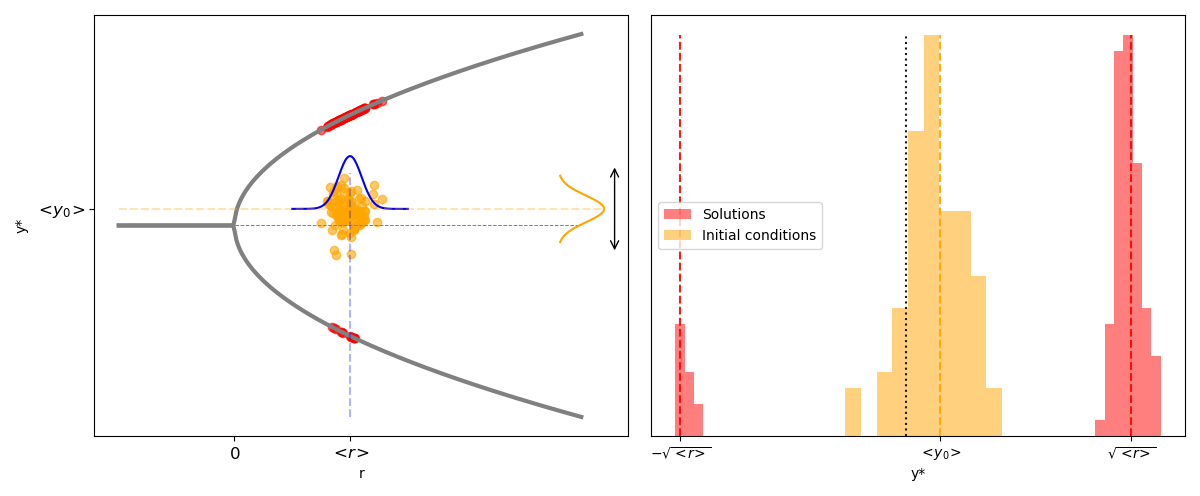
\includegraphics[width=\linewidth]{Images/Metrics/pitchfork_explanation.png}
	\caption{Scheme of the pitchfork transition. The stable branches of the bifurcation diagram are shown in gray solid line. A set of initial conditions with Normal distribution with mean value $<y_0>$ is in orange. Each of these initial conditions is then integrated for a given time $t^*$ for a random parameter $r$ obtained from sampling a normal distribution of mean $<\!r\!>$ and variance $\Delta r$. 
		The results of this integration gives the set of final solutions shown in red. 
		By moving $<\!y_0\!>$ between the stable branches, we obtain transition statistics of the set of solutions for each $<\!y_0\!>$.}
	\label{fig:pitch-explanation}
\end{figure}

At each realization, the parameter $r$ and the initial condition $y_0$ are chosen randomly as stated before, and after some integration time $t^*$ (the same for all realizations) the value $y^*$ is saved. 

In this case, the tails of the distributions when approaching the transition are controlled by the integration time $t^*$ due to critical slowing down. 

\begin{figure}[H]
	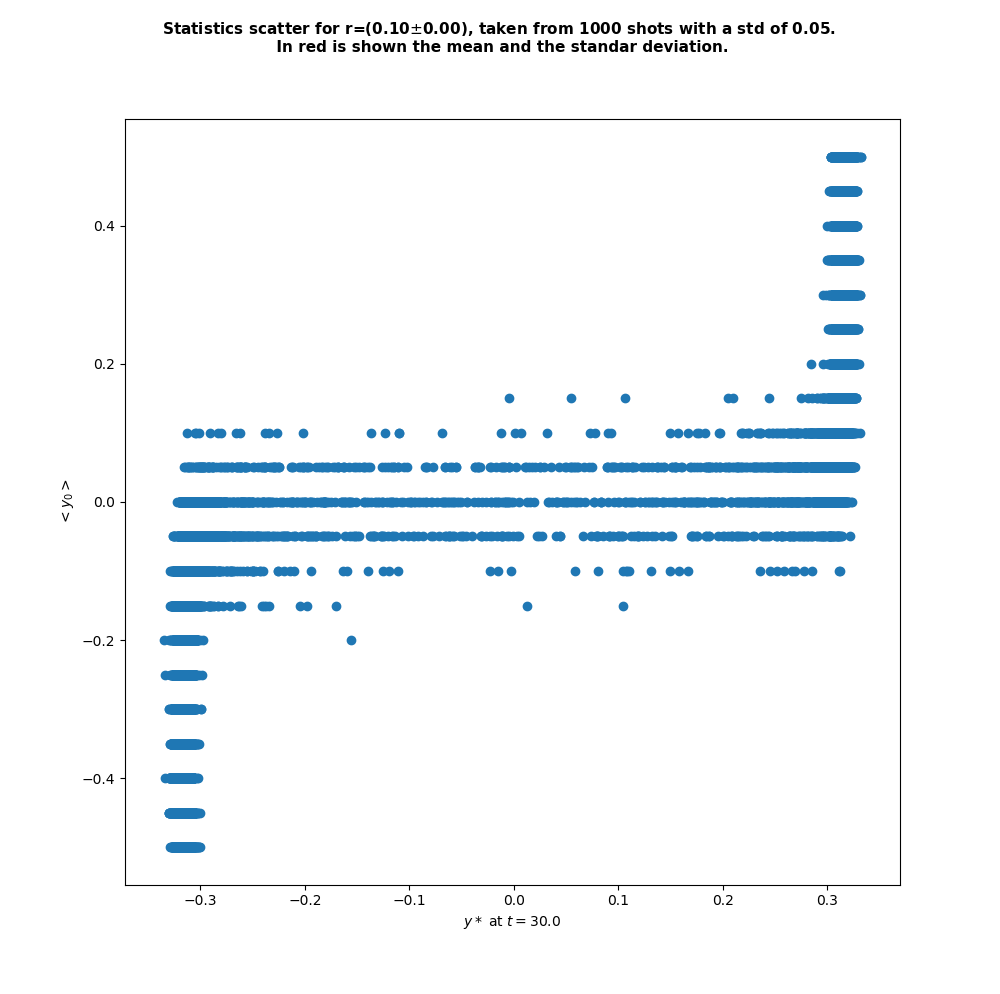
\includegraphics[width=0.3\linewidth]{Images/Metrics/t_30.png}
	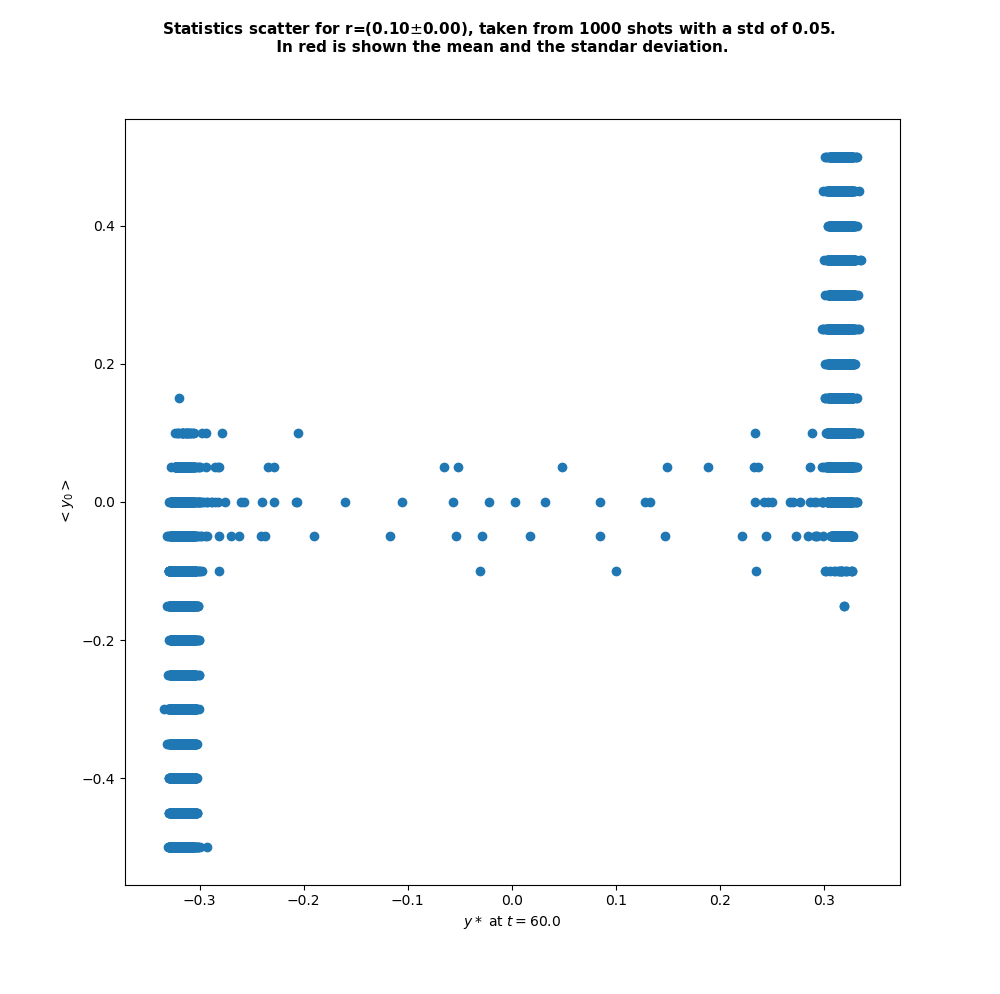
\includegraphics[width=0.3\linewidth]{Images/Metrics/t_60.png}
	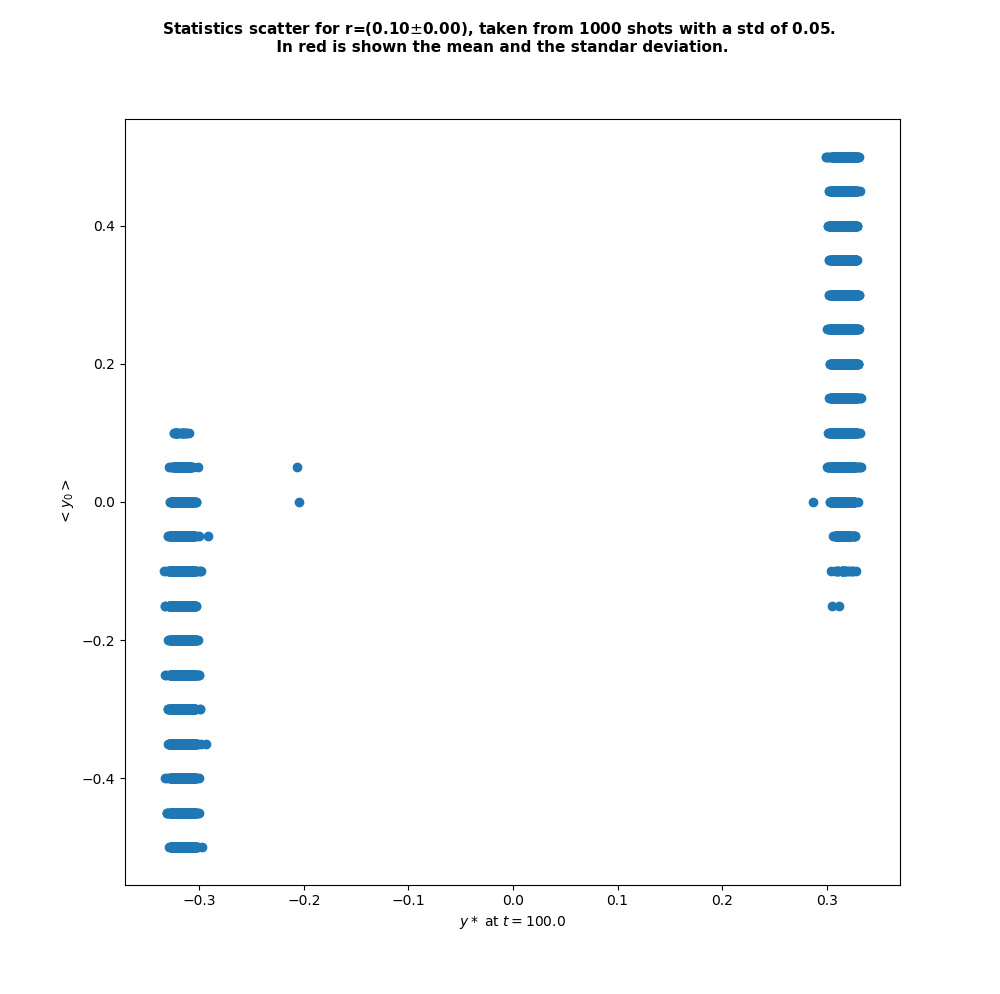
\includegraphics[width=0.3\linewidth]{Images/Metrics/t_100.png}
	\caption{Effect of the integration time on the statistic. The integration times are $t=30, 60, 100$. All other parameters remain constant.}
	\label{fig:critical_slowing}
\end{figure}

This means that the closer the system is to the bifurcation, the more time it takes for a given initial condition to approach the steady state. 
Therefore, for a given integration time $t^*$ the closer the system is to the bifurcation, the more likely it is to 'measure' results far from the stable solutions. 

Figure \ref{fig:critical_slowing} shows the resulting scatter plots for different integration times. In these simulations $<r>=0.1$, $\Delta r=0.003$, and the standard deviation of the initial conditions is $\Delta y_0= 0.05 $ with 1000 points taken for each realization.

\mb{Figure 10: comment on this figure} 

\begin{figure}[H]
	\centering
	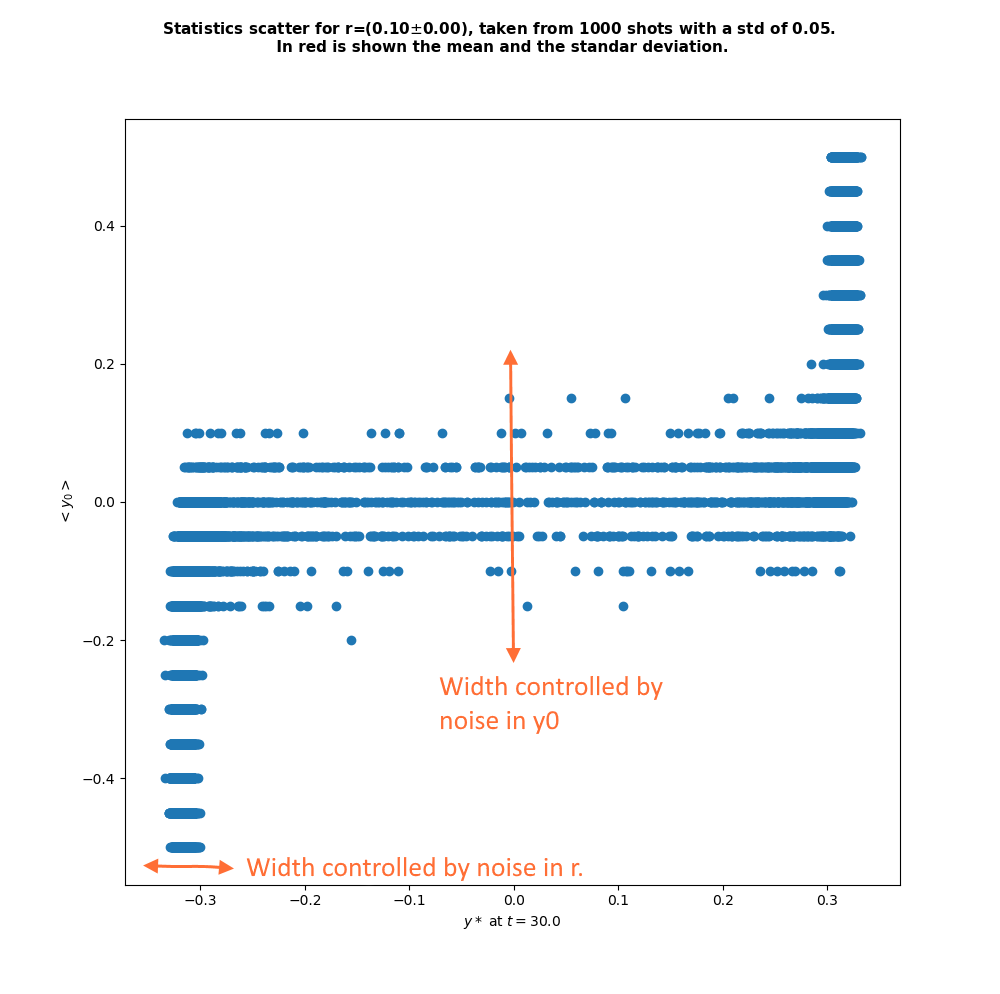
\includegraphics[width=0.4\linewidth]{Images/Metrics/Parameters.png}
	\caption{Effect from critical slowing down.}
	\label{fig:parameters}
\end{figure}
\section{paradox?}



Coming back to the system from eq.~\ref{eq: simplecase}; we can exchange time and control parameter since $\lambda=c_\lambda t+\lambda_0$,and  $\int_{\lambda_0}^{\lambda(t)} \frac{d\lambda}{\dot \lambda}=\frac{\lambda-\la_0}{c_\lambda}$ so 

\begin{equation}
	\lim_{\lambda\to\lambda_c=0} Var[x]=\frac{\sigma^2}{2 |\lambda|}(1-e^{2\frac{\lambda^2}{c_\lambda}})=\frac{\sigma^2}{2 |\lambda|}(2\frac{\lambda^2}{c_\lambda}-\frac{(2\lambda^2/c_\lambda)^2}{2}+\frac{(2\lambda^2/c_\lambda)^3}{6}-\dots)=0
	\label{eq: ST_wellexample}
\end{equation}
\textcolor{red}{correct this.}

\section{Stochastic adiabatic timescale}
\label{apx:sameinit}


\begin{figure}[htb]
	\centering
	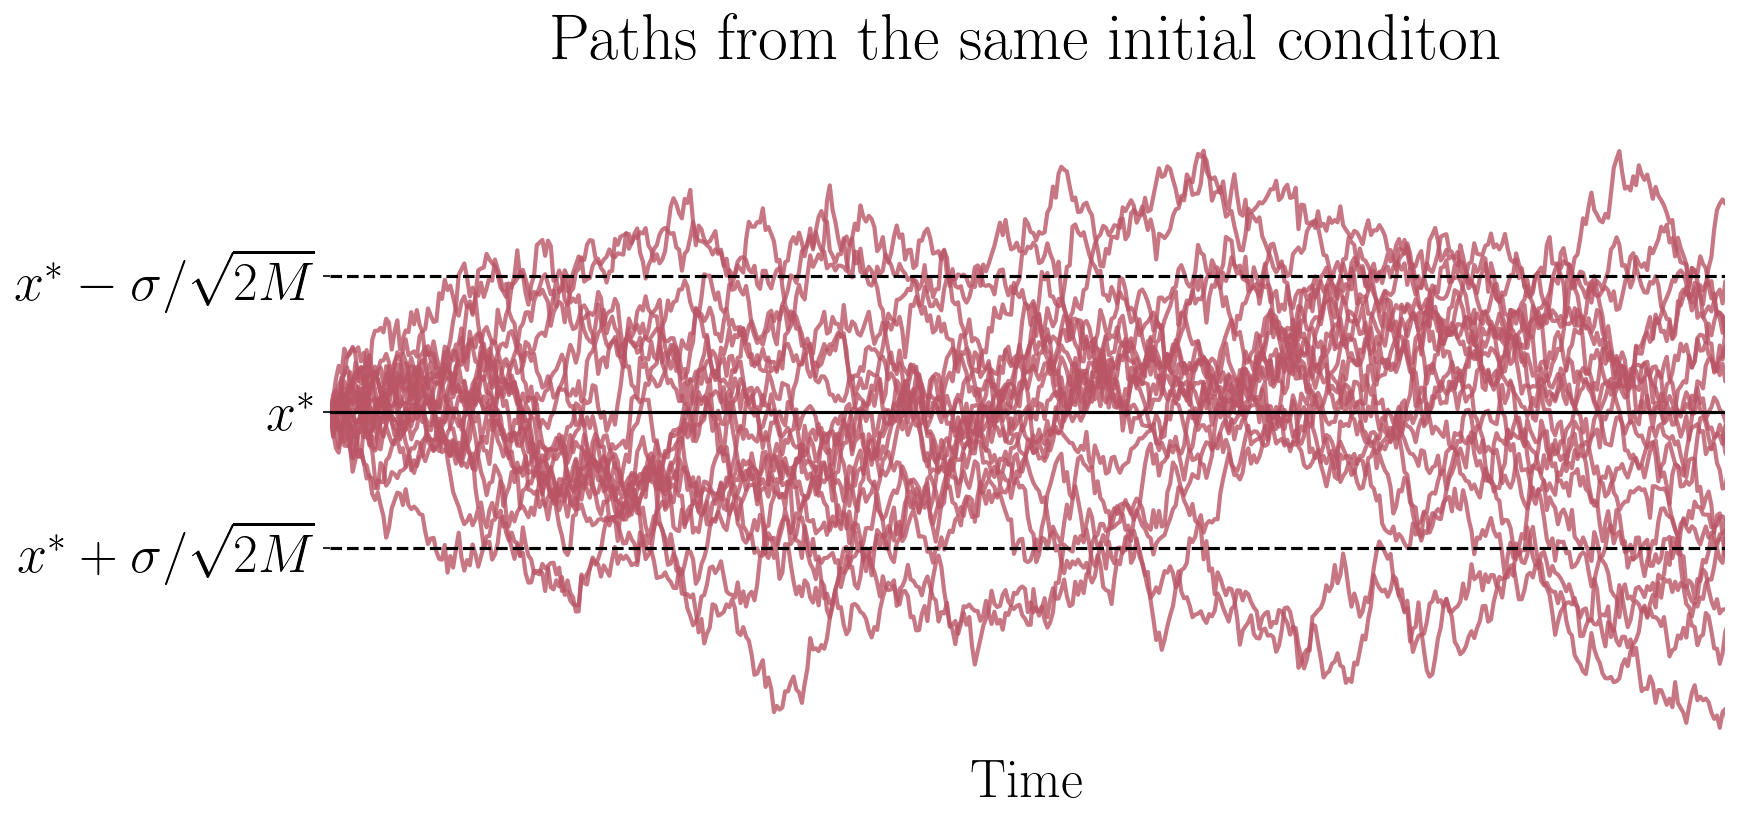
\includegraphics[width=0.9\linewidth]{Images/Metrics/same_init2}
	\caption{20 integrations of}
	\label{fig:sameinit}
\end{figure}



\begin{figure}
	\centering
	\includegraphics[width=0.9\linewidth]{"../Programing Proyects/EE indicators/Simulations with pdfs to test/Stochastic equations/SDE tests jupyter/image_variance_speed/x0_0_tests/toghether/000_variance_test_speed_toghether"}
	\caption{}
	\label{fig:000variancetestspeedtoghether2}
\end{figure}



\begin{figure}
	\centering
	\includegraphics[width=0.9\linewidth]{"../Programing Proyects/EE indicators/Simulations with pdfs to test/Stochastic equations/SDE tests jupyter/image_variance_speed/x0_0_tests/toghether/016_variance_test_speed_toghether"}
	\caption{}
	\label{fig:016variancetestspeedtoghether}
\end{figure}



\section{Extreme events}

Extreme events are unexpected events, both in amplitude and by appearance, compared to the typical dynamics of a system, and might have big consequences. 
By definition,  this events are related to 'heavy tails' on the probability distribution function (PDF) of the systems, that is to say, events that are different to the mean behavior of the system but also rare. 

There are several definitions for extreme events in the literature depending on the subject, but the broad implications and applications they have makes their study interesting. 
This  can range from  extreme events in finance, where they are typically called Black swans or Dragon kings depending on their characteristics \cite{..}, like financial crisis, big fluctuation in the market\cite{bibid}, or bubble bursts\cite{bibid}; to rogue ocean waves that bring down cargo ships \cite{..}, large earthquakes \cite{bibid}, extreme weather\cite{bibid}, population dynamics\cite{bibid}, degree distribution in complex networks\cite{Eom2015}, internet trafic \cite{Hernandez-Campos},  and many more.

Each system can have a different mechanism by which this extreme events are possible, but typically this are due to intrinsic nonlinear responses of the system. 

Some examples of this are self-focusing of ocean waves\cite{..} or laser intensity profiles \cite{..}, large amplitudes due to unlikely explorations of chaotic systems \cite{..}, large fluctuations on systems going through critical transitions \cite{..}.

The study of such events is not only useful for the understanding of their emergence and the feasibility of their forecast. 
But the way a system responds to fluctuations can give us information about some intrinsic properties of a system. 


Given this \textbf{zoo} of behaviors it is clear that a key problem when studying this systems is our capacity to know how they might behave, in particular when they can display big fluctuations or strange or \textbf{freak} behaviors, but also understanding when they can suddenly change their behavior. 

Prediction of freak behaviour, or extreme events, is of particular interest


%add figure of distribution tail. add something on dragon kings and black swans

%\section{Some definitions of extreme events}
%In general, what is defined as an extreme event depends on the field where it happens.
%Some fields have a well defined definition of a extreme events, usually inspired by practicality. 
%
%A common example of this is the definition of Rogue waves from the ocean wave forecast community. 
%In this case a Rogue wave is a wave that is larger than two times the Significant wave height ($H_s$) of the distribution of wave heights in a given \textit{sea state} (a well defined state of sea dynamics). 
%% it would be nice to find a definition of sea state in the bibliography
%Where the significant wave height is defined as the median of the highest $1/3$ \footnote{Defined by taking the median highest 3rd of the data points. for example, for 30000 data, the highest 10000} of the wave height distribution.
%
%A linear theory of wave dynamics with waves following a normal distribution would imply a Rayleigh distribution of wave heights \cite{Onoratoterview}
%
%\begin{equation} 
%	\rho(x,\sigma)=\frac{H}{4\sigma^2}e^{-\frac{H^2}{8\sigma^2}}
%\end{equation}
%
%For a Rayleigh distribution this is aprox $4\sigma$   or  $1.4 \text{RMS(H)}$ \cite{ONORATO201347} \footnote{This is not the same as 4 times the deviation of the Rayleigh distribution $\text{VAR(Rayleigh)}=(8-2\pi)\sigma^2$ . }

%This in turn has inspired similar definitions on other fields, specially in the nonlinear optics community, where it is used due to similarities of both systems \cite{optics nd rogue waves}.

\section{Extreme events from mathematics}
%this is awfully written
From the mathematical side, the field of Extreme event theory(EVT)\cite{some book} has a clear definitions for what it means that a distribution is either fat tailed or heavy tailed.

In this field a a heavy-tailed  (PDF) is a distribution with a “tail” that is \href{http://users.cms.caltech.edu/~adamw/papers/2013-SIGMETRICS-heavytails.pdf}{“heavier” than an Exponential}.

$P(x)$ is a \underline{heavy-tailed} distribution for all $\lambda>0$, 

\[ \lim_{x\to\infty} e^{\lambda x}\bar{F}(x)=\infty\]

with $\bar{F}\sim x^{-1/\xi}$ where $\xi$ is defined as \href{https://math.stackexchange.com/questions/2357673/definition-of-tail-index-of-a-probability-distribution}{the \underline{fat-tail index}}.


discuss 	\href{https://docs.google.com/document/d/18AisjULqnRvs4i_ccdxvNVnvlEr9JIaeGdjIoH_cKEA/edit}{Heavy tailed properties}: Scale invariance, 'catastrophe principle', blow up residual life. 

A distribution is scale invariant if and only if it is Pareto.
%\end{itemize}



Extreme event theory(EVT) has a theorem much like the central limit theorem where it can be shown that under some treatment it is possible to show that the distributions of the tails of any system will converge to a family of Extreme Event distribution functions. 

This fundamental result .... 


Being $s=(x-\mu)/\sigma$ the standardized variable, where $\mu$ is the location parameter, and $\sigma>0$ the scale parameter; EVT shows that the distribution of block maxima of  independent and identically distributed random variables has to converge to 

\begin{equation}
	\begin{aligned}
		f(s,\xi) =  &   e^{-s}e^{-e^{-s}}  \qquad \mathrm{for } \quad \xi =0 \\
		&  (1+\xi s  )^{(-1+1/\xi)} e^{-(1+\xi s)^{-1/\xi}}  \qquad \mathrm{for } \quad \xi \neq0 \quad\mathrm{ and }\quad \xi s >-1 \\
		&  0  \qquad \mathrm{otherwise } \\
	\end{aligned}
\end{equation}

where $\xi$ is the shape parameter.

\section{Bootstraping exponential }
\label{apx:boots}

Same analysis presented in 	\ref{sec:EWS_boots} and \ref{sec:EWS_convergence} for an exponential distribution with scale parameter $1$.

\begin{figure}[htb]
	\centering
	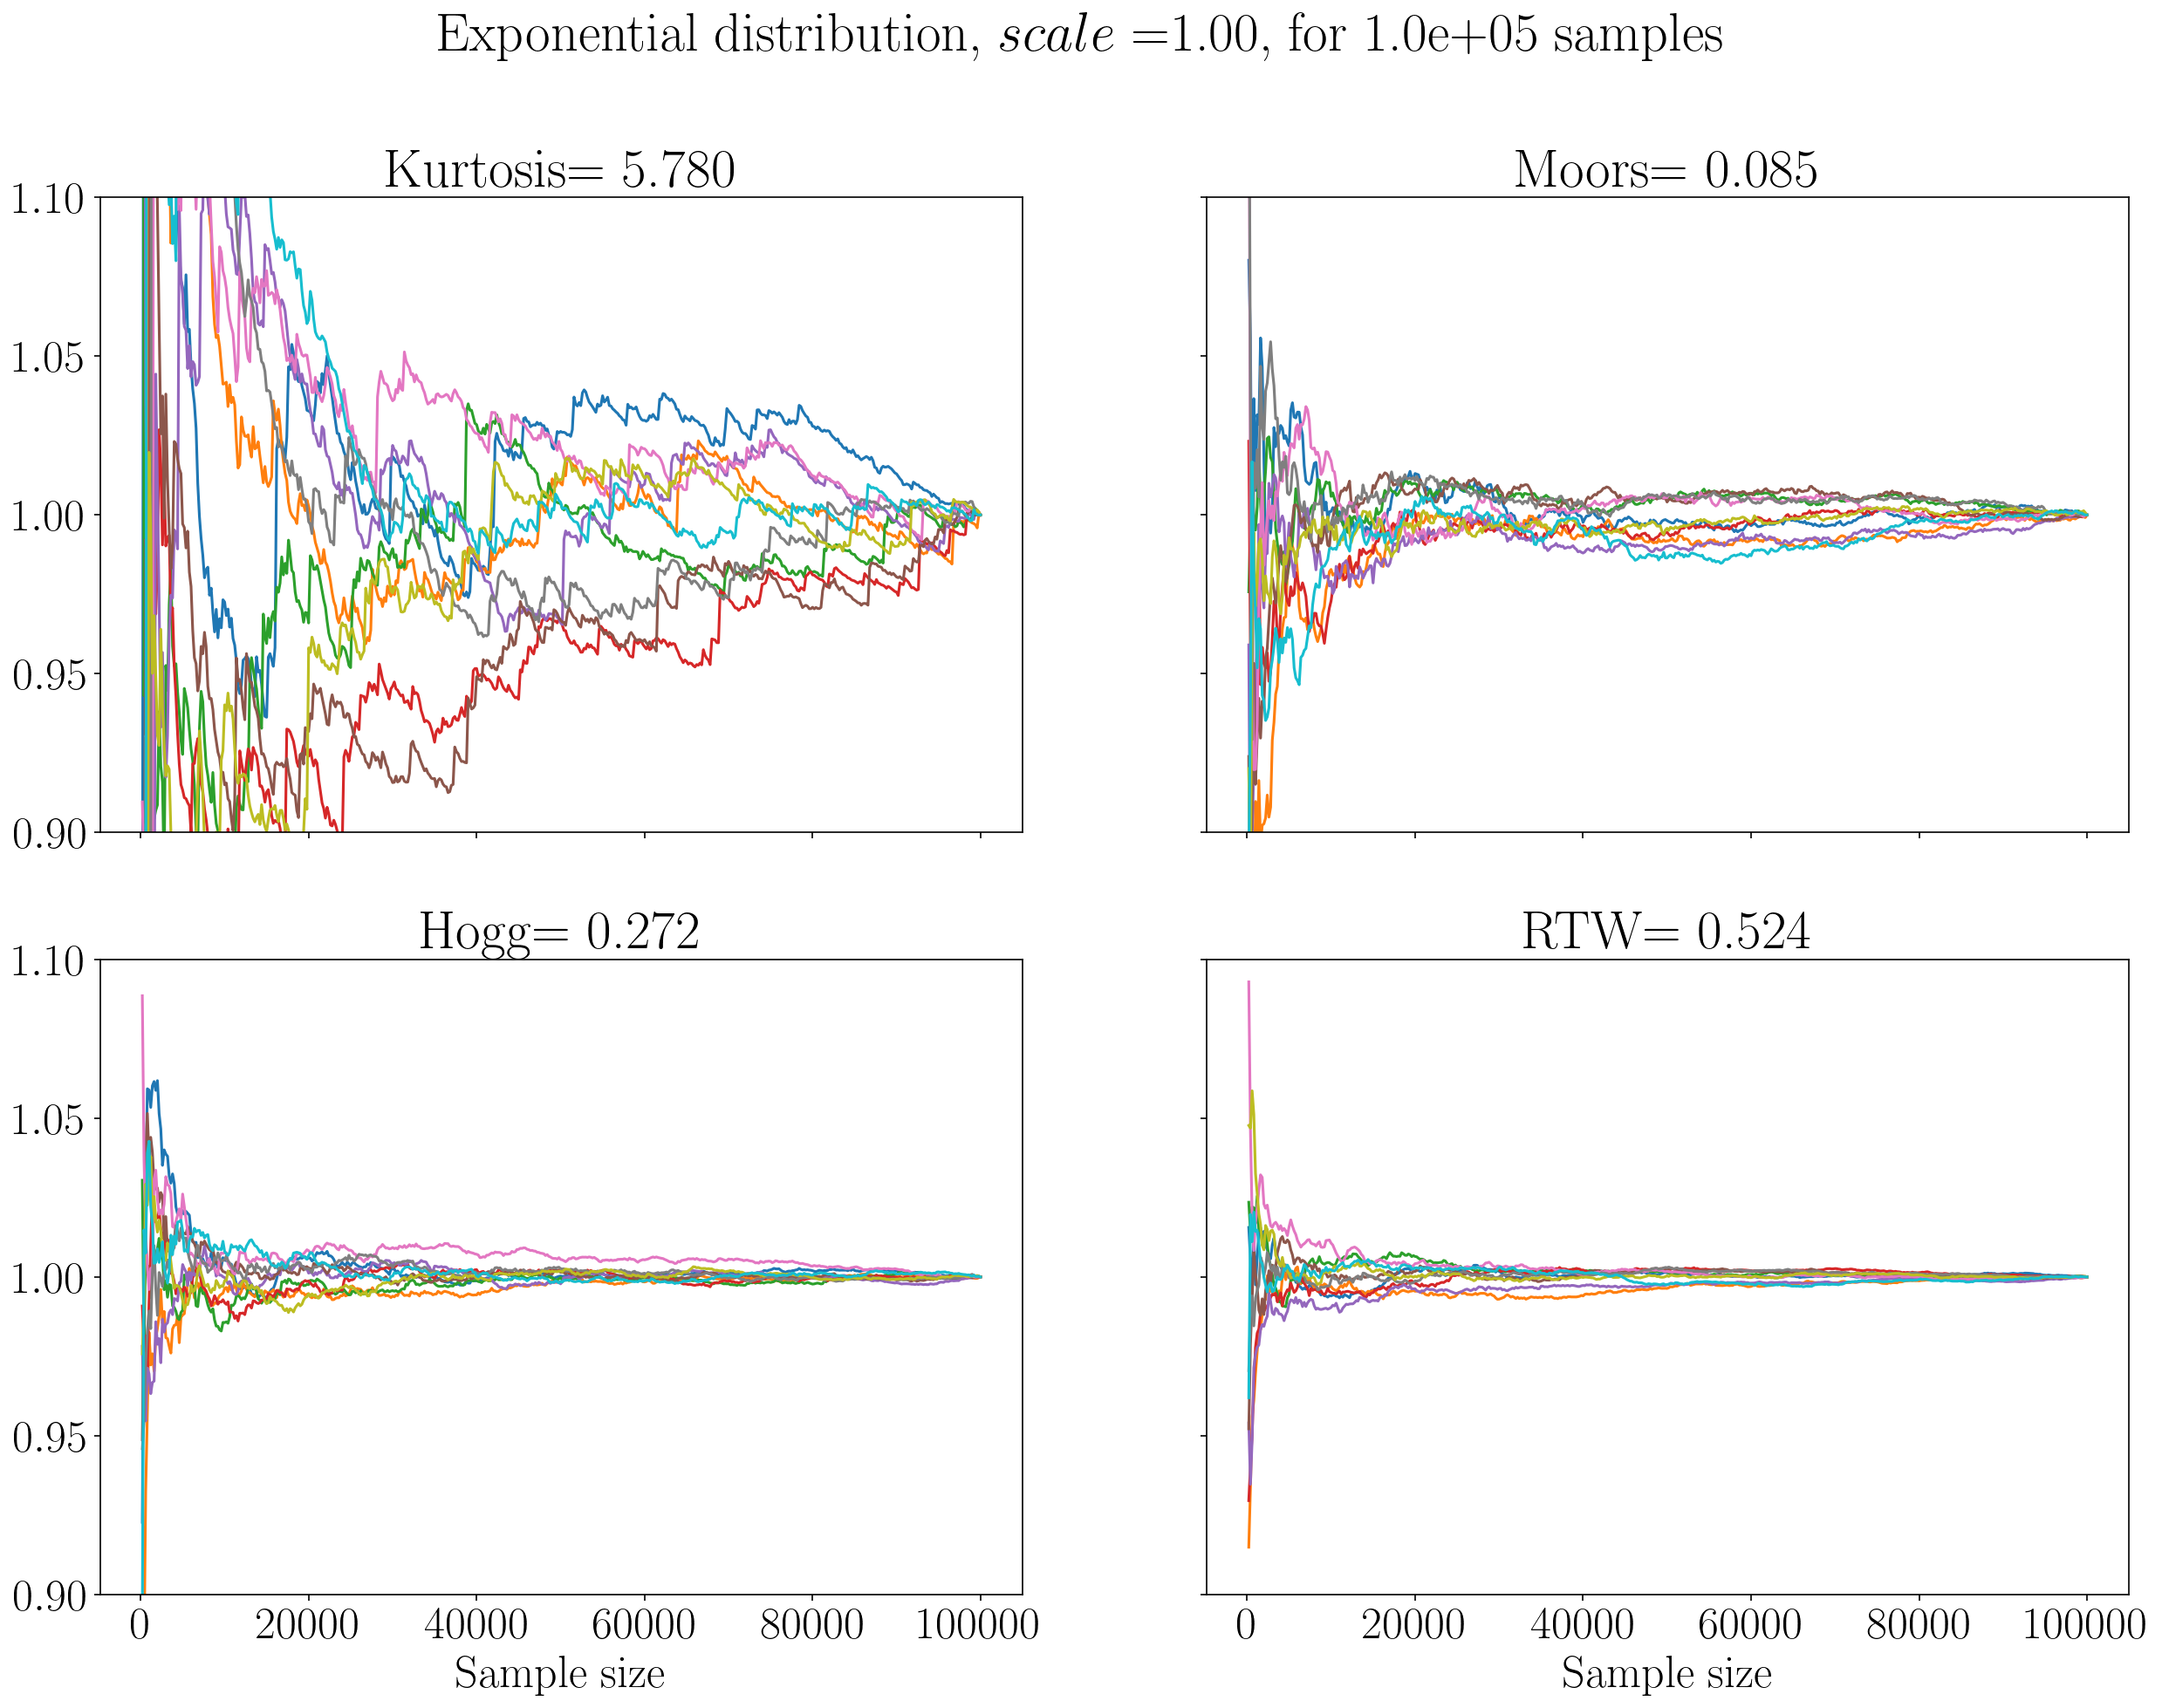
\includegraphics[width=\linewidth]{Images/Metrics/boot_exponential_convergence}
	\caption{ Evolution of the tail statistics: Kurtosis, Moors, Hogg and RTW calculated for an exponential distribution of sample size $10^5$. 
		Each statistic is calculated every $200$ samples. After this is over for all the sample length, the original sample is scrambled and the same procedure is done. This is to show how fast this statistics converge and how much they might fluctuate due to an update of the sample. 
		Each statistic is calculated without correcting for the Gaussian value (ie. is calculated on  the kurtosis, not the excess kurtosis, etc.. ) and normalized to the final value. Only the title values are calculated corrected for the Gaussian values as defined above.}
	\label{fig:bootexponentialconvergence}
\end{figure}

Figure \ref{fig:bootexponentialconvergence} shows the convergence is in statistics doing the same procedure as \cref{fig:convergence_1}, while \cref{fig:boothistogramsexponential} show the same analysis as \cref{fig:Boots_example}.

\begin{figure}[htb]
	\centering
	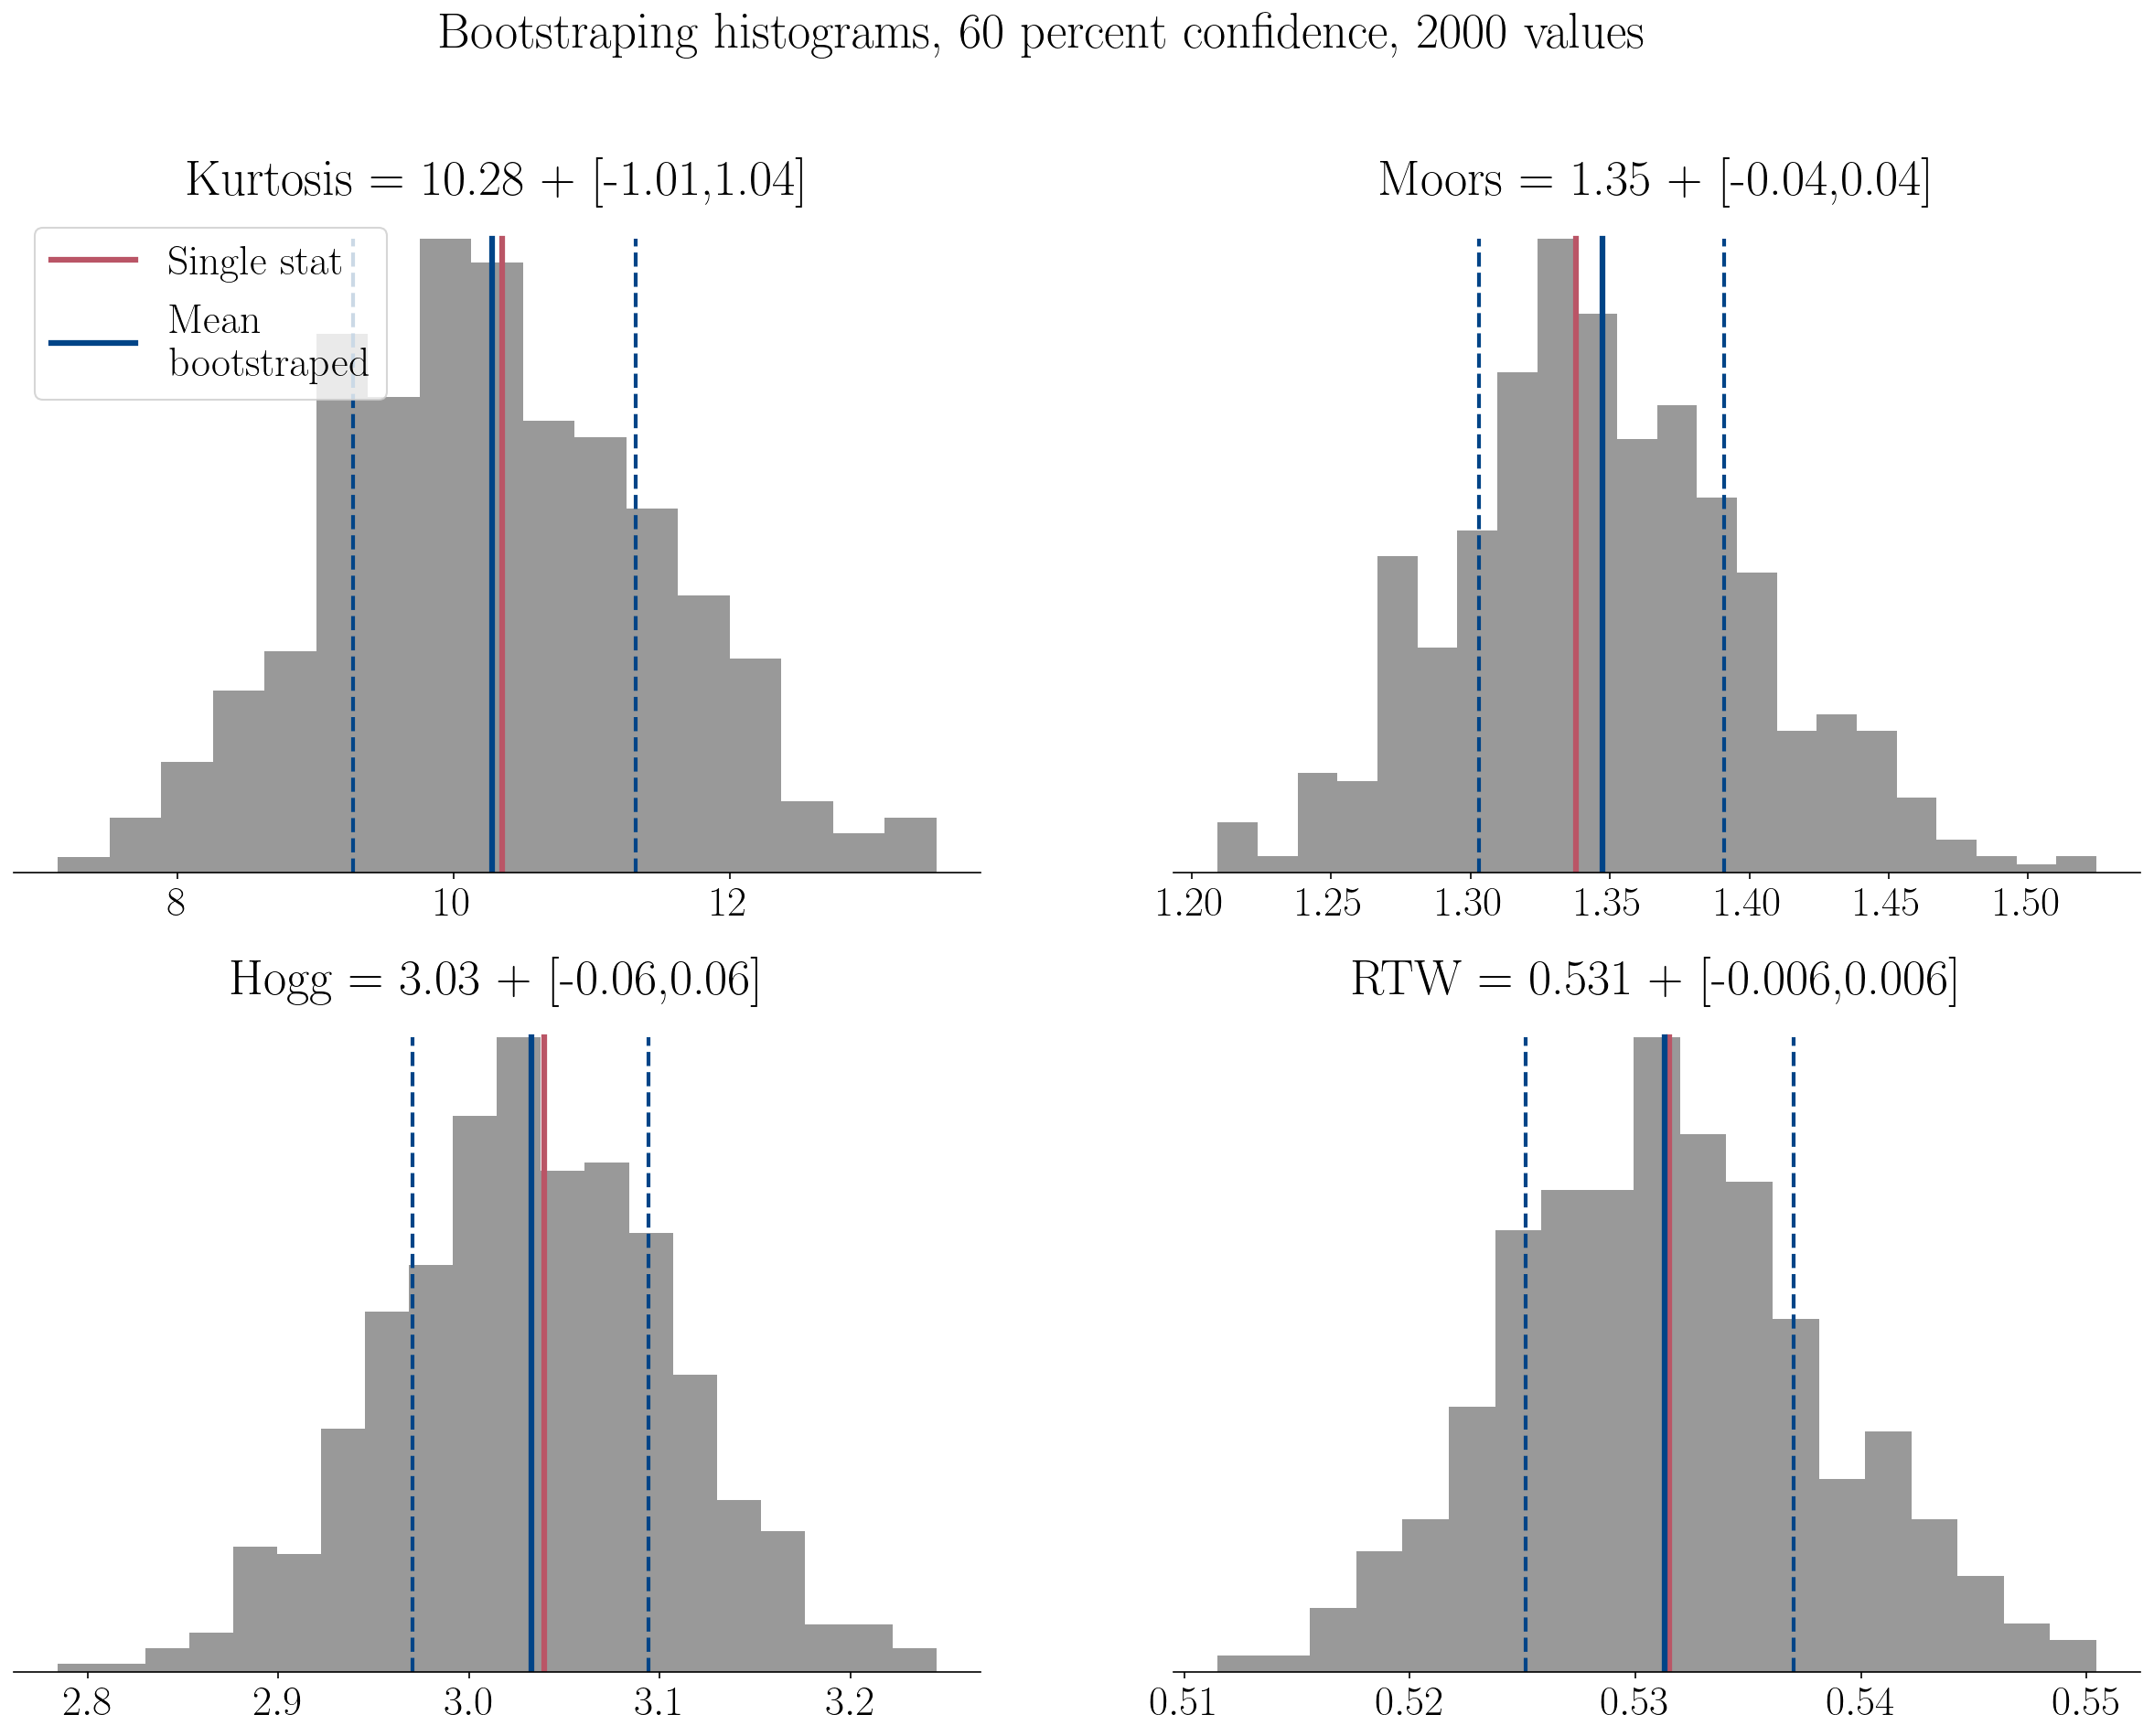
\includegraphics[width=\linewidth]{Images/Metrics/boot_histograms_exponential}
	\caption{ Bootstrapping examples applied to an exponential distribution with 2000 samples, after 600 resamples. The red line indicates the statistic calculated from bootstraping, while the blue line is calculated from the samples, dashed blue indicates the 0.2 and 0.8 percentiles.}
	\label{fig:boothistogramsexponential}
\end{figure}



\section{leftover}

\textbf{Threshold definitions}:
\begin{itemize}
	\item From Ocean Dynamics: $H_f=2H_s $
	\item From Ocean Dynamics (with the definition given above): $H_{m0}=8\sigma$
	\item From Ocean Dynamics: $H_{rms}=2\times 1.4 \text{RMS(H)}$
	\item From Data Minning and descriptive statistics outliers:
	
	$$adj_l=Q_1-1.5r \qquad \qquad adj_H=Q_3+1.5r$$
	
	\item From a talk with Jerome: Another way to define the thresholds could be to make two symmetric distributions based on the original, for each side of the mean. And the take as a threshold some multiple of the standard deviation of this distributions. 
	
	For example, if we want to recover the same value as using $2H_s$ for a Rayleigh distribution, then the new threshold would be the mean of the distribution plus \textbf{$3.69$} times the standard deviation of a symmetrical distribution taken from the right side. 
	
	This way the low intensity threshold can be defined as  the mean od the distribution minus \textbf{$3.69$} times the standard deviation of a symmetrical distribution taken from the lef side, as shown in fig \ref{fig:symthreshrayl} . 
	
	\begin{figure}
		\centering
		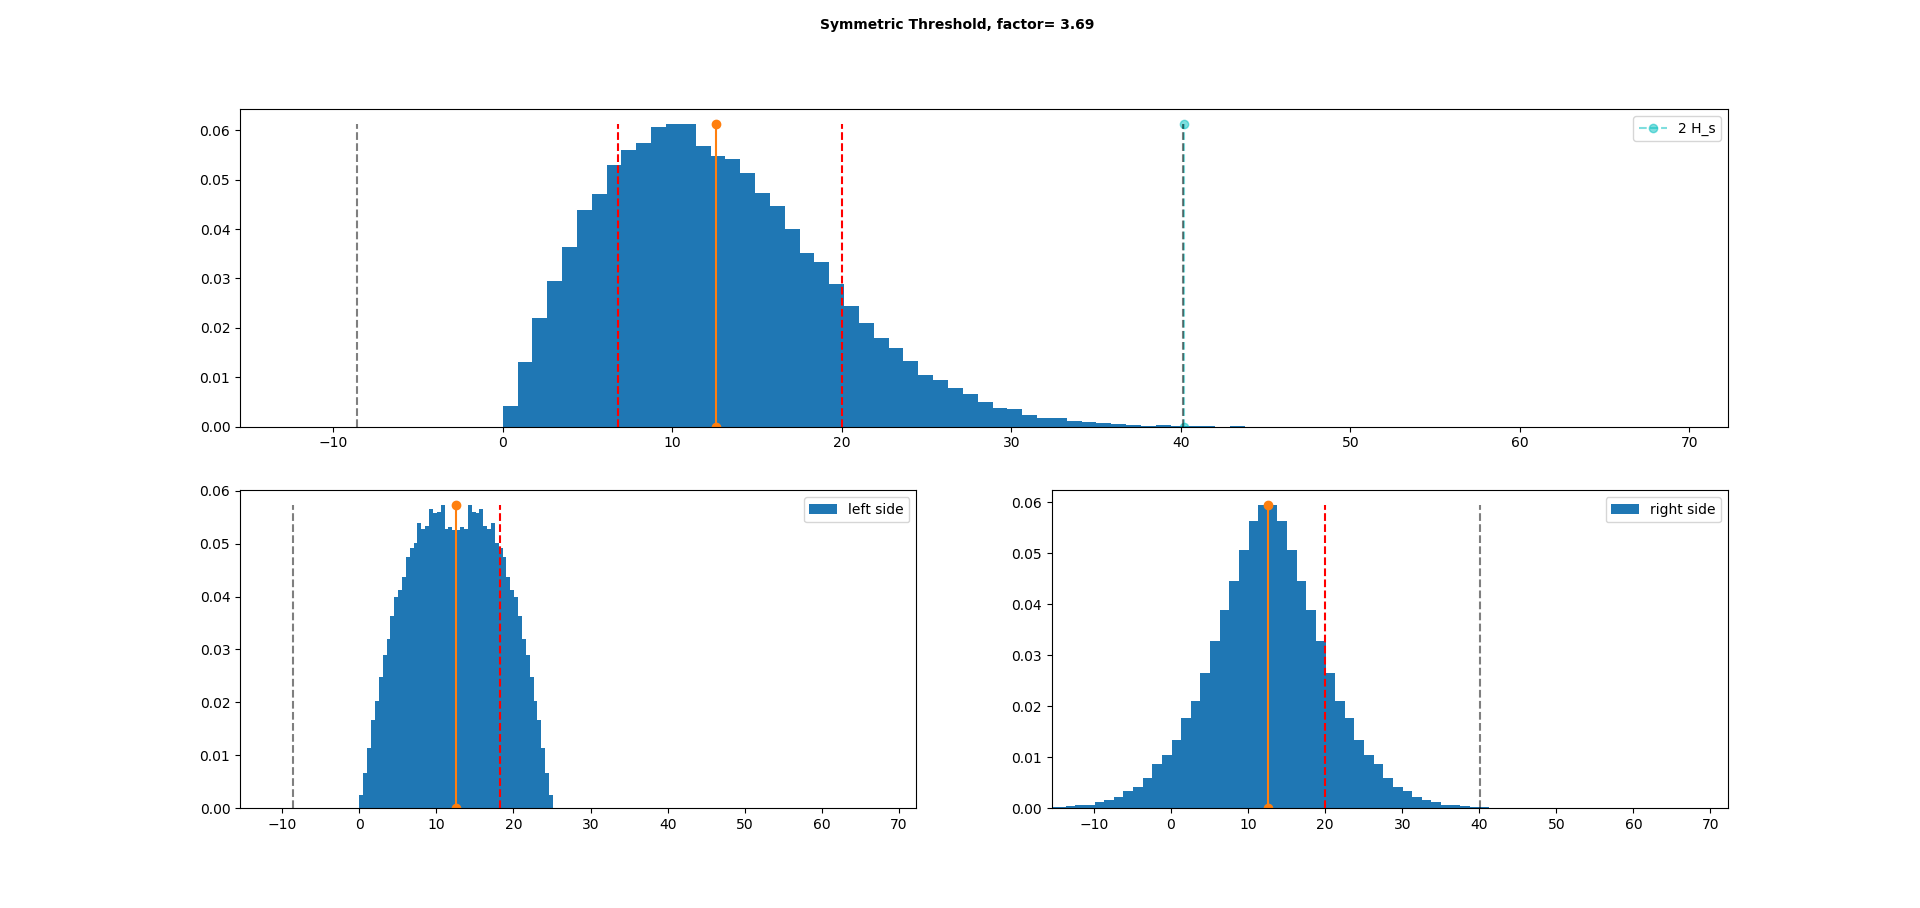
\includegraphics[width=0.8\linewidth]{Images/Metrics/sym_thresh_rayl}
		\caption{Example of the symmetric thresholds for a Rayleigh distribution.}
		\label{fig:symthreshrayl}
	\end{figure}
	
\end{itemize}	

\section{Non equilibrium variance}
\label{apx:variance_contradiction}

At the bifurcation, if the eigenvalues of the Jacobian matrix are real, them $M(x^*,\lambda_c)=0$, this bring forward a possible paradox: \textbf{the equilibrium variance \eqref{eq: ST_variancelim} diverges at $\lambda_c$, but looking at the out of equilibrium factor, it goes to $0$, so the variance might not only not diverge but even vanish at the bifurcation.  }


\begin{equation}
	\lim_{\lambda\to\lambda_c} Var[x]=\frac{\sigma^2}{2 ||M(x^*,\lambda)||}(1-e^{-2M(x^*,\lambda)	\int_{\lambda_0}^{\lambda(t)} \frac{d\lambda}{\dot \lambda}})=\frac{"0"}{"0"}
	\label{eq: ST_lamblim}
\end{equation}

We will see with a simple example that what happens here is that, since we arrive at the bifurcation at a finite time due to the sweeping parameter, the variance of the ensemble is actually finite. 


	\section{Upper constraint of the integration scheme.}
	\label{apx:param_speed_integration}
	
	In the integration scheme there is a limit to how big the time step can be, given a relaxation time $t^*=||M||^{-1}$.
	
	If the time step ($\Delta t$) is larger than the relaxation time ($t^*$) then the system cannot relax to the equilibrium stable ($x^*$) and it becomes unstable.
	
	\begin{figure}
		\centering
		\begin{tikzpicture}
			\node (time) at (11,0)  [right]{$t$};
			\draw [->,very thick,black](0,0) -- (11,0);
			\node[above,left] at (0,3) {a)};
			\foreach \i in {0,...,4}
			{ \draw (2*\i,0) node[rectangle, thin,left color=col2, right color=white!,shading angle=180,anchor=south west, minimum height=3cm,minimum width=2cm,opacity=0.2+\i*(1-0.2)/9] () {}; }
			\foreach \i in {0,...,5}
			{ \filldraw (2*\i,0) circle [circle,black,fill=black,align=center,radius=0.05cm] ; }
			\node[below] (a) at (0,0) [center,below]{$t_i$};
			\node[below] (b) at (2,0) [center,below]{$t_{i+1}$};
			\node[below] (b) at (4,0) [center,below]{$t_{i+2}$};
			\draw [dotted , thick , black,right](6,-0.3) -- (8,-0.3);
			\node[below] (b) at (10,0) [center,below]{$t_{n}$};
			\tzfn[->,col1,ultra thick]{3.5*exp(-1.3*\x)}[0.1:1.5]{}[al]		
		\end{tikzpicture}
		
		\begin{tikzpicture}
			\node (time) at (11,0)  [right]{$t$};
			\draw [->,very thick,black](0,0) -- (11,0);
			\foreach \i in {0,...,9}
			{ \draw (1*\i,0) node[rectangle,  thin,left color=col2, right color=white!,shading angle=180,anchor=south west ,anchor=south west, minimum height=3cm,minimum width=1cm,opacity=0.2+\i*(1-0.2)/9] () {}; }
			\foreach \i in {0,...,10}
			{ \filldraw (1*\i,0) circle [circle,black,fill=black,align=center,radius=0.05cm] ; }
			\node[below] (a) at (0,0) [center,below]{$t_i$};
			\node[below] (b) at (1,0) [center,below]{$t_{i+1}$};
			\node[below] (b) at (2,0) [center,below]{$t_{i+2}$};
			\draw [dotted , thick , black,right](6,-0.3) -- (8,-0.3);
			\node[below] (b) at (10,0) [center,below]{$t_{n}$};		
			\tzfn[->,col1,ultra thick]{3.5*exp(-1.3*\x)}[0.1:1.5]{}[ar]
			\node[above,left] at (0,3) {b)};	
		\end{tikzpicture}
		\caption{a) Small $\Delta t$. b) Big $\Delta t$. For a given value of $t^*=||M(\lambda)||^{-1}$ the system has a well defined relaxation timescale. Ideally the times array should change slow enough for the system to be able to 'relax'.}
		\label{fig: velocity_param2}
	\end{figure}
	
	
	Therefore we choose $ \Delta t < min(t^*)/2 $ where $min(t^*)$ is the smallest relaxation time over the evolution of the parameter $\lambda$.
	Thus the $\Delta t$ is determined by the region with highest \textit{resilience}, far from the b-tipping bifurcation. 
	
	$t_{var}=\frac{1}{2M}=min(t^*)/2$
	
	
	$ \Delta t < min(t^*)/4 $
	


Warning of a forthcoming collapse of the Atlantic
meridional overturning circulation

On Conditions for Rate-induced Tipping in Multi-dimensionalDynamical Systems


\subsection{Sharp transition mockup}	
\label{ewsapx: transition}
%\ag{Describe the data: simulated data for each numerical experiment; Goery's data, filament data [with Experimental setup if we want to include them.]}

Since we want to have a data set where we can control the 'tailedness' of the distribution, we will use a couple toy models thought specifically to have a smooth transition between random data with a normal distribution, to a distribution with an arbitrary large tail. 

We also show the same method applied to a real data set with a phase transition.

\subsubsection{Simulation of an experimental transition.}
The goal of this test is to understand how a signal for a quick transition might look on the tail related statistics. To do this we test adding noise to an Error function.

%simulate what one might see if acquiring data while going through a sharp or smooth transition between two given values.
The noise is added by a background Gaussian noise in the data, and a Gaussian indetermination of the experimental parameter (sampling Gaussian) at which the measurement takes place \footnote{For example: Measuring a transition in conductivity for different temperatures. 
	In this case we suppose there would be a Gaussian fluctuation for the temperature at which we set the experiment, and there is some background noise in the instrument we use to measure the conductivity. }. 
In this case the 'sharpness' transition is controlled by the transition window (the slope of the Erf function) compared to the noise from the sampling Gaussian $\sigma$.

Each data point is generated by 
\begin{equation}
	\mathrm{Erf}(z)=\frac{2}{\sqrt{\pi}}\int_0^z e^{-t^2}
\end{equation}

\begin{equation}
	y_j=A_0\left(\mathrm{ Erf} \left( \frac{(x_j)}{\sqrt{2}s_2}\right)+1\right)+y_0+n_0
\end{equation}

Where $n_0$ is a random value taken from a normal distribution N(0,$\sigma_{n_0}$), $y_0$ is an offset for the lower value of the Erf function. 
$x_j$ is a random number generated by a normal distribution $N(\mu,\sigma)$, and $S_2$ is  a parameter that controls the slope (and the width of the transition) as shown in figure \ref{fig:transition_example}. 

\begin{figure}[htb]
	\centering
	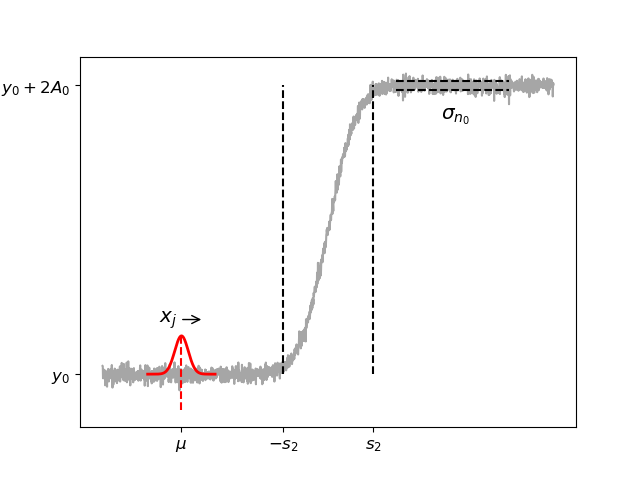
\includegraphics[width=0.7\linewidth]{Images/Metrics/erf_example.png}
	\caption{ Sketch for smooth transition between the mean values $y_0$ and $y_0+2A_0$ using an $\mathrm{Erf}$ function. The dispersion around such values is given by $\sigma_{n_0}$, and the transition occurs between $-s_2$ and $s_2$.
		In red it is shown the sampling Gaussian that simulates an imperfect measurement device or indetermination of an experimental parameter. 
		This example has $\sigma_{n_0}=0.06$, $\sigma=0.6$, $A0=2$ and  $S_2=1$.}
	\label{fig:transition_example}
\end{figure}
Changing the value of $\mu$ is equivalent to acquiring data from a given point in the Erf function, where there is inherent  noise both in the data acquired and the value of $\mu$ for which one acquires the data. 

Therefore acquiring data far from the transition gives a Gaussian result with a variance of $\sigma_{n_0}$, and changes as $\mu$ approaches the transition. 

This gives two parameters to characterize a transition between two values.
$\frac{\sigma_{n_0}}{A_0}$ reflects the relation between the noise and the distance between the steady values $y_0$ and $y_0+A_0$. 
$\frac{\sigma_{n_0}}{A_0}<1$ gives a big transition, while $\frac{\sigma_{n_0}}{A_0}>1$ gives a small transition. $\frac{\sigma}{s_2}$ reflects the relation between the noise of the sampling Gaussian transition length; $\frac{\sigma}{s_2}<1$ gives a smooth transition, while $\frac{\sigma}{s_2}>1$ gives a sharp transition. Such different possible dynamics can be seen in figure \ref{fig:transition_configurations}.
\footnote{\ag{i'm not sure it should be $s_2$ or $2s_2$; and $A0$ or $2A0$.Rta: I think it should be $\sigma/s_2$ and $2\sigma_{n_0}/A_0$ since this gives overlap in the highest $10 \%$  of the gaussians, I need to change the text and simulations at some point to show this. }}.


%\begin{figure}[h]
%\centering
%    	\includegraphics[width=0.45\linewidth]{images/metric/simulation-transition/erf_example_transition_stats.png}
%   	\includegraphics[width=0.45\linewidth]{images/metric/simulation-transition/erf_example_transition_stats2.png}\\
%  	\includegraphics[width=0.45\linewidth]{images/metric/simulation-transition/erf_example_transition_stats3.png}
% 	\includegraphics[width=0.45\linewidth]{images/metric/simulation-transition/erf_example_transition_stats4.png}
%\caption{ Two possible behaviours for the transition statistics, depending on the relation between $s_2$ and $\sigma$. a)$\frac{\sigma_{n_0}}{A_0}$= 0.03 $\frac{\sigma}{s_2}$=2, b)$\frac{\sigma_{n_0}}{A_0}$= 0.03 $\frac{\sigma}{s_2}$=0.6 , c)$\frac{\sigma_{n_0}}{A_0}$= 1.25 $\frac{\sigma}{s_2}$=2,
	%   	d)$\frac{\sigma_{n_0}}{A_0}$= 1.25 $\frac{\sigma}{s_2}$=0.6 . Each histogram is plotted in log scale using a the 'blocks' method from the  %\texttt{astropy.stats.histogram} dependency to be able to better show the long tales. \ag{change the fraction display}}
%\label{fig:transition_configurations}
%first case:  \sigma_n0=0.06, sigma=2, A0=2, S2=1
%second case: \sigma_n0=0.06, sigma=0.6, A0=2, S2=1
%third case:\sigma_n0=2.5, sigma=2, A0=2, S2=1
%forth case:\sigma_n0=2.5, sigma=0.6, A0=2, S2=1
%\end{figure}

\begin{figure}[H]
	\centering
	\includegraphics[width=0.45\linewidth]{Images/Metrics/erf_example_transition_stats_3da.png}
	\includegraphics[width=0.45\linewidth]{Images/Metrics/erf_example_transition_stats_3db.png}\\
	\includegraphics[width=0.45\linewidth]{Images/Metrics/erf_example_transition_stats_3dc.png}
	\includegraphics[width=0.45\linewidth]{Images/Metrics/erf_example_transition_stats_3dd.png}
	\caption{ \sout{Two} possible behaviours for the transition statistics, depending on the relation between $s_2$ and $\sigma$. a)$\frac{\sigma_{n_0}}{A_0}$= 0.03 $\frac{\sigma}{s_2}$=2, b)$\frac{\sigma_{n_0}}{A_0}$= 0.03 $\frac{\sigma}{s_2}$=0.4 , c)$\frac{\sigma_{n_0}}{A_0}$= 1.25 $\frac{\sigma}{s_2}$=2,
		d)$\frac{\sigma_{n_0}}{A_0}$= 1.25 $\frac{\sigma}{s_2}$=0.4 . Each histogram is plotted in log scale using the 'blocks' method from the  \texttt{astropy.stats.histogram} dependency to be able to better show the long tales. \ag{change the fraction display} \mb{Use larger font in labels!}}
	\label{fig:transition_configurations}
	%first case:  \sigma_n0=0.06, sigma=2, A0=2, S2=1
	%second case: \sigma_n0=0.06, sigma=0.5, A0=2, S2=1
	%third case:\sigma_n0=2.5, sigma=2, A0=2, S2=1
	%forth case:\sigma_n0=2.5, sigma=0.4, A0=2, S2=1
\end{figure}
For $\mu=0$ (the symmetric case), when  $\frac{\sigma}{s_2}=1$ the resulting distribution is close to a uniform distribution when $\frac{\sigma_{n_0}}{A_0}<1$. This means that the transition between low and high values of $\frac{\sigma}{s_2}$, for $\mu=0$  and low $\frac{\sigma_{n_0}}{A_0}$ is a continuous transition between a Gaussian to a bi-modal distribution, going though a normal distribution.  

Other possibilities to explore for transitions is the extreme case of a heavyside function, or the case where the transition happens in the slope of a linear signal. 


\section{Overshoot tipping with high noise}

A particular case that has not been explore sufficiently in the literature is the case of a moving parameter that returns to it's initial value, goes though a bifurcation of the autonomous system along it's evolution, but also presents some 'high' stochastic noise. 



Here we consider the system 

\begin{equation}
	\begin{cases}
		dx&=(-x^3+0.9x+\lambda)dt+\sigma dW\\
		d\lambda&=2(-(\la_0+\la_{max})/(t_f/2)^2)(t-t_f/2)\\
		\lambda(t_0=0)&=\lambda(t=t_f)=\lambda_0
	\end{cases}
\end{equation} 

Here the speed of the parameter is defined by the final time $t_f$.

With very low noise, the system behaves as in \cref{fig:overshoot2}, however, if we set $\sigma=0.1$ we can see different behaviours due to the stochasticity of the system. 

Figures \ref{fig:overshootnoise4,fig:overshootnoise2,fig:overshootnoise3} show three independent realizations of this system, with the same parameters, where in \textcolor{col1}{yellow} we show a slow sweeping, in \textcolor{col2}{red} an intermediate sweeping and in \textcolor{col3}{blue} a fast sweeping (just like in \cref{fig:overshoot2}). 
However in this case, the intermediate and fast sweeped integration might or might not tip to the lower stable branch depending on the stochastic path the system might take.

\begin{figure}
	\centering
	\includegraphics[width=0.9\linewidth]{Images/Metrics/overshoot_noise4}
	\caption{}
	\label{fig:overshootnoise4}
\end{figure}

\begin{figure}
	\centering
	\includegraphics[width=0.9\linewidth]{Images/Metrics/overshoot_noise2}
	\caption{}
	\label{fig:overshootnoise2}
\end{figure}

\begin{figure}
	\centering
	\includegraphics[width=0.9\linewidth]{Images/Metrics/overshoot_noise3}
	\caption{}
	\label{fig:overshootnoise3}
\end{figure}

\Cref{fig:overshootnoise4} shows a case where neither the fast and intermediate sweeped parameters tip, while \cref{fig:overshootnoise2} show both cases tipping, and \ref{fig:overshootnoise3} shows the intermediate sweeped parameter tipping while the fast parameter does not, as in the deterministic systems.  

This examples highlight the important of studying the ASS system as compared to the deterministic augmented system or to a stochastic systems where the control parameter does not change continuously. 
In this example the  tipping mechanism (B,R,N-tipping) are relevant at the same time. 

\section{triangle}

\begin{figure}[htb]
	\centering
	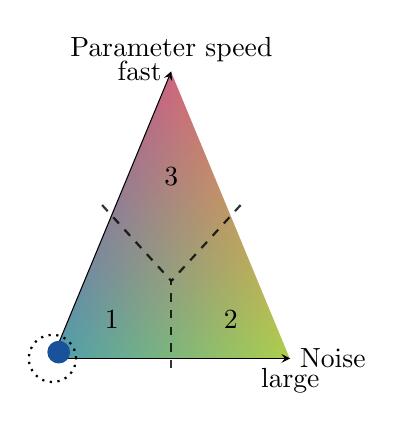
\begin{tikzpicture}
		\draw (0,0) node[isosceles triangle, thin,left color=blue!90, right color=orange!90,shading angle=90,anchor=left corner, minimum size =3cm,rotate=90,opacity=0.7] (T1) at (0,0){};
		\draw (0,0) node[isosceles triangle, thin,left color=green!80, right color=red!80,shading angle=180,anchor=left corner, minimum size =3cm,rotate=90,opacity=0.4] (T1) at (0,0){};
		\draw [->,opacity=1](0,0) node[below] {} -- (T1.right corner)  node[right] {Noise} node[below] {large};
		\draw [->,opacity=1](0,0) node[left] {} -- (T1.apex) node[above] {Parameter speed} node[left] {fast} ;
		\node (a) at (0.08,0.08) {};
		\node (b) at (T1.right side) {};
		\node (c) at (T1.left side) {};
		\node (d) at (T1.west) {};
		\draw [dashed,opacity=0.8,thick] (b.north east) -- (T1.center) node {} ;
		
		\draw [dashed,opacity=0.8,thick] (c.north west) -- 	(T1.center) node {} ;
		
		\draw [dashed,opacity=0.8,thick] (d.south) -- 	(T1.center) node {} ;
		
		\draw [dotted,thick] (0,0) circle [radius=0.3cm,draw=black] ;
		
		\node (e) at ($(T1.apex)!0.5!(T1.center)$) {$3$};
		\node (f) at ($(0,0)!0.5!(T1.center)$) {$1$};
		\node (g) at ($(T1.right corner)!0.5!(T1.center)$) {$2$};
		
		
		\filldraw [blue!70!green!80!black!90,thick] (a.center) circle [radius=0.13cm,draw=black];
	\end{tikzpicture}
	\caption{We focus on slow change of parameters and small additive noise.}        
	\label{fig: noise_transition2}
\end{figure}


	\end{appendices}
	\pagebreak
	
	\bibliographystyle{plainnat}
	%\bibliographystyle{unsrt}
	\bibliography{Bibliography/Thesis_bib}
	
\end{document}